
%% 
%% Copyright 2007, 2008, 2009 Elsevier Ltd
%% 
%% This file is part of the 'Elsarticle Bundle'.
%% ---------------------------------------------
%% 
%% It may be distributed under the conditions of the LaTeX Project Public
%% License, either version 1.2 of this license or (at your option) any
%% later version.  The latest version of this license is in
%%    http://www.latex-project.org/lppl.txt
%% and version 1.2 or later is part of all distributions of LaTeX
%% version 1999/12/01 or later.
%% 
%% The list of all files belonging to the 'Elsarticle Bundle' is
%% given in the file `manifest.txt'.
%% 
%% Template article for Elsevier's document class `elsarticle'
%% with harvard style bibliographic references
%% SP 2008/03/01

\documentclass[preprint,12pt,authoryear]{elsarticle}

%% Use the option review to obtain double line spacing
%% \documentclass[authoryear,preprint,review,12pt]{elsarticle}

%% Use the options 1p,twocolumn; 3p; 3p,twocolumn; 5p; or 5p,twocolumn
%% for a journal layout:
%% \documentclass[final,1p,times,authoryear]{elsarticle}
%% \documentclass[final,1p,times,twocolumn,authoryear]{elsarticle}
%% \documentclass[final,3p,times,authoryear]{elsarticle}
%% \documentclass[final,3p,times,twocolumn,authoryear]{elsarticle}
%% \documentclass[final,5p,times,authoryear]{elsarticle}
%% \documentclass[final,5p,times,twocolumn,authoryear]{elsarticle}

\usepackage[T1]{fontenc}
\usepackage[utf8]{inputenc}

\usepackage{algorithm}
\usepackage{algorithmic}

%% For including figures, graphicx.sty has been loaded in
%% elsarticle.cls. If you prefer to use the old commands
%% please give \usepackage{epsfig}
%\usepackage{graphicx}

%% The amssymb package provides various useful mathematical symbols
\usepackage{amssymb}
\usepackage{amsmath}
%% The amsthm package provides extended theorem environments
\usepackage{amsthm}
\newtheorem{theorem}{Theorem}

\usepackage{color}

\usepackage{subfig}

%% The lineno packages adds line numbers. Start line numbering with
%% \begin{linenumbers}, end it with \end{linenumbers}. Or switch it on
%% for the whole article with \linenumbers.
%% \usepackage{lineno}

\journal{Neucocomputing}

%%% Adding metadata:
\newsubfloat{figure}
\newsubfloat{table}
% Better page layout for A4 paper, see memoir manual.
\settrimmedsize{297mm}{210mm}{*}
\setlength{\trimtop}{0pt} 
\setlength{\trimedge}{\stockwidth} 
\addtolength{\trimedge}{-\paperwidth} 
\settypeblocksize{634pt}{448.13pt}{*} 
\setulmargins{4cm}{*}{*} 
\setlrmargins{*}{*}{1.5} 
\setmarginnotes{17pt}{51pt}{\onelineskip} 
\setheadfoot{\onelineskip}{2\onelineskip} 
\setheaderspaces{*}{2\onelineskip}{*} 
\checkandfixthelayout
%
\frenchspacing
% Font with math support: New Century Schoolbook
\usepackage{fouriernc}
\usepackage[T1]{fontenc}
%
% UoB guidelines:
%
% Text should be in double or 1.5 line spacing, and font size should be
% chosen to ensure clarity and legibility for the main text and for any
% quotations and footnotes. Margins should allow for eventual hard binding.
%
% Note: This is automatically set by memoir class. Nevertheless \OnehalfSpacing 
% enables double spacing but leaves single spaced for captions for instance. 
\OnehalfSpacing 
%
% Sets numbering division level
\setsecnumdepth{subsection} 
\maxsecnumdepth{subsubsection}
%
% Chapter style (taken and slightly modified from Lars Madsen Memoir Chapter 
% Styles document
\usepackage{calc,soul,fourier}

\iffalse
\makeatletter 
\newlength\dlf@normtxtw 
\setlength\dlf@normtxtw{\textwidth} 
\newsavebox{\feline@chapter} 
\newcommand\feline@chapter@marker[1][4cm]{%
	\sbox\feline@chapter{% 
		\resizebox{!}{#1}{\fboxsep=1pt%
			\colorbox{gray}{\color{white}\thechapter}% 
		}}%
		\rotatebox{90}{% 
			\resizebox{%
				\heightof{\usebox{\feline@chapter}}+\depthof{\usebox{\feline@chapter}}}% 
			{!}{\scshape\so\@chapapp}}\quad%
		\raisebox{\depthof{\usebox{\feline@chapter}}}{\usebox{\feline@chapter}}%
} 
\newcommand\feline@chm[1][4cm]{%
	\sbox\feline@chapter{\feline@chapter@marker[#1]}% 
	\makebox[0pt][c]{% aka \rlap
		\makebox[1cm][r]{\usebox\feline@chapter}%
	}}
\makechapterstyle{daleifmodif}{
	\renewcommand\chapnamefont{\normalfont\Large\scshape\raggedleft\so} 
	\renewcommand\chaptitlefont{\normalfont\Large\bfseries\scshape} 
	\renewcommand\chapternamenum{} \renewcommand\printchaptername{} 
	\renewcommand\printchapternum{\null\hfill\feline@chm[2.5cm]\par} 
	\renewcommand\afterchapternum{\par\vskip\midchapskip} 
	\renewcommand\printchaptertitle[1]{\color{gray}\chaptitlefont\raggedleft ##1\par}
} 
\makeatother 
\chapterstyle{daleifmodif}
\fi
%
% UoB guidelines:
%
% The pages should be numbered consecutively at the bottom centre of the
% page.
\makepagestyle{myvf} 
\makeoddfoot{myvf}{}{\thepage}{} 
\makeevenfoot{myvf}{}{\thepage}{} 
\makeheadrule{myvf}{\textwidth}{\normalrulethickness} 
\makeevenhead{myvf}{\small\textsc{\leftmark}}{}{} 
\makeoddhead{myvf}{}{}{\small\textsc{\rightmark}}
\pagestyle{myvf}
%
% Oscar's command (it works):
% Fills blank pages until next odd-numbered page. Used to emulate single-sided
% frontmatter. This will work for title, abstract and declaration. Though the
% contents sections will each start on an odd-numbered page they will
% spill over onto the even-numbered pages if extending beyond one page
% (hopefully, this is ok).
\newcommand{\clearemptydoublepage}{\newpage{\thispagestyle{empty}\cleardoublepage}}
%
%
% Creates indexes for Table of Contents, List of Figures, List of Tables and Index
\makeindex
% \printglossaries below creates a list of abbreviations. \gls and related
% commands are then used throughout the text, so that latex can automatically
% keep track of which abbreviations have already been defined in the text.
%
% The import command enables each chapter tex file to use relative paths when
% accessing supplementary files. For example, to include
% chapters/brewing/images/figure1.png from chapters/brewing/brewing.tex we can
% use
% \includegraphics{images/figure1}
% instead of
% \includegraphics{chapters/brewing/images/figure1}
\usepackage{import}

% Add other packages needed for chapters here. For example:
\usepackage{lipsum}					%Needed to create dummy text
\usepackage{amsfonts} 					%Calls Amer. Math. Soc. (AMS) fonts
\usepackage[centertags]{amsmath}			%Writes maths centred down
\usepackage{stmaryrd}					%New AMS symbols
\usepackage{amssymb}					%Calls AMS symbols
\usepackage{amsthm}					%Calls AMS theorem environment
\usepackage{newlfont}					%Helpful package for fonts and symbols
\usepackage{layouts}					%Layout diagrams
\usepackage{graphicx}					%Calls figure environment
\usepackage{longtable,rotating}			%Long tab environments including rotation. 
\usepackage[utf8]{inputenc}			%Needed to encode non-english characters 
									%directly for mac
\usepackage{colortbl}					%Makes coloured tables
\usepackage{wasysym}					%More math symbols
\usepackage{mathrsfs}					%Even more math symbols
\usepackage{float}						%Helps to place figures, tables, etc. 
\usepackage{verbatim}					%Permits pre-formated text insertion
\usepackage{upgreek }					%Calls other kind of greek alphabet
\usepackage{latexsym}					%Extra symbols
\usepackage[square,numbers,
		     sort&compress]{natbib}		%Calls bibliography commands 
\usepackage{url}						%Supports url commands
\usepackage{etex}						%eTeXÕs extended support for counters
\usepackage{fixltx2e}					%Eliminates some in felicities of the 
									%original LaTeX kernel
\usepackage[spanish,english]{babel}		%For languages characters and hyphenation
\usepackage{color}                    				%Creates coloured text and background
\usepackage[colorlinks=true,
		     allcolors=black]{hyperref}              %Creates hyperlinks in cross references
\usepackage{memhfixc}					%Must be used on memoir document 
									%class after hyperref
\usepackage{enumerate}					%For enumeration counter
\usepackage{footnote}					%For footnotes
\usepackage{microtype}					%Makes pdf look better.
\usepackage{rotfloat}					%For rotating and float environments as tables, 
									%figures, etc. 
\usepackage{alltt}						%LaTeX commands are not disabled in 
									%verbatim-like environment
\usepackage[version=0.96]{pgf}			%PGF/TikZ is a tandem of languages for producing vector graphics from a 
\usepackage{tikz}						%geometric/algebraic description.
\usetikzlibrary{arrows,shapes,snakes,
		       automata,backgrounds,
		       petri,topaths}				%To use diverse features from tikz		
%							
%Reduce widows  (the last line of a paragraph at the start of a page) and orphans 
% (the first line of paragraph at the end of a page)
\widowpenalty=1000
\clubpenalty=1000
%
% New command definitions for my thesis
%

\newcommand{\keywords}[1]{\par\noindent{\small{\bf Keywords:} #1}} %Defines keywords small section
\newcommand{\parcial}[2]{\frac{\partial#1}{\partial#2}}                             %Defines a partial operator
\newcommand{\vectorr}[1]{\mathbf{#1}}                                                        %Defines a bold vector
\newcommand{\vecol}[2]{\left(                                                                         %Defines a column vector
	\begin{array}{c} 
		\displaystyle#1 \\
		\displaystyle#2
	\end{array}\right)}
\newcommand{\mados}[4]{\left(                                                                       %Defines a 2x2 matrix
	\begin{array}{cc}
		\displaystyle#1 &\displaystyle #2 \\
		\displaystyle#3 & \displaystyle#4
	\end{array}\right)}
\newcommand{\pgftextcircled}[1]{                                                                    %Defines encircled text
    \setbox0=\hbox{#1}%
    \dimen0\wd0%
    \divide\dimen0 by 2%
    \begin{tikzpicture}[baseline=(a.base)]%
        \useasboundingbox (-\the\dimen0,0pt) rectangle (\the\dimen0,1pt);
        \node[circle,draw,outer sep=0pt,inner sep=0.1ex] (a) {#1};
    \end{tikzpicture}
}
\newcommand{\range}[1]{\textnormal{range }#1}                                             %Defines range operator
\newcommand{\innerp}[2]{\left\langle#1,#2\right\rangle}                                 %Defines inner product
\newcommand{\prom}[1]{\left\langle#1\right\rangle}                                         %Defines average operator
\newcommand{\tra}[1]{\textnormal{tra} \: #1}                                                       %Defines trace operator
\newcommand{\sign}[1]{\textnormal{sign\,}#1}                                                   %Defines sign operator
\newcommand{\sech}[1]{\textnormal{sech} #1}                                                  %Defines sech
\newcommand{\diag}[1]{\textnormal{diag} #1}                                                    %Defines diag operator
\newcommand{\arcsech}[1]{\textnormal{arcsech} #1}                                       %Defines arcsech
\newcommand{\arctanh}[1]{\textnormal{arctanh} #1}                                         %Defines arctanh
%Change tombstone symbol
\newcommand{\blackged}{\hfill$\blacksquare$}
\newcommand{\whiteged}{\hfill$\square$}
\newcounter{proofcount}
\renewenvironment{proof}[1][\proofname.]{\par
 \ifnum \theproofcount>0 \pushQED{\whiteged} \else \pushQED{\blackged} \fi%
 \refstepcounter{proofcount}
 \normalfont 
 \trivlist
 \item[\hskip\labelsep
       \itshape
   {\bf\em #1}]\ignorespaces
}{%
 \addtocounter{proofcount}{-1}
 \popQED\endtrivlist
}
%
%
% New definition of square root:
% it renames \sqrt as \oldsqrt
\let\oldsqrt\sqrt
% it defines the new \sqrt in terms of the old one
\def\sqrt{\mathpalette\DHLhksqrt}
\def\DHLhksqrt#1#2{%
\setbox0=\hbox{$#1\oldsqrt{#2\,}$}\dimen0=\ht0
\advance\dimen0-0.2\ht0
\setbox2=\hbox{\vrule height\ht0 depth -\dimen0}%
{\box0\lower0.4pt\box2}}
%
% My caption style
\newcommand{\mycaption}[2][\@empty]{
	\captionnamefont{\scshape} 
	\changecaptionwidth
	\captionwidth{0.9\linewidth}
	\captiondelim{.\:} 
	\indentcaption{0.75cm}
	\captionstyle[\centering]{}
	\setlength{\belowcaptionskip}{10pt}
	\ifx \@empty#1 \caption{#2}\else \caption[#1]{#2}
}
%
% My subcaption style
\newcommand{\mysubcaption}[2][\@empty]{
	\subcaptionsize{\small}
	\hangsubcaption
	\subcaptionlabelfont{\rmfamily}
	\sidecapstyle{\raggedright}
	\setlength{\belowcaptionskip}{10pt}
	\ifx \@empty#1 \subcaption{#2}\else \subcaption[#1]{#2}
}
%
%An initial of the very first character of the content
\usepackage{lettrine}
\newcommand{\initial}[1]{%
	\lettrine[lines=3,lhang=0.33,nindent=0em]{
		\color{gray}
     		{\textsc{#1}}}{}}
%
% Theorem styles used in my thesis
%
\theoremstyle{plain}
\newtheorem{theo}{Theorem}[chapter]
\theoremstyle{plain}
\newtheorem{prop}{Proposition}[chapter]
\theoremstyle{plain}
\theoremstyle{definition}
\newtheorem{dfn}{Definition}[chapter]
\theoremstyle{plain}
\newtheorem{lema}{Lemma}[chapter]
\theoremstyle{plain}
\newtheorem{cor}{Corollary}[chapter]
\theoremstyle{plain}
\newtheorem{resu}{Result}[chapter]
\theoremstyle{plain}
\newtheorem{algo}{Algorithm}[chapter]
\theoremstyle{plain}
\newtheorem{assu}{Assumption}[chapter]
%
% Hyphenation for some words
%
\hyphenation{res-pec-tively}
\hyphenation{mono-ti-ca-lly}
\hyphenation{hypo-the-sis}
\hyphenation{para-me-ters}
\hyphenation{sol-va-bi-li-ty}
%
%
%%\newcommand{\Rd}{\mathbb{R}^d}  	
\newcommand{\hy}{\hat{y}_t}
\newcommand{\hY}{\hat{Y}_t}
\newcommand{\ty}{\tilde{y}_t}		
\newcommand{\xt}{\mathbf{x}_t}
\newcommand{\indicator}{\mathds{1}_{(\hy\neq y_t)}}
\newcommand{\0}{\mathds{0}}
\newcommand{\1}{\mathds{1}}
\newcommand{\2}{\mathds{2}}
\newcommand{\3}{\mathds{3}}
\newcommand{\4}{\mathds{4}}
\newcommand{\5}{\mathds{5}}
\newcommand{\6}{\mathds{6}}
\newcommand{\7}{\mathds{7}}
\newcommand{\8}{\mathds{8}}
\newcommand{\9}{\mathds{9}}
\newcommand{\RKd}{\mathbb{R}^{K\times d}}
\newcommand{\ARMSET}{\mathscr{A}}
\newcommand{\inspace}{\mathscr{X}}
\newcommand{\outspace}{\mathscr{Y}}
\newcommand{\pxy}{\Phi(\mathbf{x},y)}
\newcommand{\argmaxi}{\underset{i\in \{1,\dots,K\}}{\text{argmax}}}
\newcommand{\instance}{\mathbf{x}_t,y_t}
\newcommand{\examples}{(\mathbf{x}_1,y_1),\dots,(\mathbf{x}_T,y_T)}
\newcommand{\sumk}{\sum_{k=1}^{K}}
\newcommand{\sumd}{\sum_{i=1}^{d}}
\newcommand{\sumt}{\sum_{t=1}^{T}}
\newcommand{\loss}{\mathscr{l}}
\newcommand{\cumuloss}{\mathscr{L}}
\newcommand{\labels}{\mathbf{L}}
\newcommand{\E}{\mathbb{E}}
\newcommand{\tY}{\tilde{Y}_t}
\newcommand{\inputS}{\mathscr{X}}
\newcommand{\outputS}{\mathscr{Y}}
\newcommand{\Ut}{\tau_t \sum_{k=1}^{K}(2\beta_t^k-1)\Phi(x_t,k)}
\newcommand{\p}{\mathbf{p}}
\newcommand{\Prob}{\mathbf{P}}
\newcommand{\bfx}{\mathbf{x}}
\newcommand{\bfy}{\mathbb{y}}
\newcommand{\R}{\mathbb{R}}
\newcommand{\ep}{\epsilon}
\newcommand{\epPF}{\mathscr{A}_{\epsilon}^{\ast}}
\newcommand{\hp}{\hat{p}}
\newcommand{\pp}{\mathbb{P}}

\begin{document}

\begin{frontmatter}

%% Title, authors and addresses

%% use the tnoteref command within \title for footnotes;
%% use the tnotetext command for theassociated footnote;
%% use the fnref command within \author or \address for footnotes;
%% use the fntext command for theassociated footnote;
%% use the corref command within \author for corresponding author footnotes;
%% use the cortext command for theassociated footnote;
%% use the ead command for the email address,
%% and the form \ead[url] for the home page:
%% \title{Title\tnoteref{label1}}
%% \tnotetext[label1]{}
%% \author{Name\corref{cor1}\fnref{label2}}
%% \ead{email address}
%% \ead[url]{home page}
%% \fntext[label2]{}
%% \cortext[cor1]{}
%% \address{Address\fnref{label3}}
%% \fntext[label3]{}

\title{Sparse online multi-class learning under a one-bit bandit feedback}

%% use optional labels to link authors explicitly to addresses:
%% \author[label1,label2]{}
%% \address[label1]{}
%% \address[label2]{}

\author[centrale,lif]{Hongliang Zhong}
\author[centrale,ins]{Emmanuel Dauc\'e \corref{cor1}}

\address[centrale]{Ecole Centrale de Marseille}
\address[lif]{Laboratoire d'informatique Fondamentale}
\address[ins]{Institut de Neurosciences des Syst\`emes}

\cortext[cor1]{Corresponding author}

\begin{abstract}
%% Text of abstract

\end{abstract}

\begin{keyword}
%% keywords here, in the form: keyword \sep keyword
Mot1 \sep Mot2
%% PACS codes here, in the form: \PACS code \sep code

%% MSC codes here, in the form: \MSC code \sep code
%% or \MSC[2008] code \sep code (2000 is the default)

\end{keyword}

\end{frontmatter}

%% \linenumbers

%% main text
\section{Introduction}
\label{sec:lentete}


Categorical online learning is a well-documented class of learning problems in which ($i$) a time order is defined on the sequence of input examples  $x_1$, ..., $x_t$, ... with the classifier update taking place after each example presentation and ($ii$) the output space is categorical, i.e. a single response $y_t$, among $K>1$ possibilities, is expected at trial $t$. The multiclass learning task typically addresses object recognition (such as OCR, face recognition, speech recognition etc.) and recommender systems. In contrast with the offline approach, online learning takes the form of an iterative process, relying on a time-ordered sequence of observations, actions and feedbacks (where the feedback is the observable outcome of the action).   
Two well-known setups obey to this class, i.e. the contextual bandit setup (see  \cite{lai1985asymptotically} and \cite{auer2002finite}) and supervised online learning setup (see  \cite{rosenblatt1958perceptron}, \cite{duda1973pattern} and \cite{freund1999large}), the two setups mainly differing by the nature of the feedback. Whether abundant or scarce, deterministic or stochastic, stationary or adversarial, the feedback characteristics critically shape the design of the learning algorithms.  

The case we address in the following is the one-bit feedback in multiclass classification tasks, occasionally called the bandit feedback (see \cite{kakade2008efficient}), for the outcome is either 0 (failure) or 1 (success). This case lies at the crossroad of the supervised online learning setup and the bandit setup.  A one-bit feedback reflects a ``hit-or-miss'' learning situations, in which a single bit indicates to the learner whether its categorical response was correct (``hit'') or incorrect (``miss''). Wether simple in its principle, this problem is bound to the online approach and was only recently addressed by the community (see \cite{kakade2008efficient}, \cite{crammer2013multiclass}, etc.). 
Apart from the original work of \cite{kakade2008efficient}, most recent approaches to this problem are based on regularized linear models (see \cite{li2010contextual}, \cite{hazan2011newtron}, \cite{crammer2013multiclass}, \cite{ngo2013upper}), to which the powerful methods of contextual bandit, including UCB-like non-stochastic exploration strategy (see \cite{lai1985asymptotically}), do apply. While providing almost optimal convergence rates, online multivariate setups suffer from a quadratic complexity in space that limits their applicability to large-dimensional datasets.  

In contrast, the sequential approach to quadratic optimization, as proposed by \cite{anlauf1989adatron} and \cite{crammer2006online}, may both provide upper bounds on error rate and a smaller memory footprint, i.e. only display linear scaling in space. 
We adapt in this paper a similar view to the one-bit feedback case, where online learning relies on a local norm minimization under standard linear-convex constraints. Our conservative approach allows to determine similar regret bounds than the original paper of \cite{crammer2006online}, providing strong guaranties on  convergence capabilities, that are confronted to other methods over synthetic and real datasets.  

\section{Outlook}

\subsection{Online learning} Online learning is a \textit{process} in which an agent (the ``learner'') probes its environment sequentially to obtain \textit{information} that is eventually used to improve its \textit{fitness}.
The universe being initially hidden, the online approach works on probing the database (universe) through individual queries that step-by-step unveil the environment. 

The sequential organization of learning is present in the most traditional setups such as the Bandit problems (see \cite{robbins1952bandit}) and in the Perceptron algorithm (see \cite{rosenblatt1958perceptron}). The general setup we consider here is the case of an ``open-loop'' \textit{actionnable} universe. The time-indexed observations $x_1$, ..., $x_t$, ... are independent (causally disconnected). Each observation causes the learner to output a single action $\tilde{y}_t$ out of $K > 1$ possible actions. Every action provides a feedback $f_t$ that is an \textit{information} about a \textit{value of interest} (or reward) $r_t$ that needs to be maximized over time. The feedback is \textit{explicit} in most contextual bandit setups, i.e. $f_t=r_t$ (see \cite{lai1985asymptotically} and \cite{auer2002finite}) while it takes the form of a category $f_t=y_t$ in traditional online learning setups, that \textit{indirectly} provides a quantity to maximise through a loss function $r(x_t, y_t) = -l(x_t,\tilde{y}_t, y_t)$ (see  \cite{duda1973pattern}, \cite{freund1999large}, \cite{kivinen2004online}, \cite{crammer2006online}). Solving the problem thus means both  learning the universe from experience and optimizing the final reward. 

\subsection{Linear models}
Multiclass classification requires  finding an appropriate class $y \in \{1,... K\}$ for every observation vector $x \in \mathbb{R}^d$.
The \textit{decision function} (or policy) $h$
allows to carry out a categorical response $\tilde{y} \sim h(x)$. The decision function embodies both prior information about the regularity of the universe and experience-based information. A reasonable assumption  is to consider that  close-by contexts should provide close-by rewards distributions. 
The linear approach to classification means 
%to separate the input space in regions, where the different regions are 
define a set of linear mappings:
\begin{equation}\label{eq:W}
W = (w_1,..,w_K) \in \mathbb{R}^{K d}
\end{equation} so that, for every observation $x$ and every category $k$, a \emph{similarity score} $\langle w_k, x\rangle$ is carried out. 
%defined as a set of $K$ linear mappings. 
The linear assumption allows ($i$) to 
settle choice (or action) over class similarity prediction and ($ii$) to update models over prediction accuracy.
% distributions of rewards biased by a context $x$ that is given to the gambler before decision making. The universe is now made of couples (context, rewards distribution). 
%Two principal approaches are identified in the supervised setting. 

The set of linear mappings can either be considered class-prototypes or class-separatrices. The first case implements a \textit{model-based} approach, and the second a \textit{discriminant-based} approach. In the first case,  second order gradient descent methods such as natural gradient (see \cite{amari2000adaptive}), Gauss-Newton (see \cite{le2004large}), and second order perceptron (see \cite{cesa2005second}) provide almost optimal convergence rates while scaling quadratically with observation vector dimension.
%Sequential gradient descent/Markov chain approach to learning is now commonplace in supervised learning for its prominent regularization (see \cite{le2004large}) and auto-encoding 
%properties, powerfully exploited in the RBM approach (see \cite{hinton2006fast}).
In the second case, the quadratic optimization approach (see \cite{anlauf1989adatron}, \cite{crammer2006online}) only provide upper bounds on the error rate but display linear scaling in size, label-unbalance robustness and more generally provide a smaller memory footprint. 


\subsection{One-bit feedback}
The one-bit feedback is a specific online learning setup that implements, in a principled way, the scarce labelling information problem. After reading $\tilde{y}_t$, instead of providing a label, the universe provides a single bit of information called the \textit{label hit}, i.e. $f_t = 1$ if  $\tilde{y}_t=y_t$ and $f_t = 0$ elsewhere. The objective, just as in the supervised case, is to avoid label misses and maximise labels hits. A specific update function needs to be defined to allow for label hit improvement over time. 

\paragraph{Banditron} This problem was coined the ``bandit feedback classification problem'' by \cite{kakade2008efficient}. Taking inspiration from the multiclass perceptron (\cite{duda1973pattern}), a time-effective algorithm, called the ``Banditron'', is established:
$K$ linear mappings $w_1, ..., w_K$ are defined and the candidate response  $\hat{y}$ relies on a best-match policy, i.e.
\begin{equation}\label{eq:argmax}
\hat{y} = \underset{k \in\{1,..,K\}}{\text{argmax}}  \langle w_k, x \rangle
\end{equation}
Contrarily to the supervised case, an \textit{exploration} policy needs to be defined to efficiently sample the decision space. The Banditron adopts a simple  $\varepsilon-greedy$ search allowing  non-matching responses to be occasionally chosen in a uniform way:
\begin{equation}\label{eq:eps-greedy}
P(\tilde{Y}=k) = (1-\varepsilon) \delta(k,\hat{y}) + \frac{\varepsilon}{K}
\end{equation}
 with $\varepsilon \in [0,1]$ and $\delta(i,j) =1$ if $i = j$, and 0 elsewhere.
Given a set of linear mappings $W_{t-1}$ % = (w_{1,t-1}, ..., w_{K,t-1})$ 
and an actual output $\tilde{y}_t$, the update at time $t$ is ~:
\begin{equation} \label{eq:banditron-update}
W_t = W_{t-1} + \frac{\delta(\tilde{y}_t ,y_t) X_t^{\tilde{y}_t}}{P(\tilde{Y}=\tilde{y}_t)} - X_t^{\hat{y}_t}
\end{equation}   
with the convention:
\begin{align}\label{eq:X}
X_t^k \triangleq (\vec{0}, ..., & x_t, ..., \vec{0}) \in \mathbb{R}^{K d}\\
&\mid\nonumber\\
&k\nonumber
\end{align}
 a sequence of null vectors, except at position $k$ where the observation vector $x_t$ is found, so that
 %\begin{equation}\label{eq:simil-dot-product}
 $
 \langle W, X^k_t\rangle = \langle w_k, x_t\rangle
 $.
 %\end{equation}
The expectation of the update is shown to be that of the multiclass perceptron, and a convergence to the corresponding  classifier is obtained, with a finite bound on the cumulative error in linearly separable cases. 

\paragraph{Second-order models} 
Apart from \cite{kakade2008efficient}, a majority of learning setups address the one-bit bandit feedback classification problem using derivatives of the linUCB  (see \cite{auer2002using}) and/or second-order perceptron (see \cite{cesa2005second}). Those setups allow to carry out confidence intervals over reward predictions, based on the observation vectors covariance matrix $\langle{X_t^{\tilde{y}_t}}^\top {X_t^{\tilde{y}_t}}\rangle_t$, and adopt the UCB exploration policy (see \cite{lai1985asymptotically}), providing $O(\sqrt{T})$ regret bounds in the stationary case (see \cite{li2010contextual}, \cite{hazan2011newtron}, \cite{crammer2013multiclass}, \cite{ngo2013upper}).
The close to optimal regret bounds obtained in that case are harmed by a quadratic space complexity and a lack of sparsity that justifies our closer inspection to the separatrix-based setup.

%  predicting both ith explicit storing for each class the expected to the linear projection.
%{\color{blue}
%Toujours dans le cadre des classifieurs linéaires, plusieurs algorithmes d'apprentissage de bandits contextuels ont été proposés dans la littérature. Dans nos expérimentations numériques, nous considérerons également ici l'algorithme ``Confidit'' proposé par Crammer et Gentile \cite{crammer2013multiclass}, reposant sur le perceptron d'ordre 2 et l'exploration non stochastique basée sur le principe UCB \cite{lai1985asymptotically}, et présentant des profils de convergence plus favorables que le Banditron. A AJOUTER : Newtron, Li et al 2010, ngo 2014}



\subsection{Online risk minimization}
Under the discriminant approach to linear classification, a set of separating hyperplanes are expected to optimally separate the input space according to the misclassification risk. This risk can for instance be estimated through a margin principle (see \cite{vapnik1998statistical}), imposing a non-zero distance of known class exemplars to the classification boundaries. 

%In contrast with the \textit{offline} setting, where the classifiers are obtained through quadratic optimization over a finite set of classified exemples (see \cite{vapnik1998statistical}), no predefinite database is considered under the online setting. 
%The observation vectors arrive sequentially according to a temporal index $t$ (temporal order). 
%When facing a new observation vector $x_t$, the learner emits a categorical response $\tilde{y}_t \in \{1,... K\}$ and then obtains a feedback $f_t$. The feedback provides an indication about the correctness of the learner's choice. 
Following   \cite{kivinen2004online} and \cite{crammer2006online}, we consider a sequential approach to risk minimization.
%, relying on a specific sequence of observations, decisions and feedbacks.
%In the supervised setting, the feedback is equal to the expected response $f_t = y_t \in \{1,... K\}$. In the non-supervised setting, no feedback is provided.
%Our objective here is to provide a way to extend those local online optimization approaches  to the \emph{binary feedback} case, where the feedback is composed of a single bit of information $f_t \in\{0,1\}$, i.e. $f_t = 1$ if the class proposed by the clasifier is correct and 0 otherwise. This setup may provide avenues toward the more general contextual bandit and  reinforcement learning setups.
%given an objective (or loss) function considered defined over the full input space.
%A feedback is a \emph{local} measure of  learning achievement (or failure), 
The classifier is updated through local measures of a loss function: 
$$l_t = l(x_t,W_{t-1},y_t)$$
 %
 Contrarily to a mere reward (or penalty), a loss function comes with an implicit set point, namely $l_t=0$, that grants response correctness under a margin constraint. In \cite{kivinen2004online}, a loss-minimizer gradient descent update is combined with a norm-minimizer on the decision function, while \cite{crammer2006online} adopt a quadratic norm-minimal condition $\min_W ||W - W_{t-1}||^2$ on each update. In both cases local changes are shown to provide global improvement, e.g. \cite{kivinen2004online} show the stochastic gradient to converge to a global minimum and \cite{crammer2006online} show the total number of updates to be bounded in the linearly-separable case.

%,  The loss function combines the feedback signal $f_t$ with the actual response $\tilde{y}_t$ and the current classifier's parameters $W_t$ to provide additional information about the direction to be followed for future classification improvement (i.e. risk minimization). 
%The loss thus relies on a combiation of \emph{internal} information (current classifier's parameters, current choice) and \emph{external} information (input vector, feedback). On contrary to the offline setting, the classifier's current value $W_t$ plays a significant role in defining the future direction. 

Different loss function and margin constraints can be defined depending on task and feedback characteristics. 
Under the multiclass setting, two principal margin constraint schemes can be set up, namely the \emph{relative} margin and the \emph{normative} margin. 

\begin{itemize}
	\item Compliant with the Kessler's construction (see \cite{duda1973pattern}), the \emph{relative} margin setup (see \cite{crammer2003ultraconservative}) establish a distance reference $a$, so that the linear score of the class-compliant separatrix $\langle w_y, x\rangle$ is expected to overtake  the other linear scores by at least $a$, i.e. (taking $a=1$)
	\begin{equation}
	\label{eq:rel} \langle w_y, x \rangle \geq 1 + \max_{k \neq y} \langle w_k, x \rangle  	
	\end{equation}
	and a corresponding relative multiclass \emph{hinge loss} is:
	\begin{equation}
	\label{eq:rel-loss} l (x,W,y) =  \left[ 1 +  \langle w_y, x \rangle - \max_{k \neq y} \langle w_k, x\rangle\right]_+\end{equation}
	with $[u]_+$ equal to $u$ if $u\geq 0$ and 0 elsewhere.
	\item  Compliant with the one-vs-all (OVA) construction (see also \cite{allwein2000reducing}), the \emph{normative} margin setup imposes the classifier to provide a response that overtakes in norm a reference value $a$. Taking  $a = 1$ for reference, it tells $\forall k$: \begin{align}%\label{eq:OVA}
	&\langle w_k, x \rangle \geq 1 &\text{ if } y = k \label{eq:OVA-A}\\
	&\langle w_k, x \rangle \leq -1 &\text{ if }y \neq k \label{eq:OVA-B}
	\end{align}
	and a corresponding normative multiclass \emph{hinge loss} is:  
	\begin{equation}\label{eq:OVA-loss} l(x,W,y) = \sum_{k=1}^K \left[1 + (1 - 2 \delta(y,k)) \langle w_k,x \rangle\right]_+
	\end{equation}
\end{itemize}


The normative setup puts additional constraints on the classification task (see \cite{crammer2003ultraconservative}), but in counterpart provides mapping-independence across the different classes.

%{\color{red} Except for the multiclass perceptron (see  \cite{duda1973pattern} and \cite{freund1999large}), which does not rely on 
%Not all multiclass online learning algorithms fall either into the normative or the relative category. 
% while not margin aware, is a typical normative multiclass approach for it  imposes a positive fit with class-compliant exemplars, and a negative fit with class-negative exemplars.  
%On contrary, the multiclass passive-agressive scheme proposed in \cite{crammer2006online} obeys to a relative approach to online multiclass learning.   }



%{\color{green} Notion de conservatisme vs exhausivité (Anlauf) et progressisme (Kivinen).}



%\section{Online multiclass learning}




%Les problèmes de bandit simples se généralisent au cas des bandits dits contextuels \cite{langford2008epoch}. 

%Contextual bandit problems  provide sensibly richer universes with



%Un problème de bandit contextuel est également défini par un univers et un apprenant. . Autrement dit, à chaque contexte distinct correspond une distribution de gains distincte sur l'ensemble des $K$ bras. On peut rajouter une hypothèse supplémentaire selon laquelle à des contextes proches correspondent des distributions proches. 

\section{Our approach}

\subsection{Exploration policy}

The one-bit feedback provides an asymmetrical situation in which prediction misses provide a poor classification information (eliminates one response out of $K$ possibilities) while prediction hits provide a rich classification information (eliminates $K-1$ responses out of $K$ possibilities). 
In the starting phase of a learning process, little information is expected on average, and a learner is suggested to try labels at random until a label hit is obtained. This may not seem necessary in the subsequent steps where enough information may have been gathered to provide effective classification accuracy. 
This intuition should however be considered with care, for information gathering needs to rely on sensing a differences between a prediction and an actual response. 
%{\color{blue} 
In short, mistakes (predicting a hit and obtaining a miss, or vice-versa) are  more informative than actual classification achievements (this point being exemplified by the perceptron taking only misclassification events for its update). There is thus a set point at which a greedy choice becomes suboptimal from an information gathering perspective (see \cite{kakade2008efficient}).
%} 
The choice of an exploration strategy thus depends on the focus put either on gathering information or optimizing rewards. 

Model-based setups (see \cite{lai1985asymptotically}, \cite{auer2003nonstochastic}, \cite{crammer2013multiclass}) generally use model information (number of visits, hits variance, etc.) to optimize rewards, so that exploration steps become rapidly scarce through UCB-based policies. 
Discriminant-based setups (see \cite{kakade2008efficient}, \cite{zhong2015esann}) keep a focus on classification information gathering through  
%$\varepsilon$-greedy policies giving a constant budget ($1-\varepsilon + \frac{\varepsilon}{K}$) to the actual prediction and $\frac{\varepsilon}{K}$ to the other choices 
a constant exploration rate $\varepsilon$, low enough to allow for effective classification rates through continuing information gathering.
%Unpredicted hit examples play a particular role for they are given a higher coefficient in the update, reflecting a "prediction surprise" (see for instance eq. (\ref{eq:kaka-update})). This information-weighted update is however done at the risk of an increased variance of the update sequence and of course of a linear regret.
%{\color{red} Though expecting a weak dependence on decision policy WHY??}, 



\subsection{Sparse online multiclass discrimination}\label{sec:sparse-online-multiclass-discrimination}

%address the asymmetry problem
%The unpredicted hits obtained in the second case 
%
%is systematized in the form of an \textit{exploration policy} that sets the balance between exploration and exploitation.     

%The consequence is that on average little classification information is obtained in the first steps of the learning procedure, slowering convergence rates in proportion. 

%A one-bit feedback approach mainly differs from the supervised case by considering with more care exploration requirements.  

The computational efficiency of the perceptron (\cite{rosenblatt1958perceptron}), as well as the SVM (\cite{vapnik1998statistical}),  critically relies on their sparsity, i.e. their capability to store only the most relevant observation vectors regarding classification task (the so-called ``support vectors''). Fewer vectors in a classifier provide better generalization capabilities and participate in regularization.
On contrary to their supervised counterpart, class-separatrices updates in the Banditron (\cite{kakade2008efficient}) and PAB (\cite{zhong2015esann}) are dense over time, loosing the Kernel-extension capability (at reasonable computational cost). 
%{\color{green} Previous generalizations of the relative margin constraint (see eq. (\ref{eq:rel})) were shown dense over time (see \cite{kakade2008efficient} and \cite{zhong2015esann}).} 
The ability to store only the most relevant observation vectors is however a critical property of the discriminant approach we try to preserve in the one-bit feedback setup considered here. 

On contrary to the supervised case, where a full information set $\{\delta(y,1)$, ..., $\delta(y,K)\}$ is disposable, a single bit $\delta(y,\tilde{y})$ is thus disclosed in our case, the other bits being hidden. 
Adapting the one-vs-all normative margin constraint (presented in eqs.(\ref{eq:OVA-A}-\ref{eq:OVA-B})) to the one-bit feedback case implies consider now the loss function:
\begin{align}\label{eq:loss}
l_t &= l(x_t,W_{t-1},y_t,\tilde{y}_t)\nonumber\\
&= [1 + (1 - 2 \delta(y_t,\tilde{y}_t)) \langle W_{t-1}, X_t^{\tilde{y}_t}\rangle]_+
\end{align}
with $\tilde{y}_t \in \{1,...,K\}$ the single label to be compared with $y_t$, or~:
\begin{align}
l_t = [1 - \langle W_{t-1}, X_t^{\tilde{y}_t}\rangle]_+ &\text{ if }y_t=\tilde{y}_t\label{eq:loss-A}\\
l_t = [1 + \langle W_{t-1}, X_t^{\tilde{y}_t}\rangle]_+ &\text{ elsewhere} \label{eq:loss-B}
\end{align}
%, %allowing an absolute (non difference-based) update that 
%and show in contrast a conservation of the update sparsity.
% (see theorem \ref{theo:BPAT1}). %(or conservativeness). 



%{\color{blue}
%The instantaneous loss becomes:

%Dans le premier cas (le choix est correct), la perte décroît avec $\langle W_{t-1}, X_t^{\tilde{y}_t}\rangle$ jusqu'à 0. Au contraire, dans le second cas (choix incorrect), la perte augmente avec le produit $\langle W_{t-1}, X_t^{\tilde{y}_t}\rangle$.
%Minimiser la perte revient donc à faire croître le produit $\langle W_{t-1}, X_t^{\tilde{y}_t}\rangle$ dans le premier cas, et à faire décroître le produit $\langle W_{t-1}, X_t^{\tilde{y}_t}\rangle$  dans le second cas.}
{\color{blue} }

\subsection{Local quadratic optimization}
 
In \cite{crammer2006online}, a quadratic update norm minimization objective under a class-accuracy linear constraint $ l_t $ is considered.  
The weight update is the solution of ~:
$$W_{t} = \arg \min_W \frac{1}{2} \| W - W_{t-1}\|^2 + C \xi^2 \hbox{ s.t. } l_t \leq \xi$$
where $C$ is an optional misclassification stiffness parameter. It provides the following update~:
$$W_{t} =  W_{t-1} + \frac{l_t}{\|x_t\|^2 + \frac{1}{2C}} (2\delta(y_t,\tilde{y}_t) - 1) X_t^{\tilde{y}_t}$$
which leads to algorithm \ref{algo:quad}.

\begin{algorithm}[t!]
	\caption{one-Bit feedback Passive-Aggressive (BPA)}\label{algo:quad}
	\begin{algorithmic}
		\STATE Parameters:  $\varepsilon$, $C$
		\STATE Set $W \leftarrow \vec{0}$
		\FOR {$t$ in $[1,\dots, T]$}
		\STATE Read $x_t$
		%\STATE $\hat{y}_t \leftarrow \underset{k = 1,\dots,K}{\text{argmax}}\left\langle W ,X_t^k\right\rangle$
		%\FOR {$k \in [1,...,K]$}
		%\STATE $p_{k}\leftarrow (1-\varepsilon)\delta(k,\hat{y}_t) + \frac{\varepsilon}{K}$
		%\ENDFOR
		%\STATE Draw $\tilde{y}_t$ randomly from $\left(p_{1},\dots ,p_{K}\right)$
		\STATE Choose $\tilde{y}_t$
		\STATE Read $f_t = \delta(y_t,\tilde{y}_t)$
		\STATE $l_t \leftarrow \left[ 1+(1-2f_t)\langle W,X_t^{\tilde{y}_t}\rangle\right]_{+}$ 
		\STATE $W \leftarrow W + \frac{l_t}{\parallel x_t\parallel^2 + \frac{1}{2C}} (2f_t-1) X_t^{\tilde{y}_t}$
		\ENDFOR
	\end{algorithmic}
\end{algorithm}

This setup is called ``passive-aggressive'' for it combines a conservative approach (ignore $x_t$ if $l_t=0$) with a tight update (optimize the classifier according to $x_t$ if $l_t>0$).
In its original formulation ($C \rightarrow \infty$), this learning setup implements a ``one-shot'' update, i.e. carries out a zero-loss  after update. A finite stiffness parameter $C$ provides a more progressive (less ``aggressive'') update, allowing to deal more smoothly with outliers at the cost of a lesser sparsity.

In the setup we consider, the loss $l_t$ relies on the current choice (or action) $\tilde{y}_t$. The loss exactly probes how good or bad the current choice is, without telling how good or bad other choices would be. Solving the system carries out a single update of the  $\tilde{y}_t^\text{th}$ separatrix. 
A rapid inspection shows that the full label information set could be used in the label hit case ($y = \tilde{y}$), allowing for $K$ separatrices updates instead of one. This primary intuition is however not considered here, for multiple updates may put a too strong momentum on label hits.  
We show in the following that our careful and conservative approach %, considering 
% (see \cite{chen2009beyond}). 
%Following the sparsity argument however,
%, we follow the "ultraconservative" view proposed by \cite{crammer2003ultraconservative}, 
%only 
%the currently inspected label $\tilde{y}$ for the separatrix update, 
is enough to provide strong convergence guarantees in most cases. 
It moreover provides many practical advantages, among which:
\begin{enumerate}
	\item sparsity, each observation vector being stuck to one class-separatrix only, 
	\item independence to the labels set cardinality, 
	\item independence to the actual classification achievement (avoiding unnecessary weight updates at high classification rates), 
	\item independence to the actual exploration/exploitation rate and 
	\item resilience to label noise.
\end{enumerate}
%under a non-zero loss condition.


\subsection{Linear separability}
The passive-aggressive setup provides solid error bounds in the linearly-separable case. 
When trying to upper-bound the number of mistakes, it is worth considering an alternate classifier $U$ that provides an alternate feedback $l^*_t = l(x_t,U,y_t,\tilde{y}_t)$. By construction, if the data vectors are separable under OVA constraints (see eq. (\ref{eq:OVA-A}-\ref{eq:OVA-B})), there exist at least one classifier $U$ such that $\forall (t, \tilde{y}_t), l^*_t = 0$. In that case, the following theorem holds:

%\subsubsection{Analyse}


%Soit $U$ est un classifieur quelconque de l'espace des classifieurs, on note $l_t^{\ast}$ la perte obtenue par ce classifieur à l'instant $t$ lorsque la réponse $\tilde{y}_t$ est produite. On démontre les deux théorèmes suivants (en négligeant la constante de raideur $C$ pour simplifier) :

\begin{theorem}
	\label{theo:BPAT1}
	Let $(x_1,y_1),...,(x_T,y_T)$ be a sequence of separable examples where $x_t \in \mathbb{R}^d$, $y_t\in \{1,...,K\}$ and $\parallel x_t\parallel\leqslant R$ for all t, let $\tilde{y}_1,...,\tilde{y}_T$ be a sequence of responses, with $\tilde{y}_t\in \{1,...,K\}$, 
	and let $U \in \mathbb{R}^{K d}$ be such that $ \forall t, l^*_t=0$. Then, assuming $C \rightarrow \infty$, the cumulative squared loss of algorithm \ref{algo:quad} is bounded by:
	\begin{equation}
	\sum_{t=1}^{T} l_t^2 \leqslant R^2 \parallel{U}\parallel^2
	\end{equation}
\end{theorem}
(proof in \ref{app:thm1})

The result obtained in that case is formally similar to that of  \cite{crammer2006online}. Note however that the reference classifier $U$ being defined in $\mathbb{R}^{Kd}$, while observation vectors are in $\mathbb{R}^{d}$, a linear dependence on the label set cardinality $K$ is to be expected. 

This result states, in short, that a finite number of updates are needed to fit the classification constraints expressed by the observed series of losses. In particular, for large series ($\tilde{y}_1, ...,\tilde{y}_t, ...$), there is a point $t^*$ at which all subsequent observed losses are equal to zero. This result grants the classifier finite complexity in the separable case whatever the number of samples. 

There is however an important caveat to be mentioned. 
%The possible sequences $\tilde{y}_1$, ..., $\tilde{y}_T$ include constant sequences, greedy sequence and pure random sequences. In other words, it is independent from the policy.
% and optimal (zero-error) sequence. 
Indeed, given the  $ (\tilde{y}_1$, ..., $\tilde{y}_T)$ sequence, only $T$ feedbacks signals out of $KT$ potential feedbacks are actually read,
%Only a $1/K$ portion of all feedback signals necessary to reach 
%perfect classification are actually observed, 
and each separatrix $w_k$ relies on a sub-series of observations $\{t: \tilde{y}_t = k\}$.
%, forming a particular path of actions. 
The sequence probes the environment without necessarily uncovering all of it. The theorem provides a bound on the \emph{observed} cumulative loss, ignoring every unobserved losses. 
%An appropriate uniform exploration policy is thus needed in order {\color{red} to provide effective classification improvement.}
Consequently, the loss (or squared loss) \emph{is not an upper bound of the classification mistake.} The theorem thus does not guarantees that every example will be correctly classified in the end. This would depends on (i) the particular policy followed in the course of learning and (ii)  additional assumptions on sample regularity.   

Let us now consider  that a fixed policy is applied throughout the session, and let us assume that \emph{every sample $x$ from class $k$ lies in a convex set $\mathcal{C}_k$} (observation sets convexity). 
Considering the theorem grants a zero loss after a fixed number of updates, let us note  $W^*$ this zero-loss final classifier. Then $\forall k \in 1,...,K$, 
%First, the classifier $U$ is composed of $K$ different separatrices, so that its norm is expected to grow linearly with $K$.

%if a single policy $h$ is followed in the course of learning, 

%The way $\tilde{\mathcal{Y}}_T$ is generated depends on a particular \emph{policy} that is followed . Different policies provide different guaranties on the final classification rate. 

%Two important cases need here to be examined:

	\paragraph{Greedy deterministic policy} If $\tilde{y}_1, ...,\tilde{y}_t, ...$ obey to a greedy deterministic choice $h$, and if $\exists t$ such that $\tilde{y}_t = y_t = k$, then, as $l_t$ is satisfied by $W^*$, $\langle w_k^*, x_t\rangle \geq 1$.  Then, if $\exists x \in \mathcal{C}_k$ with $h(x) \neq k$ and zero loss, then $\langle w_k^*, x\rangle < \langle w_{h(x)}^*, x\rangle \leq -1$. Then $\exists \rho \in [0,1]$ such that $x_\rho = \rho x + (1-\rho) x_t \in \mathcal{C}_k$ and 
	$-1 < \langle w_k^*,x_\rho \rangle < 1 $, which breaks out the zero loss condition. So, $\nexists x \in \mathcal{C}_k$ with $h(x) \neq k$, i.e. every sample from $\mathcal{C}_k$ is correctly classified.
	\paragraph{Uniform random policy} If $\tilde{y}_1, ...,\tilde{y}_T$ obey to a uniform random choice (independent from $W$), the separatrix $w_k$ is probed on average $T/K$ times. By a simple combinatorial argument, the chance not finding ${t^\prime}<t$ such that $\tilde{y}_{t^\prime} = y_{t^\prime} = k$ exponentially decreases with $t$.
	\paragraph{$\varepsilon$-greedy policy} Finally, an $\varepsilon$-greedy choice, that alternates between uniform sampling and greedy choice, guarantees a correct classification in the end.  

%	at least one of the two constraints of (\ref{eq:OVA-A}-\ref{eq:OVA-B}) is satisfied. 
%	\begin{itemize}
%		\item If $\exists (x,y)$ such that $\langle W^*,X^y\rangle < 1$, then, due to the zero-loss constraint,  $y$ is not chosen i.e. $\hat{y} \neq y$ and $\langle W^*,X^{\hat{y}}\rangle \leq -1$, i.e. $\forall k, \langle W^*,X^k\rangle \leq -1$.  
%		\item If $\exists k \neq y$ such that $\langle W^*,X^k\rangle > -1$ and $l_t = 0$, then, due to the zero-loss constraint, $k$ is not chosen i.e. $\hat{y} \neq k $ and $\langle W^*,X^{\hat{y}}\rangle > \langle W^*,X^k\rangle > -1$. Then, the only possibility for zero-loss is  $\langle W^*,X^{\hat{y}}\rangle \geq 1$ and $\hat{y} = y$.
%	\end{itemize}
%	 So $\forall (x,y)$, at least one of the two constraints  is satisfied.
%	Only the first violation carries out a classification error.  
%	Let us consider this case (i.e. $\exists (x,y)$ such that $\langle w_y^*,x\rangle \leq -1$). If $\exists (x',y)$ such that $\langle w_y^*,x'\rangle > 1$. All class examples belong (by construction) to a convex set (defined by $U$), so that  in contradiction with the theorem.
%	In conclusion, either all members of class $y$ are correctly classified, either none of them are (!), so that
%	$\langle w_y^*,x\rangle \leq -1$.
%	%In that case, %given class $y$ and $\forall x$ member of class $y$, and due to the zero-loss constraint,
%	% $\forall k$ : $\langle w_k^*,x\rangle \leq -1$ so that .
%	%: There is no \{(x,y),(x',y)\} such that  
%	\begin{itemize}
%		\item  
%		\item 
%		Either  $\exists y : \forall (x,y)$ : $\langle w_y^*,x\rangle < 1$. Then, due to the zero-loss constraint, $\forall (x, y): $ Then, $\forall (x,y^\prime)$ with $y^\prime \neq y$,  $\langle w_{y^\prime}^*,x\rangle \leq -1$, i.e. $\forall x, \langle w_y^*,x\rangle \leq -1$, i.e. 
%		$\langle w_y^*,x^\prime \rangle \leq -1$ and $\langle w_y^*,-x^\prime \rangle \leq -1$ which is also contradictory.
%	\end{itemize}

\vspace{.5cm} 
We consistently adopt an $\varepsilon$-greedy approach in simulations, using the \cite{kakade2008efficient} formula, i.e.:
$$P(\tilde{Y}=k) = (1-\varepsilon) \delta(k,\hat{y}) + \frac{\varepsilon}{K}$$ with a (fixed) exploration parameter $\varepsilon \in [0,1]$.
%, where pure exploration ($\varepsilon = 1$ i.e. uniform prediction) and pure greediness ($\varepsilon = 0$, i.e. hit prediction only) are special cases.


\subsection{Stationary case}
If we turn now to an arbitrary classifier $U$, i.e. do not take for granted the separability assumption, then, for any given dataset, the following theorem holds~:

\begin{theorem}
	\label{theo:BPAT2}
	Let $(x_1,y_1),...,(x_T,y_T)$ be a sequence of examples where $x_t \in \mathbb{R}^d$, $y_t\in \{1,...,K\}$ and $\parallel x_t \parallel\leqslant R$ for all t, let $\tilde{y}_1,...,\tilde{y}_T$ be a sequence of responses, with $\tilde{y}_t\in \{1,...,K\}$. Then for any  $U \in \mathbb{R}^{K d}$, and assuming $C \rightarrow \infty$, the cumulative squared loss of algorithm \ref{algo:quad} is bounded by:
	\[\sum_{t=1}^{T}l_t^2 \leqslant \left(R\parallel{U}\parallel+2 \sqrt{\sum_{t=1}^{T}(l_t^{\ast})^2}\right)^2 \]
\end{theorem}

(proof in \ref{app:thm2})

This bound is once again identical to that obtained by 
\cite{crammer2006online} in the supervised case. 
It tells in short that, for large $T$, the average squared 
loss will be at most four time that of any linear 
classifier $U$ (including that of a loss-minimizer classifier $U^*$). 

Like previously, this result is not a strict bound on the classification error, for a mere sample of the total OVA losses is visited in one run. For the classification error to be bounded, stationarity of samples generation, convexity of observation sets as well as policy (partial) uniformity need to be assumed for the error bound be statistically granted.  

This bound is moreover less tight than that of \cite{freund1997decision}, and  additional regularization (with finite $C$) needs to be considered to attain $O(\sqrt{T})$ regret (see \cite{crammer2006online}),  
we do not develop here for brevity. 

%{\color{blue} Crammer montre que dans le cas linéairement séparable, la somme des pertes au carré est bornée (ce qui est comparable au perceptron). Mais, de manière plus intéressante, il montre également que le regret est borné en $O(\sqrt{T})$ dans le cas non séparable.}

%Pour les affiliations, vous pouvez utiliser
%\href{http://ctan.org/pkg/authblk}{le paquet \texttt{authblk}}.

%Les bornes obtenues ici sont comparables  à celles obtenues par Crammer dans le cadre de la classification supervisée  \cite{crammer2006online}. En particulier, comme dans le cas de l'algorithme ``passif-agressif'' de Crammer, on peut s'attendre à un regret de l'ordre de $O(\sqrt{T})$ dans le cas non-linéairement séparable. Il est donc remarquable de constater que les garanties de convergences de notre algorithme sont les mêmes que dans le cas supervisé, étant donnée la moindre information utilisée et le caractère stochastique de la fonction de décision. On notera néanmoins le caractère plus ``faible'' de la fonction de perte utilisée, de sorte que nos résultats ne garantissent pas que la bonne réponse sera atteinte, mais seulement que la mauvaise réponse ne sera pas atteinte.

%The fact we obain the same bounds as \cite{crammer2006online} indicates that additional degrees of freedom not to be considered.   

\subsection{Gradient-descent approach}


%\paragraph{}
\begin{algorithm}[t!]
	\caption{H-horizon Stochastic Gradient Descent (SGD)}\label{algo:HGD}
	\begin{algorithmic}
		
		\STATE Parameters:  $\varepsilon$, $\eta$, $\lambda$, $H$
		\STATE Set $W \leftarrow \vec{0}$, $n \leftarrow 0$, $b_\text{inf}\leftarrow 1$
		\FOR {$t$ in $[1,\dots, T]$}
		\STATE Read $x_t$
		%\STATE $\hat{y}_t \leftarrow \underset{k = 1,\dots,K}{\text{argmax}}\left\langle W ,X_t^k\right\rangle$
		%\FOR {$k \in [1,...,K]$}
		%\STATE $p_{k}\leftarrow (1-\varepsilon)\delta(k,\hat{y}_t) + \frac{\varepsilon}{K}$
		%\ENDFOR
		%\STATE Draw $\tilde{y}_t$ randomly from $\left(p_{1},\dots ,p_{K}\right)$
		\STATE Choose $\tilde{y}_t$		\STATE Read $f_t = \delta(y_t,\tilde{y}_t)$
		\STATE $l_t \leftarrow \left[ 1+(1-2f_t)\langle W,X_t^{\tilde{y}_t}\rangle\right]_{+}$ 
		\IF {$l_t > 0$}
		\STATE $n \leftarrow n + 1$
		\STATE $\alpha_{n} \leftarrow \eta (2 f_t-1)$
		\STATE Store $X_{n} = X_t^{\tilde{y}_t}$
		\IF{$n > H$}
		\STATE $b_\text{inf} \leftarrow n - H + 1$
		\STATE Erase $X_{n - H }$ from memory
		\ENDIF 
		\FOR {$ i $ in $[b_\text{inf}, ..., n -1]$}
		\STATE $\alpha_i \leftarrow (1 - \eta\lambda) \alpha_i$
		\ENDFOR			
		\STATE $W \leftarrow \sum_{i=b_\text{inf}}^n \alpha_i X_{i}$
		%\left\{
		%\begin{array}{ll}
		%(1-\eta\lambda) W_{t-1} + \eta (2 f_t-1) X_t^{\tilde{y}_t} &\text{ if } l_t > 0\\
		%W_{t-1} &\text{ elsewhere }(l_t = 0)
		%\end{array}
		%\right.$$
		\ENDIF
		\ENDFOR
	\end{algorithmic}
\end{algorithm}

Aside the quadratic optimization setup presented above, the gradient-based approach to sparse online discriminative classification, as proposed by \cite{kivinen2004online}, relies on minimizing the regularized risk:
$$R(W) = \mathbb{E}\left[ l + \frac{\lambda}{2}\|W\|^2\right]$$
with $\lambda$ a regularization parameter.

Taking $l_t$ as in eq.(\ref{eq:loss}), the regularized risk gradient estimator at each step $t$ can be shown to be:
$$g_t = \left\{
\begin{array}{ll}
\lambda W_{t-1} + (1 - 2 \delta(y_t,\tilde{y}_t)) X_t^{\tilde{y}_t} &\text{ if } l_t > 0\\
\lambda W_{t-1} &\text{ elsewhere }(l_t=0)
\end{array}
\right.$$
and a stochastic gradient descent approach with learning parameter $\eta$ provides the following update:
$$W_t =  \left\{
\begin{array}{ll}
(1-\eta\lambda) W_{t-1} - \eta (1 - 2 \delta(y_t,\tilde{y}_t)) X_t^{\tilde{y}_t} &\text{ if } l_t > 0\\
(1-\eta\lambda) W_{t-1} &\text{ elsewhere }(l_t = 0)
\end{array}
\right.$$
In practice, the classifier output remaining unchanged when $l_t = 0$, and, following a conservative approach, we omit the update in that case. 

Then, the classifier can be made explicit in the form of a sum over observation vectors~:
$$W_t = \sum_{t^\prime=1}^t \alpha_{t^\prime} X_t^{\tilde{y}_{t^\prime}}$$
with:
$$\alpha_{t^\prime} = \mathbf{1}_{\{l_{t^\prime} > 0\}}(1 - \eta \lambda)^{\sigma_t - \sigma_{t^\prime}-1}  \eta (2\delta(y_{t^\prime},\tilde{y}_{t^\prime})-1)$$
with $\mathbf{1}_{\{u\}}$ equal to 1 when $u$ is true and 0 elsewhere, and $\sigma_t$  the number of updates at time $t$, i.e.
$$\sigma_t = \sum_{t^\prime=1}^t \mathbf{1}_{\{l_{t^\prime} > 0\}}$$  
and the cardinality of the non-zero coefficients correspond to the number of observation vectors effectively stored in memory.

Then, following \cite{kivinen2004online}, a strict control on the number of prototype vectors may be imposed, though ``old'' coefficients exponentially vanish while new updates take place. A $H$-horizon truncation principle may be adopted, with every $\alpha_{t^\prime}$ such that $\sigma_t - \sigma_{t^\prime} > H$ set to 0. The truncation error can then be shown to  exponentially decrease with $H$ (see \cite{kivinen2004online}). This approach is of course well-adapted to the non-stationary case, where context-related categories change over time.




\subsection{Kernel Extension}
The extension of the linear discriminant setup to 
RKHS (Reproducible Kernel Hilbert Space) redescription spaces 
allows to deal with non-linearly separable learning sets at the cost of additional free parameters (kernel specific parameters). 

Let $\mathcal{K}(.,.)$ a mapping from $ \mathbb{R}^d \times \mathbb{R}^d$ to $ \mathbb{R}^+$ having the reproducing property (see \cite{scholkopf2002learning}). Let $\mathcal{K}(x,.)$ be the projection of example $x$ in $\mathcal{H}$. Then, by construction, a scalar product $\langle.,.\rangle_\mathcal{H}$ in $\mathcal{H}$ is such that: 
 $$\forall w \in \mathcal{H}, \langle w,\mathcal{K}(x,.)\rangle_\mathcal{H} = w(x) $$
Keeping previous notations, each classifier $W = (w_1,...,w_k)$ is now defined in $\mathcal{H}^K$ and:
 \begin{align}\label{eq:X-kernel}
 X^k \triangleq (0(.), ..., & \mathcal{K}(x,.), ..., 0(.)) \in \mathcal{H}^{K}\\
 &\mid\nonumber\\
 &k\nonumber
 \end{align}
with $0(.)$ a null function. Then, taking:
$$\langle W,X^k\rangle \triangleq \langle w_k,\mathcal{K}(x,.)\rangle_\mathcal{H} = w_k(x)$$
all previous definitions an results apply in the redescription space.

%Le classifieur est dans ce cadre défini comme un ensemble de fonctions : $\mathcal{F} = \{f^{(1)}, ..., f^{(K)}\}$ avec :
%$$\hat{y} = \arg \max_k f^{(k)}(x)$$

%Soit $\mathcal{F}_0=\{0, ..., 0\}$ le classifieur initial. A chaque essai, il est mis à jour selon la règle définie précédemment, soit à l'instant $t$~:
%$$\mathcal{F}_t = \{f^{(1)}_t, ..., f^{(K)}_t\}$$
%$$\forall k, f^{(k)}_t = \sum_{t^\prime = 1} ^t  \frac {\mathbf{1}_{k=\tilde{y}_{t^\prime}}l_{t^\prime}}{\mathcal{K}(x_{t^\prime},x_{t^\prime})+\frac{1}{2C}} (2g_{t^\prime} - 1)\mathcal{K}(x_{t^\prime},.)$$
%$$ l_t = [1 + (1-2g_t) f_{t-1}^{(\tilde{y}_t)}(x_t)]_+$$

In particular, considering algorithm \ref{algo:quad} and noting $\alpha_t = \frac {l_{t}}{\mathcal{K}(x_{t},x_{t})+\frac{1}{2C}} (2f_{t} - 1)$, we have:
$$W_t = \sum_{t^\prime = 1} ^t \alpha_{t^\prime} X_{t^\prime}^{\tilde{y}_{t^\prime}} 
%= \sum_{k=1}^K \sum_{t^\prime: \tilde{y}_{t^\prime} = k} \alpha_{t^\prime} X^k_{t^\prime}
$$
% \mathcal{K}(x_{t^\prime},.)$$
so that, taking definition (\ref{eq:X-kernel}), and setting $\forall k, \mathcal{T}_{k,t} = \{{t^{\prime}} \leq t: \tilde{y}_{t^{\prime}} = k \text{ and } l_{t^{\prime}} > 0\}$, each 
separatrix $w_{k,t}$ is now defined by a set of prototypes 
$\{x_{t^{\prime}}\}_{{t^{\prime}}\in \mathcal{T}_{k,t}}$ 
so that 
	$$w_{k,t} = \sum_{t^{\prime}\in \mathcal{T}_{k,t}} \alpha_{t^{\prime}} \mathcal{K}(x_{t^{\prime}},.)$$

The total number of prototypes is incremented each time a non-zero loss is read out. From theorem \ref{theo:BPAT1}, we know this number is bounded since every dataset is separable in infinite-dimensional redescription spaces. 

  
%Le nombre de vecteurs supports augmente de 1 chaque fois que la perte est non nulle. De par le théorème 1, nous savons que ce nombre est borné dès lors que les données sont séparables dans l'espace de redescription. 



%Et évidemment, vous ajoutez ensuite les paquets que vous voulez
%utiliser, les macros les définitions de théorèmes etc... Nous
%recommandons le paquet \texttt{hyperref} puisque les documents
%\texttt{PDF} seront en ligne si vous avez donné
\section{Experiments}
\subsection{Datasets}
\label{subsec:BPAE}

%Nous évaluons ici notre algorithme à l'aide de deux jeux de données synthétiques et trois jeu de données réels dont les caractéristiques sont fournies dans la table Table~\ref{table:mce}.
%In order to test different aspects of the multiclass setting, the 
Different algorithms are evaluated on two synthetic datasets and three real-world datasets.  Their principal characteristics are provided in table ~\ref{table:mce}.

\begin{table}[h]
	\caption{Five datasets considered, with $n$ the number of instances, $d$ the vectors dimension and $K$ the number of labels.}
	\label{table:mce}
	\begin{center}
		\begin{tabular}{l l l l}
			{\bf Dataset}  & {\bf $n$} & {\bf $d$} & {\bf $K$}\\
			\hline
			SynSep & $10^5$ 	& 400 	& 9 \\
			
			SynNonSep & $10^5$ & 400 	& 9 \\
			
			RCV1-v2  & $10^5$ 	& 47236 	& 53 \\
			
			Segment & 2310	& 19	& 7	\\
			
			Pendigits 	& 7494	& 16	& 10	\\
		\end{tabular}
	\end{center}
\end{table}

%\paragraph{Jeux de données}

Under the one-bit feedback multiclass online learning setup, most numerical experiments found in literature concentrate on text-mining applications (see for instance \cite{crammer2013multiclass}), having both large dimensional sparse vector text representations, a large number of examples, and up to 30-50  labels. Such databases provide a good testbed for realistic scale constraints, with linear models generally effective to separate the data. 
In order to both test scaling and sparsity, we here both consider text mining databases and more traditional machine learning databases, having smaller memory footprint but stronger non-linear constraints.

Our two first datasets mimick text documents vectors, with small 400-dimensional vocabulary. $10^5$ instances, belonging to 9 different classes, are generated. The detailed construction of those datasets is given in \cite{kakade2008efficient}. In the first one, called  \textit{SynSep}, the different classes are linearly separable. In the second one, called \textit{SynNonSep}, a 5\% label noise is introduced, rendering the dataset non separable.  

The third dataset comes from the Reuters \textit{RCV1-v2} collection (see \cite{David04RCV}). This dataset is a typical  text mining setup, containing both high dimensional vectors (47,236 vocabulary entries) and a large number of instances ($10^5$). 
The original dataset contains multi-label instances.  In order to fit the single label setup, we adopt the preprocessing method proposed by \cite{RB08a}, issuing a 53-class dataset.  

%Les 3 premiers jeux de données testent le comportement de l'algorithme dans le cas de données de grande dimension, c'est à dire pour des données susceptibles de provoquer de l'encombrement mémoire avec les approches d'ordre 2 classiques. Il s'agit typiquement de vecteurs de caractéristiques basés sur l'analyse de textes, dont le nombre de caractéristiques peut avoisiner les 50000.




%Le troisième jeu de données provient de la collection Reuters RCV1-v2 \cite{David04RCV}.
%Le jeu original est constitué d'instances multi-label. Afin d'obtenir un label par instance, nous effectuons le prétraitement proposé par . Le jeu obtenu est constitué de 53-classes, la dimension des vecteurs est 47236 et le nombre d'instances est $10^5$. 

%Les deux derniers jeux de données sont constitués de données réelles, de dimension plus faible, et avec un nombre d'exemplaires également plus faible. Nous comparons dans ce cas différents algorithmes en plongeant les données dans des espaces de fonctions noyaux.  

The two last datasets are typical machine learning real-world datasets, having a smaller number of instances and a smaller dimension, allowing to test sparsity in the Kernel embedding case.   
The fourth dataset, named  \textit{Segment} (UCI's Image Segmentation Data Set -- \cite{Lichman:2013}), owns 2310 instances. Each feature vector is build from $3\times3$ pixels excerpts from natural images, with 19 features per instance and 7 classes. 
The fifth dataset, named \textit{Pendigits} (UCI's Pen-Based Recognition of Handwritten Digits Data Set -- \cite{alimoglu1996combining}), is based on the preprocessed (normalization and downsampling) of $(x,y)$ coordinate encoded handwritten digits. It owns 7494 instances, with 16 features per instance and 10 classes. 



%The fourth and fifth data sets are collected from \cite{letter26SC,number10SC}. The fourth data set is to identify each of a large number of black-and-white rectangular pixel displays as one of the 26 capital letters in the English alphabet. The character images were based on 20 different fonts and each letter within these 20 fonts was randomly distorted to produce a file of 20000 unique stimuli. Each stimuli was converted into 16 primitive numerical attributes (statistical moments and edge counts). It forms a 26-class, 16-dimensional real data set of size $20000$. The fifth data set is a digit data base made by collecting 250 samples from 44 writers, using only (x,y) coordinate information represented as constant length feature vectors, which were resampled to 8 points per digit (therefore the data set contains 8 points $\times$ 2 coordinates = 16 features). This one is a 10-class, 16-dimensional real data set of size $10992$.

\subsection{Algorithms}

\begin{table}[h]
	\caption{Parameters setting for different algorithms and different datasets.  {\bf P} stands for Perceptron, {\bf PA} for Passive Agressive, {\bf B} for Banditron, {\bf C} for Confidit, {\bf BPA} for the one-Bit feedback Passive Aggressive (algorithm 1), {\bf K-B} for the kernel Banditron, {\bf K-BPA}  for the kernel  realization of BPA (algorithm 1) and {\bf K-SGD} for the kernel  realization of SGD (algorithm 2).}
	\label{table:bpa}
	%\begin{center}
	
	%		\begin{tabular}{llllll}
	%			
	%			\hline
	%			{\bf }  & {\bf P} & {\bf PA } & {\bf B}& {\bf C} & {\bf BPA}\\
	%			\hline
	%			SS & $\varnothing$ & $C=0$ & $\varepsilon = 0.014$ &$\eta = 10^3$ & $\varepsilon = 0.4$\\
	%			&&&&& $C = \infty$\\
	%			
	%			SN & $\varnothing$ & $C=10^{-2}$ & $\varepsilon =0.65$ & $\eta = 10^3$& $\varepsilon = 0.8$\\
	%			&&&&& $C = 10^{-2}$\\			
	%			R & $\varnothing$ & $C=10^{-2}$ & $\varepsilon =0.4$ & $\eta = 10^2$ & $\varepsilon = 0.2$\\
	%			&&&&& $C = 10^{-2}$\\
	%			\hline
	%			&{\bf KB} & {\bf BPA} & {\bf KBPA} &{\bf KSGD}\\
	%			\hline
	%			P & $\sigma = 1$ & $C = 10^{-2}$ &$\sigma = 1$&$\sigma = 1$\\
	%			&&$\varepsilon = 0.2$& $C = 1$ & $H = 500$\\
	%			&&& $\varepsilon = 0.2$ &\\
	%			S & $\sigma = 10$ & $C = 10^{-2}$ & $\sigma = 10$&$\sigma = 10$\\
	%			&&$\varepsilon = 0.2$& $C = 1$& $H = 200$\\
	%			&&& $\varepsilon = 0.2$ &
	%			%LR(26 letters) & null &  $C=0.1$ & $\varepsilon = 0.2$& $\eta=10^2$ & $\varepsilon = 0.8,C= 1$ \\
	%			
	%			%LR(10 numbers) & null & $C=0.1$ & $\varepsilon= 0.4$& $\eta = 10$ & $\varepsilon = 0.6,C=1$\\
	%			
	%		\end{tabular}
	%\hspace{-.8cm}
	\begin{center}
		\begin{tabular}{llllll}
			
			\hline
			{\bf Dataset}  & {\bf P} & {\bf PA } & {\bf B}& {\bf C} & {\bf BPA}\\
			\hline
			Synsep & $\varnothing$ & $C\rightarrow\infty$ & $\varepsilon = 0.014$ &$\eta = 10^3$ & $\varepsilon = 0.4$\\
			&&&&& $C \rightarrow \infty$\\
			
			SynNonSep & $\varnothing$ & $C=10^{-2}$ & $\varepsilon =0.65$ & $\eta = 10^3$& $\varepsilon = 0.8$\\
			&&&&& $C = 10^{-2}$\\			
			RCV1-v2 & $\varnothing$ & $C=10^{-2}$ & $\varepsilon =0.4$ & $\eta = 10^2$ & $\varepsilon = 0.2$\\
			&&&&& $C = 10^{-2}$\\
			\hline
			&{\bf K-B} & {\bf BPA} & {\bf K-BPA} &{\bf K-SGD}\\
			\hline
			Segment & $\sigma = 1$ & $\varepsilon = 0.3$ & $\sigma = 1$ &$\sigma = 1$\\
			&$\varepsilon =0.1$&&$\varepsilon = 0.3$ & $H = 200$\\
			Pendigits & $\sigma = 10$ & $\varepsilon = 0.3$ &$\sigma = 10$&$\sigma = 10$\\
			&$\varepsilon =0.1$&& $\varepsilon = 0.3$ & $H = 500$\\
			
			%LR(26 letters) & null &  $C=0.1$ & $\varepsilon = 0.2$& $\eta=10^2$ & $\varepsilon = 0.8,C= 1$ \\
			
			%LR(10 numbers) & null & $C=0.1$ & $\varepsilon= 0.4$& $\eta = 10$ & $\varepsilon = 0.6,C=1$\\	
		\end{tabular}	
	\end{center}
\end{table}


Only  online learning methods are here considered for comparison. For a given dataset, each instance is presented once. The classifier update starts right after the first instance presentation, and finishes at the last one. For each instance, a single response is carried out, and a single corresponding feedback is obtained.

For comparison, both full-feedback and 1-bit feedback learning setups are tested:
\begin{itemize}
	\item The multiclass perceptron (see \cite{duda1973pattern}) and the multiclass passive-aggressive setup (see  \cite{crammer2006online}) have a full feedback at disposal.
	\item The Banditron (\cite{kakade2008efficient}), Confidit (\cite{crammer2013multiclass}), and our algorithms BPA (algorithm \ref{algo:quad}) and HGD (algorithm \ref{algo:HGD}) only have a 1-bit feedback at disposal.
\end{itemize} 



%Tous les algorithmes comparés sont des algorithmes d'apprentissage en ligne. Le classifieur est donc mis à jour après chaque essai et évolue continuellement au cours de la session d'apprentissage. Chaque exemplaire n'est présenté qu'une seule fois. L'apprentissage du classifieur démarre dès la présentation du premier exemplaire et s'achève après la présentation du dernier exemplaire. Pour chaque exemplaire présenté, on mesure la réussite sous forme d'erreur $\mathbf{1}_{\hat{y}_t\neq y_t}$ ou de perte $l_t$. 



%Les paramètres utilisés dans les différentes simulations sont donnés dans la table 2. Ces paramètres ont été choisis par validation croisée sur le taux de classification final, afin de comparer de manière fiable les différentes méthodes utilisées. 

In the specific kernel case (Segment and Pendigits databases), the non-separability assumption allows to withdraw the stiffness parameter, i.e. to consider $C \rightarrow \infty$. The Kernel function used in simulations is the Laplacian kernel, i.e.~:
\[K(x,y) = \exp{\left(-\frac{\parallel{x-y}\parallel}{\sigma}\right)}\]
whose radius is set by parameter $\sigma > 0$.
The Confidit Algorithm, for which the kernel extension is not straightforward, is not tested in that case.

%{\color{blue} Dans le cas de jeux de données de petite dimension, nous comparons le comportement des algorithmes dans le cas du plongement des données dans des espaces de fonctions noyaux. Nous notons ainsi KBanditron le Banditron à noyaux, KBPA le Bandit Passif Agressif à noyaux et KSGD l'approche basée sur la descente de gradient régularisée présenté dans la partie 2.3. Le paramètre de raideur est ici , autrement dit nous considérons les données linéairement séparables dans l'espace de redescription. Nous ne présentons pas ici l'algorithme Confidit pour lequel la généralisation aux espaces de fonctions noyaux est moins directe. 
%}

In order to faithfully compare the methods, the different parameters (if any) are calculated by cross-validation over the final classification rate. The resulting parameters, as used in simulations, are given in table \ref{table:bpa}. 

\subsection{Metrics}

%Les mesures utilisées pour comparer les algorithmes sont le taux d'erreur cumulé et le taux d'erreur moyen. 

The metrics used to compare the different algorithms are the cumulative error rate and the average error rate. 
\begin{itemize}
\item The cumulative error rate is defined at each round $t$ as the sum of errors until $t$, i.e.:
$$M_t = \sum_{t'=1}^t \mathbf{1}_{\hat{y}_{t^\prime}\neq y_{t^\prime}} $$
\item The average error rate, carried out over 100-round sliding windows, allows for a more refined estimate of the continuing improvement over learning sessions, i.e.:
$$\forall t>99, \bar{m}_t = \frac{1}{100} \sum_{t'=t - 99}^t \mathbf{1}_{\hat{y}_{t^\prime}\neq y_{t^\prime}}$$
\end{itemize}

\paragraph{Remark} Both the Banditron and our bandit extension to the OVA Passive-Aggressive setup (Algorithm \ref{algo:quad}) use an $\varepsilon$-greedy exploration policy, that has direct effect on the  classification rate, for the actual response  $\tilde{y}_t$ differs from $\hat{y}_t$ in a proportion equal to $\varepsilon$. This residual exploration error persists whatever effective the classifier $W$ is at separating the data. In order to properly compare algorithms, we need to evenly evaluate improvement across $\varepsilon$ values, i.e. only use the internal noise-free estimate $\hat{y}_t$ for evaluation.

%Dans le cas du Banditron et du Bandit Passif-Agressif qui utilisent une politique d'exploration $\varepsilon$-glouton, le choix effectif $\tilde{y}_t$ diffère de $\hat{y}_t$ dans une proportion égale à $\varepsilon$. Une erreur résiduelle subsiste donc nécessairement, même lorsque le classifieur sépare correctement les données. Pour l'évaluation, nous considérons l'erreur de classification et non l'erreur effective, autrement dit nous négligeons l'erreur d'exploration des algorithmes de Banditron et de Bandit Passif Agressif, afin de comparer de manière équitable les caractéristiques des classifieurs calculés par les différents algorithmes.

Under the kernel approach, the number of prototype vectors is expected to grow up across the learning session, making the response delay grow in proportion. The actual calculation time $c_t$ is measured at each round during learning sessions, and an average over 100 ms sliding windows is calculated as follows:
 $$\forall t>99, \bar{c}_t = \frac{1}{100} \sum_{t'=t - 99}^t c_{t^\prime}$$

\subsection{Results}

\begin{figure}[htp]
	%\centerline{\bf (a)}
	\centerline{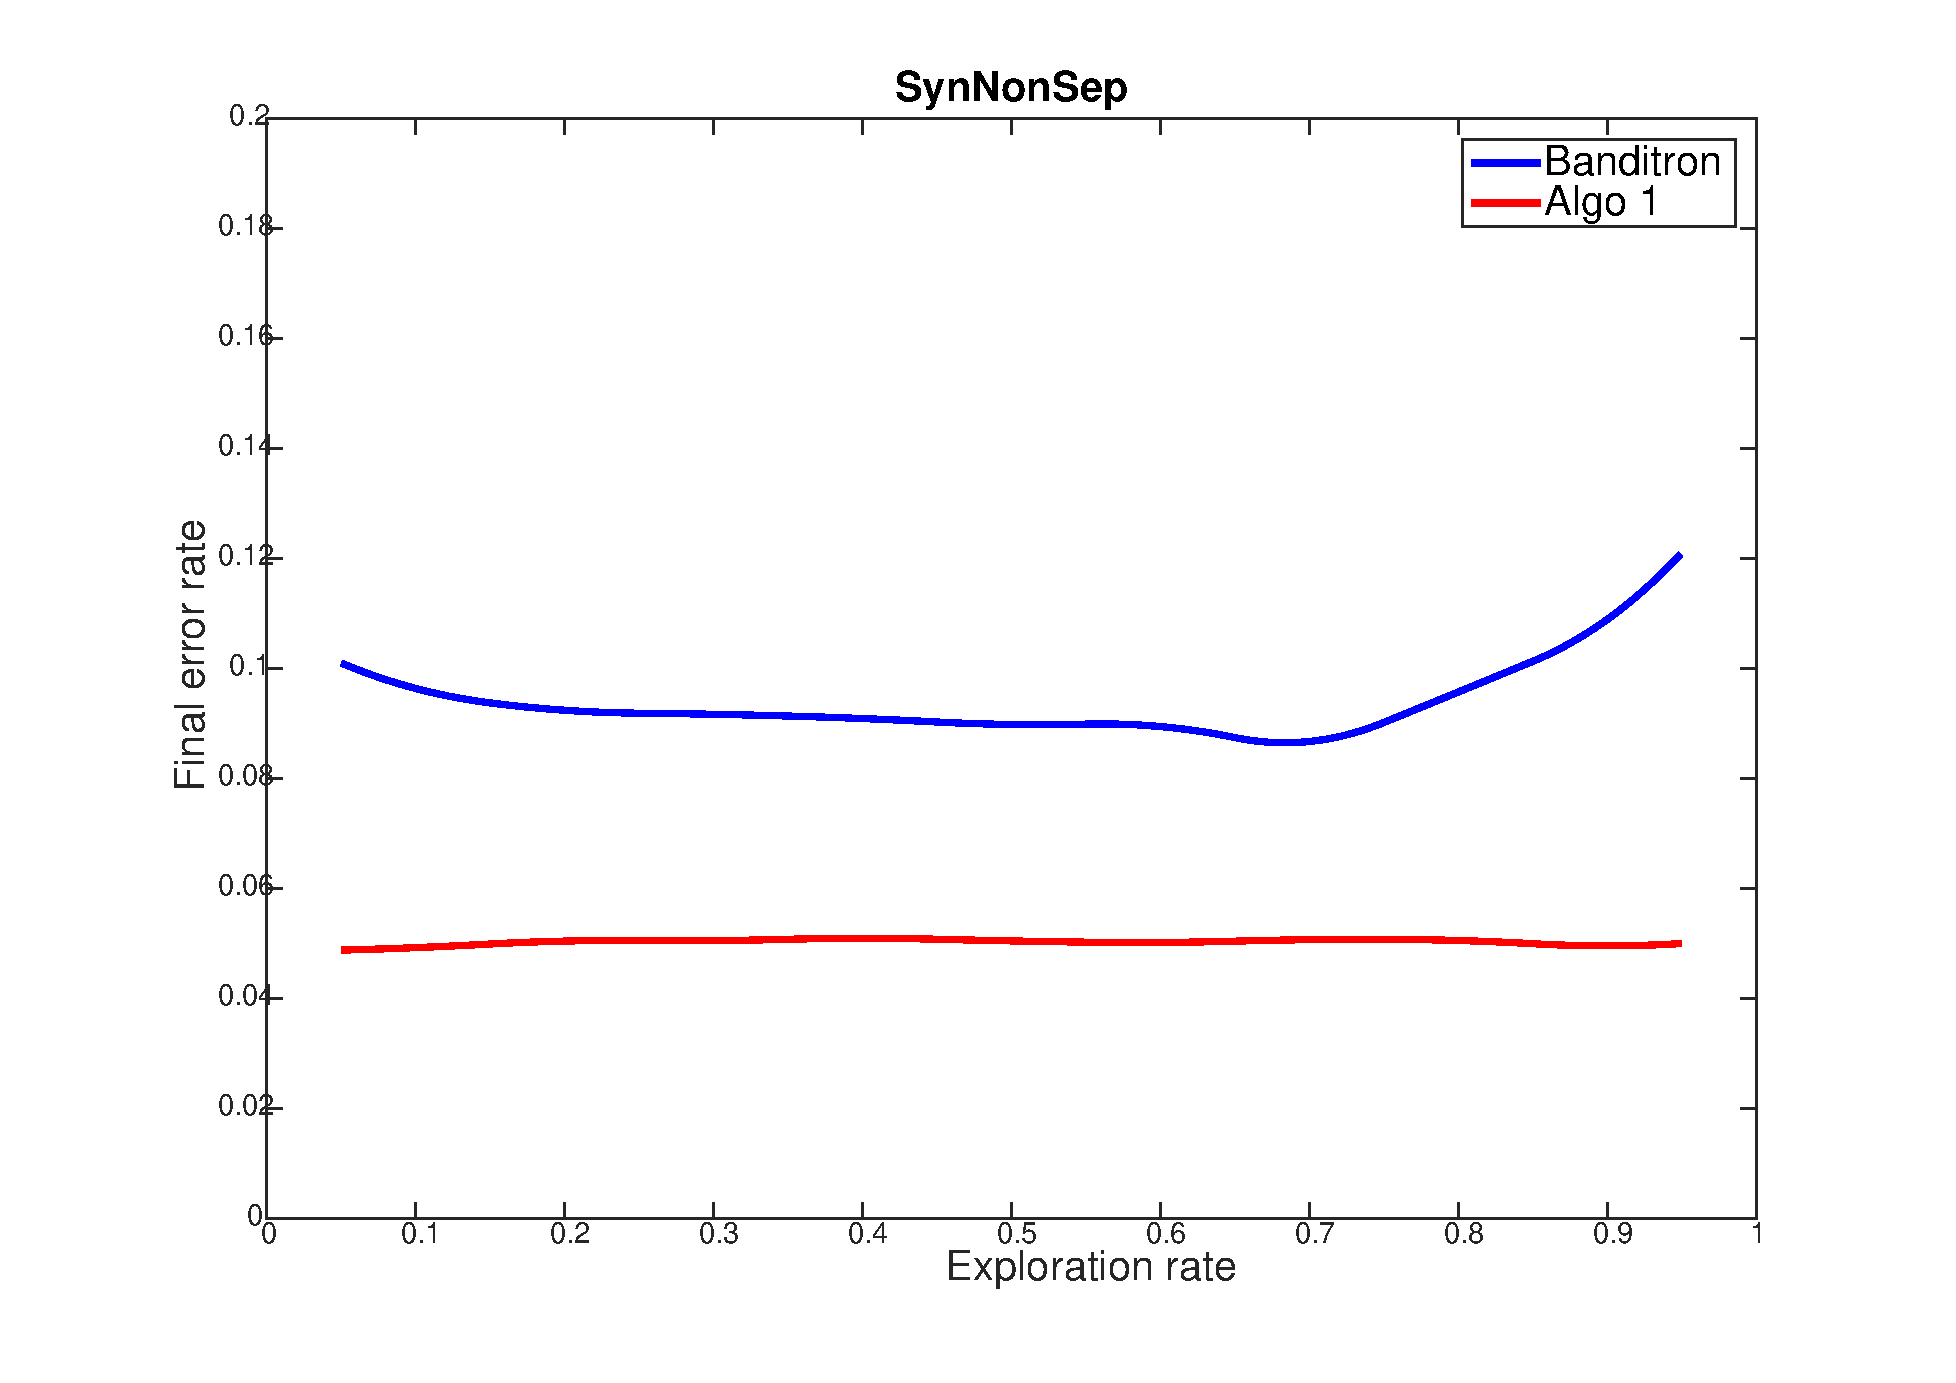
\includegraphics[width=.7\linewidth]{figs/SynNonSep_gamma.eps}}
	%\centerline{\bf (b)}
	\centerline{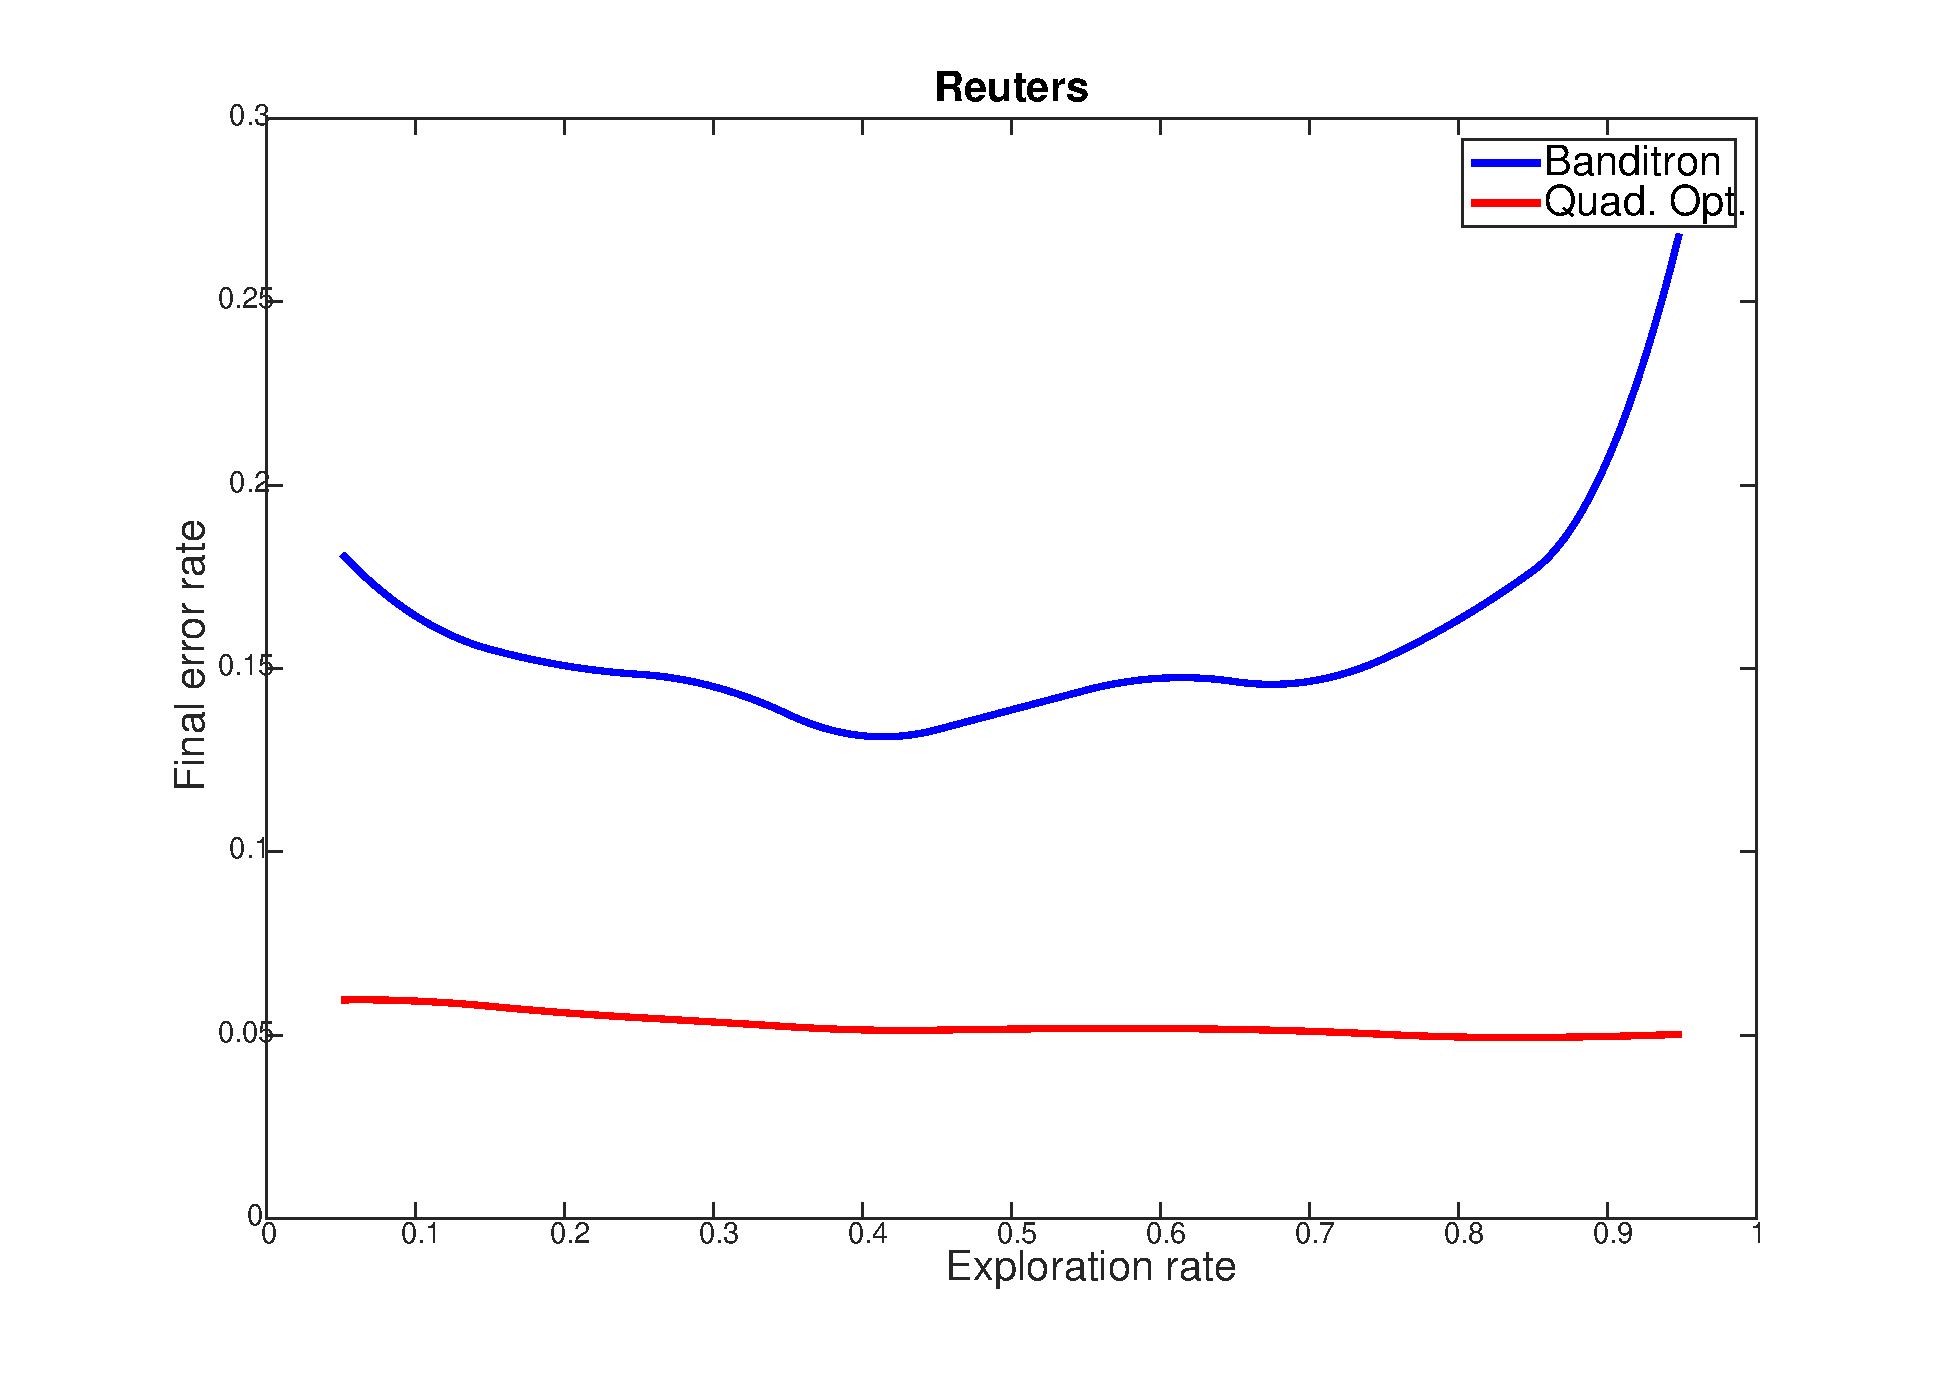
\includegraphics[width=.7\linewidth]{figs/Reuters_gamma.eps}}
	\caption{Banditron and one-Bit feedback Passive Aggressive (BPA) final error rate in function of the exploration rate $\varepsilon$, on SynNonSep (top) and Reuters (bottom) datasets. Parameters are in table 2.}
	\label{pic:BPASNSerr}
%\end{figure}

%\begin{figure}[ht!]
	
	%\caption{Taux d'erreur moyen du Banditron et du BPA en fonction du taux d'exploration $\varepsilon$ }
	%\label{pic:BPARCVerr}
\end{figure}

We investigate on Figure \ref{pic:BPASNSerr} %et  \ref{pic:BPARCVerr}  
the effect of the exploration parameter $\varepsilon$ on the final classification rate, for the Banditron and the one-Bit feedback Passive-Aggressive (algorithm \ref{algo:quad}). Apart from better final classification rate, the passive aggressive setup is shown insensitive to variable $\varepsilon$, on contrary to the Banditron having a known exploration rate dependence. Greedy exploitation and pure exploration show similar effectiveness in our case. In practice, this result allows consider decreasing exploration rates over learning sessions, for to take advantage of the classification rates attained in the course of learning. 

%présentent l'effet du paramètre d'exploration $\varepsilon$ sur les taux d'erreur obtenus en fin de session par le Banditron et le BPA, sur les bases SynNonSep et Reuters. Contrairement au Banditron, le taux de réussite du BPA est remarquablement insensible à la valeur de $\varepsilon$. Autrement dit, les performances d'apprentissage sont les mêmes pour un $\varepsilon$ faible que pour un $\varepsilon$ élevé. Ce résultat permet d'envisager la mise en place de politiques à taux d'exploration variable, afin de de profiter en fin d'apprentissage des bonnes performances du classifieur.
%Par ailleurs, dans les deux cas, le taux d'erreurs obtenu par BPA en fin de session est plus faible que celui du Banditron. 


%\begin{figure}[h!]

%	\centerline{
%		\includegraphics[width=\linewidth]{figs/regret.eps}
%	}
%	\caption{Regret estimé sur le jeu de données Reuters pour l'algorithme BPA}
%	\label{pic:regret}
%\end{figure}

%La figure \ref{pic:regret} donne une estimation du regret cumulé sur la base Reuters pour les 20000 premiers exemplaires, pour l'algorithme BPA, en utilisant pour la comparaison le classifieur obtenu en fin de session. On observe un taux de croissance du regret cumulé sous-linéaire, compatible avec la prédiction $O(\sqrt{t})$ (voir théorème 2). 


\begin{figure}[htp]
	
	\centerline{
		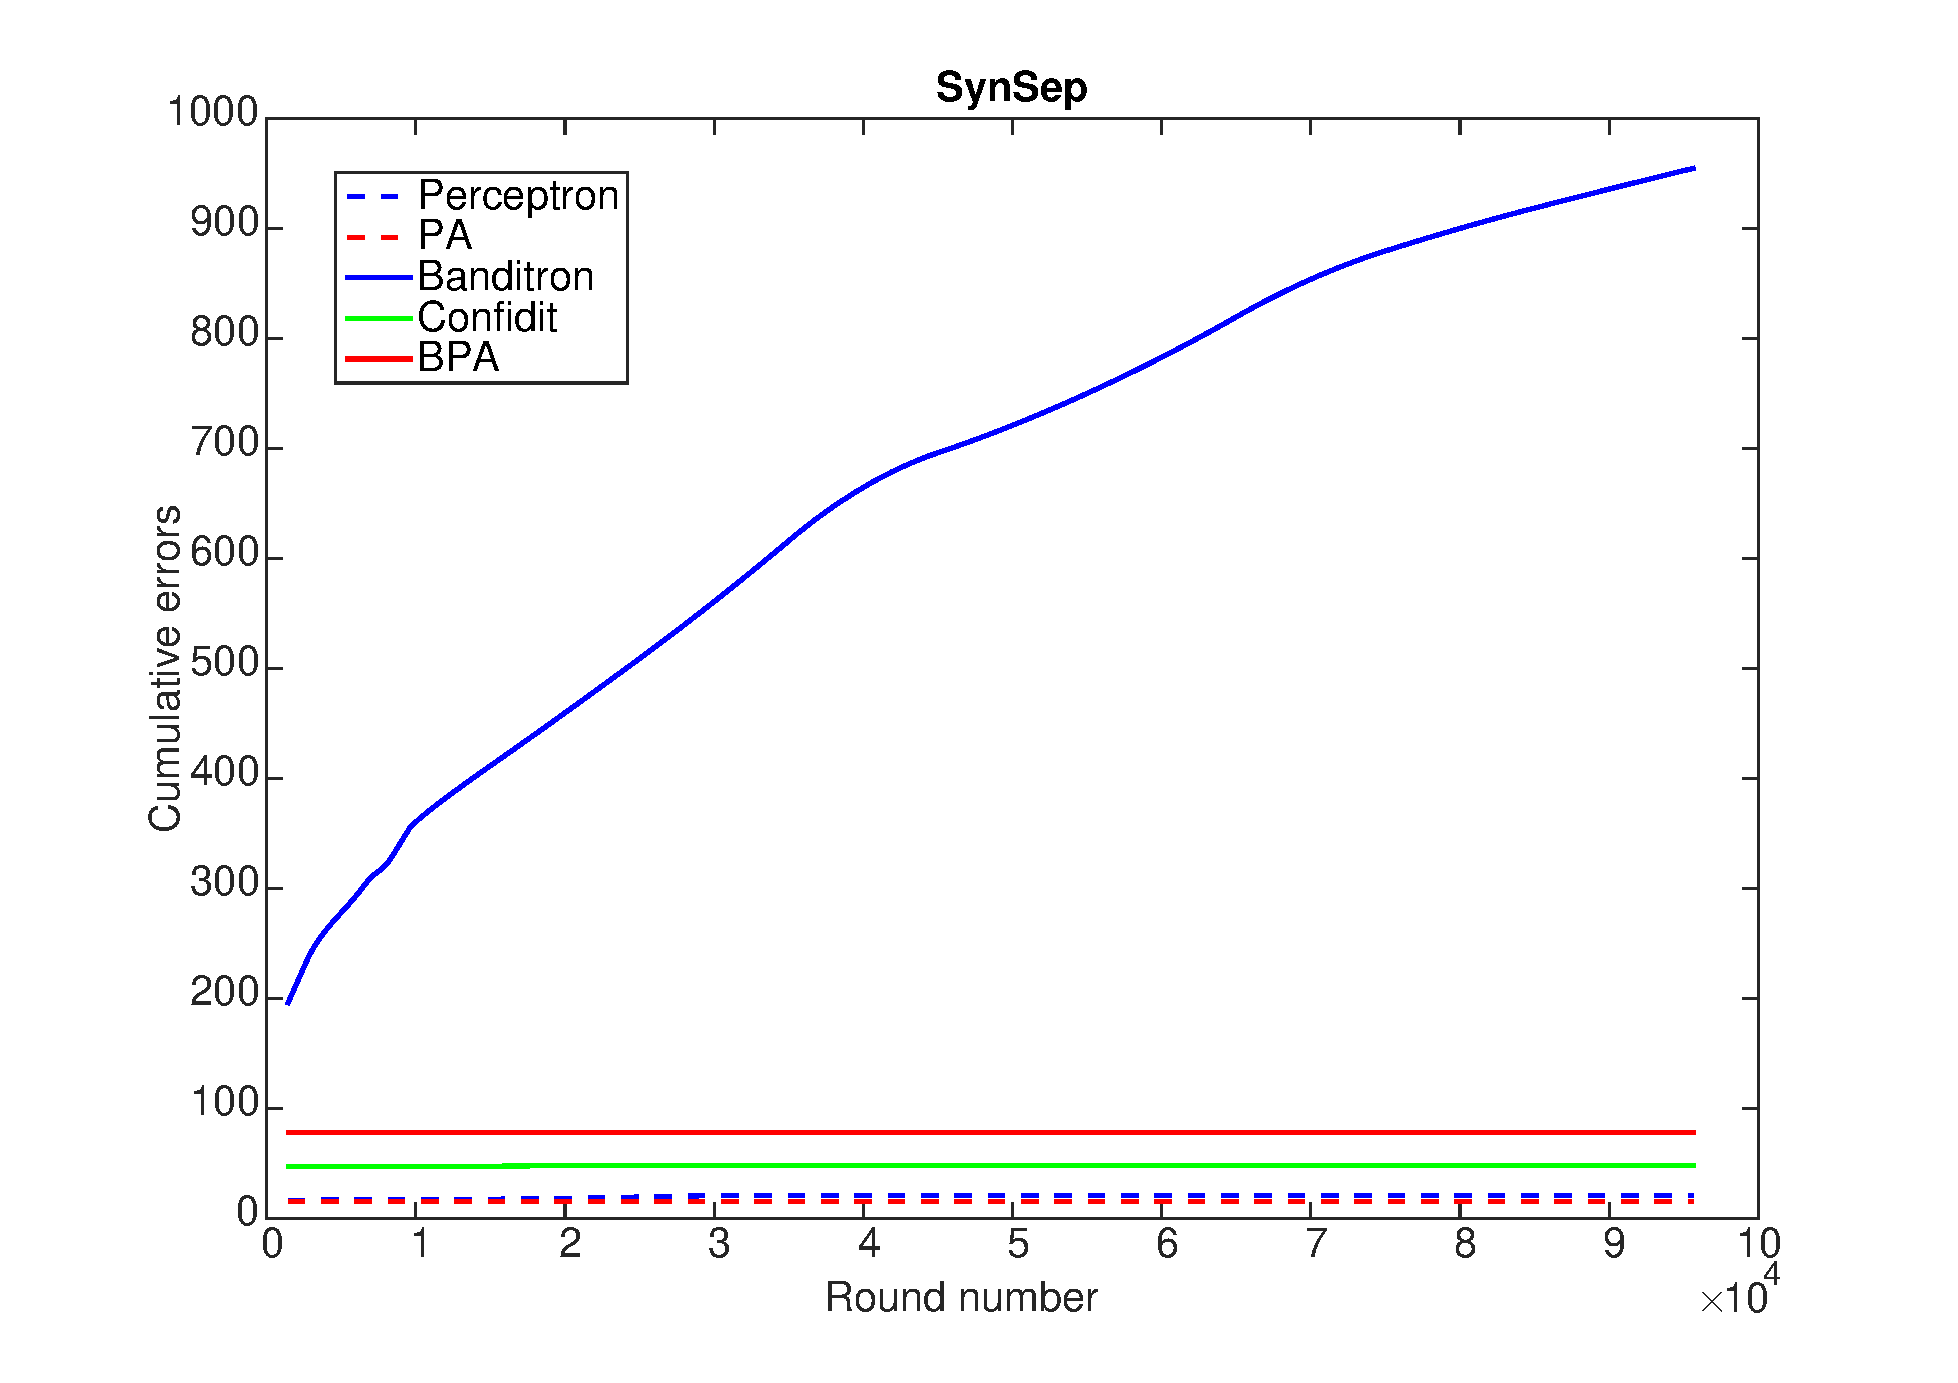
\includegraphics[width=.6\linewidth]{figs/SynSep.eps}
	}
	
	\centerline{
		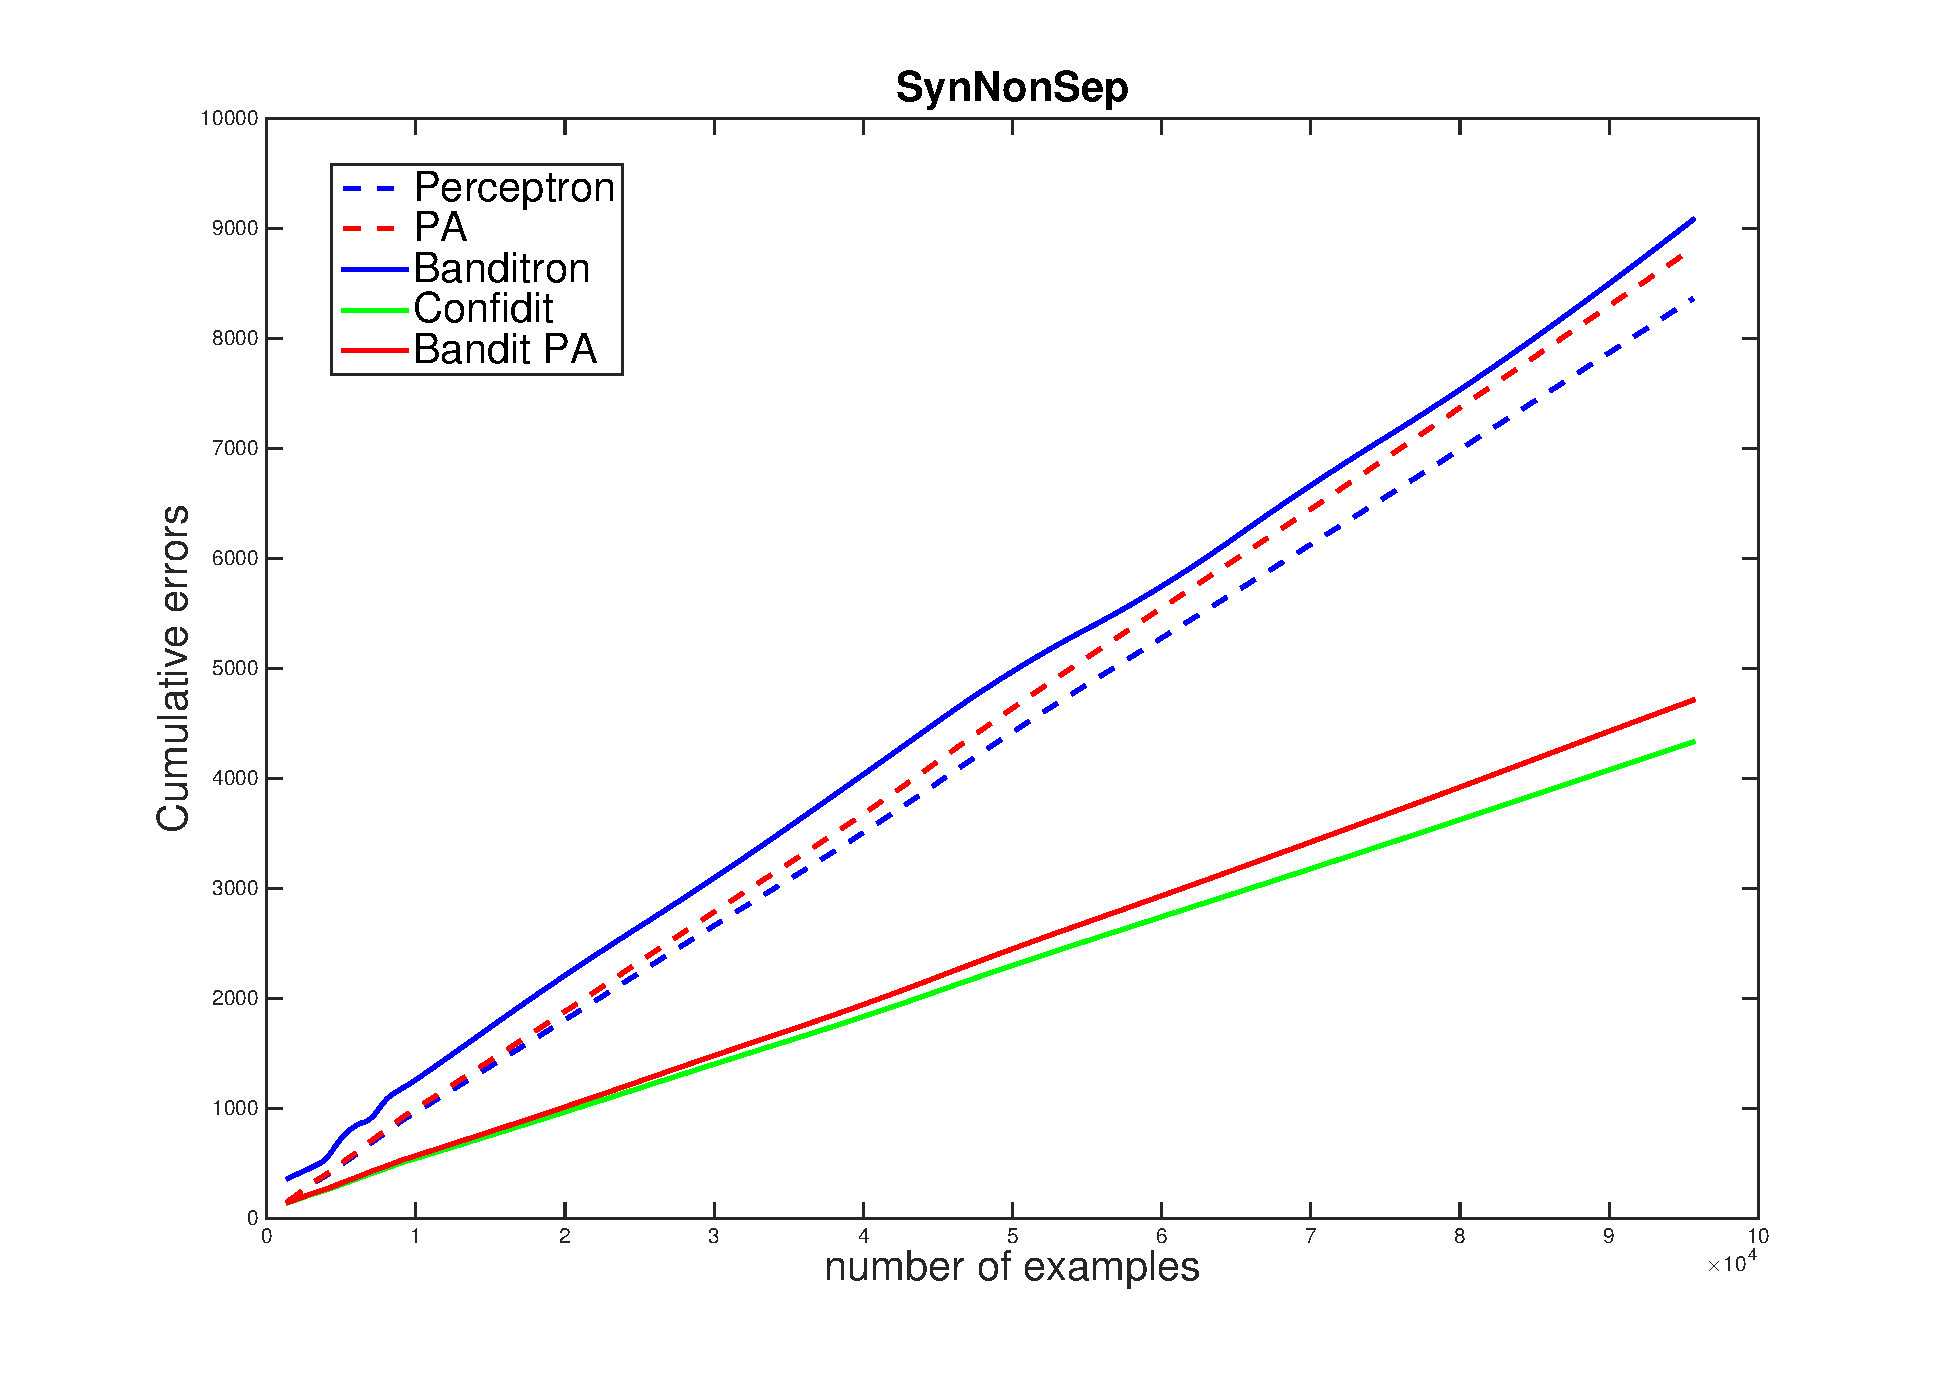
\includegraphics[width=.6\linewidth]{figs/SynNonSep.eps}
	}
	\centerline{
		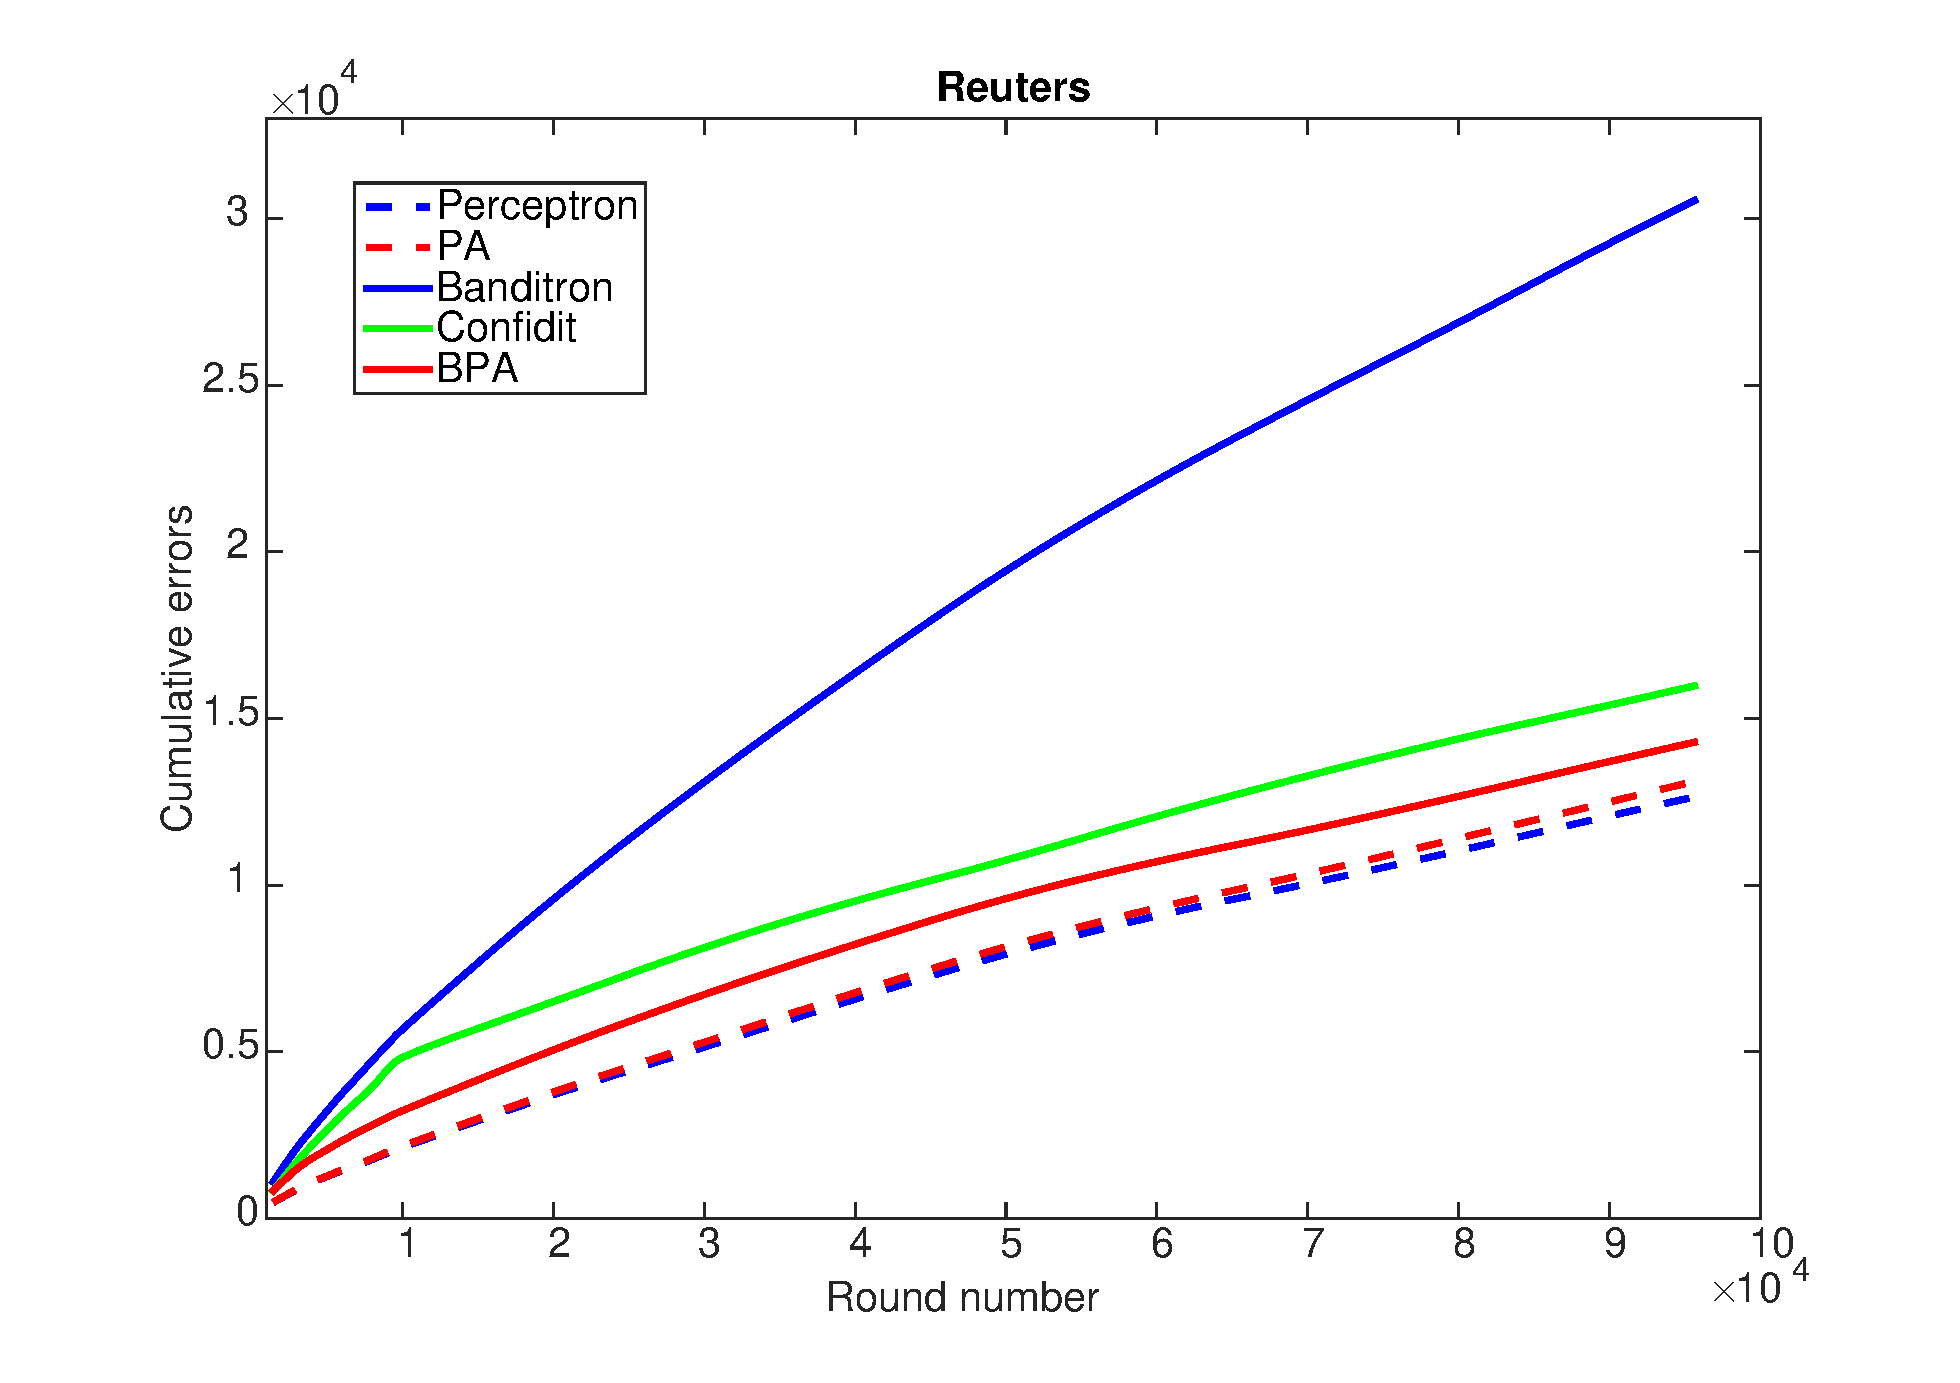
\includegraphics[width=.6\linewidth]{figs/RCV1_v2_53class.eps}}
	\caption{Perceptron, Passive-Aggressive (PA), Banditron, Confidit and one-Bit feedback Passive Aggressive (BPA) cumulative errors  over trial number for the SynSep (9 classes), SynNonSep (9 classes) and Reuters (53 classes) databases. Parameters are in table 2.}
	\label{pic:BPASS}
\end{figure}

The Perceptron, Passive-Aggressive (PA), Banditron, Confidit and one-Bit feedback Passive Aggressive (BPA) cumulative errors are compared on figure \ref{pic:BPASS} over the SynSep, SynNonSep and Reuters RCV1-v2 datasets. 

The first dataset being linearly separable, a final error bound is rapidly attained by all methods except for the Banditron showing only a monotonic decrease of the error rate. The convergence is shown even faster for the supervised methods (Perceptron and PA), for barely 20 errors are observed over $10^5$ instances. 

%Sur le premier jeu synthétique et linéairement séparable, on constate que la borne est rapidement atteinte pour Perceptron, PA, Confidit et BPA. Seul Banditron présente une courbe croissante qui ne permet pas de borner le taux d'erreurs cumulées.  On constate également, comme prévu, un taux d'erreur total plus faible pour les algorithmes supervisés que pour les algorithmes à feedback de Bandit.

In the SynNonSep case, as the  5\% label noise is irreductible, all methods show a linear growth of the cumulative error. However, the slower increase seen on Confidit and BPA  point out a better resilience to label noise, when compared to the supervised setup. This resilience, that was noticed in \cite{crammer2013multiclass} and \cite{ngo2013upper}, thus extends here to the BPA approach.

%\textcolor{red}{OK-- Il manque les valeurs des paramètres pour les différents algorithmes (faire un tableau comme dans la partie précédente).}

The Reuters RCV1-v2 database provides a  scale-realistic testbed.
% allowing to highlight the BPA setup effectiveness. 
The sub-linear cumulative error rate  shown by all methods indicate that learning is effective in all case, with, however, a clear gap between the Banditron and the other methods. In detail, the two supervised algorithms outperform by little BPA, followed by Confidit, and then the Banditron far behind. The first four methods show almost similar final slopes, on contrary to the Banditron showing a higher final error rate (see figure \ref{pic:BPASNSerr}). The good performances of BPA and Confidit are noticeable here, for the number of classes is high (53) and the labelling information consequently very scarce. 
Moreover, the marked prevailing of BPA over Confidit is also noticeable for its algorithmic complexity is much less\footnote{Confidit uses a second order sample covariance estimate, this covariance matrix being reduced  to a mere diagonal in the high-dimensional case (see  \cite{crammer2013multiclass}).}. 

\begin{figure}[htp]

	\centerline{
		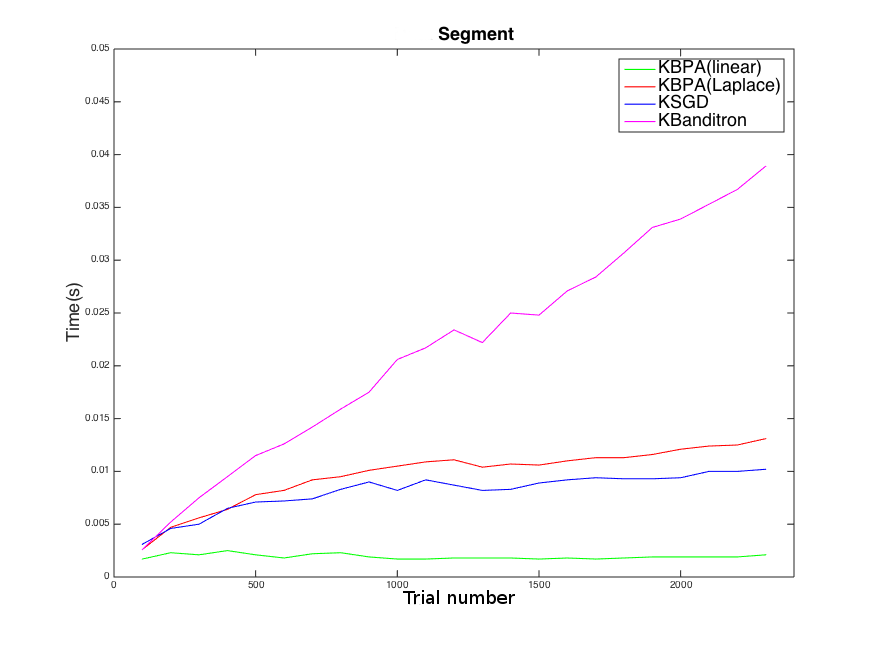
\includegraphics[width=.7\linewidth]{figs/Segment_kernel_T.png}}
	\centerline{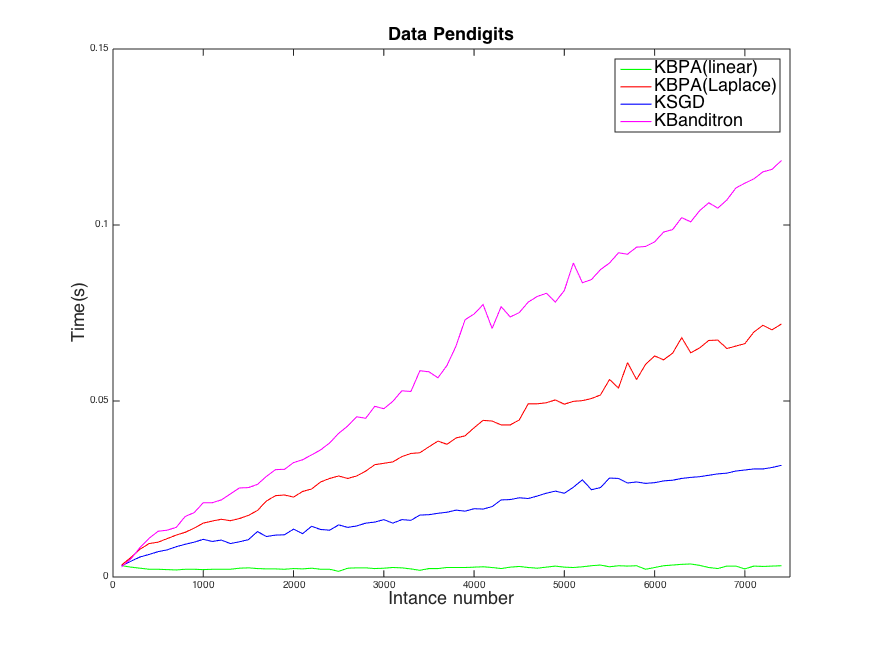
\includegraphics[width=.7\linewidth]{figs/Pendigits_kernel_T.png}}
\caption{Linear BPA (algorithm 1), kernel BPA (algorithm 1), kernel SGD (algorithm 2)  and kernel Banditron average computational cost over trial number on Segment (top) and Pendigits (bottom) databases. Parameters are in table 2.}
\label{pic:PKT}	
\end{figure}

The Segment and Pendigits datasets, to which Linear BPA, kernel BPA, kernel SGD and kernel Banditron are applied on figures \ref{pic:PKT} and \ref{pic:PKCM}, present a dramatic decrease in size, with vectors of only 19 features in Segment and only 16 in Pendigits.
These more reduced feature spaces are counterbalanced by a stronger non-separability, that dictates the use of kernel methods. 
Online learning with kernels being generally burdened by the increasing size of the prototype vectors set (see \cite{kivinen2004online}), we check here for the sparsity of the different setups. In particular, we compare the K-BPA native sparsity (algorithm \ref{algo:quad}) with the explicit sparsity control of the SGD method (algorithm \ref{algo:HGD}), while the linear BPA provides a baseline reference, and the kernel-Banditron illustrates the upper bound computational cost of a non-sparse update. 

%Sparse and conservative updates are thus preferred, for smaller prototype sets, and thus lesser computational costs, should be attained.  


The increasing computational cost over time is shown on figure \ref{pic:PKT}. Apart from the linear BPA baseline constant cost, all kernel-based setups show a monotonic increase over time, with the most parsimonious trend obtained by the K-SGD, followed by the K-BPA, and then the K-Banditron constant trend.  The computational cost of a learning session is consequently $0(T)$ for the linear BPA (best case), $O(T^2)$ for the K-Banditron (worst case) and in between for the two other cases. The BPA algorithm is expected to reach a constant cost after the final number of prototypes is reached, this number being set to 200 on the Segment database and 500  on the Pendigits one. A plateau is roughly observed after 1000 trials on the Segment database, while a continuing complexity rise is observed at slow rate in the other case. The K-BPA, while still more costly, shows a very close-by trend on the Segment database, and a more marked difference on the Pendigits database. These results confirm in general the sparsity effectiveness, and the subsequent reduced computational cost, of the K-BPA setup.


\begin{figure}[htp]
	
	\centerline{
	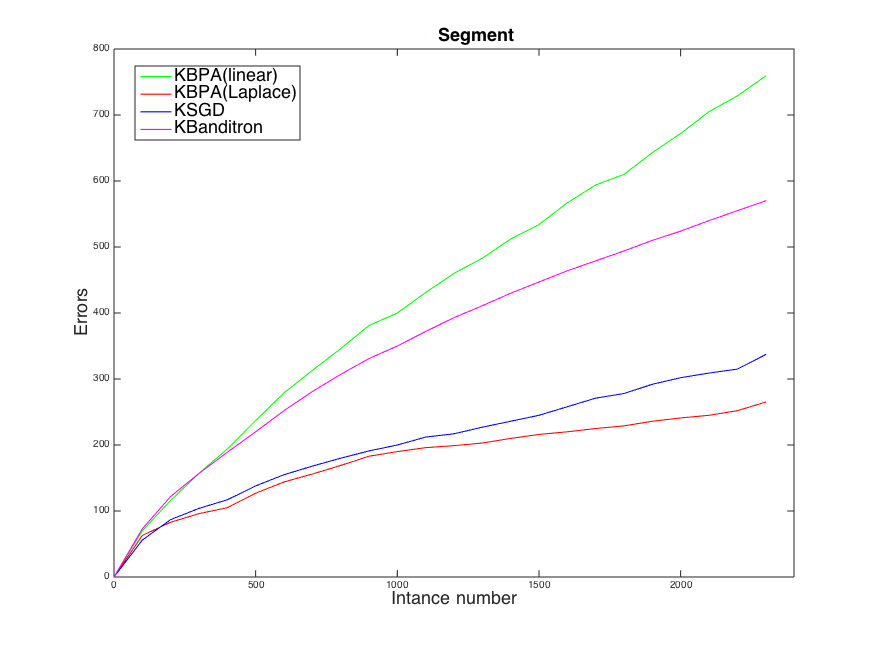
\includegraphics[width=.7\linewidth]{figs/Segment_kernel_CM.png}}
\centerline{
	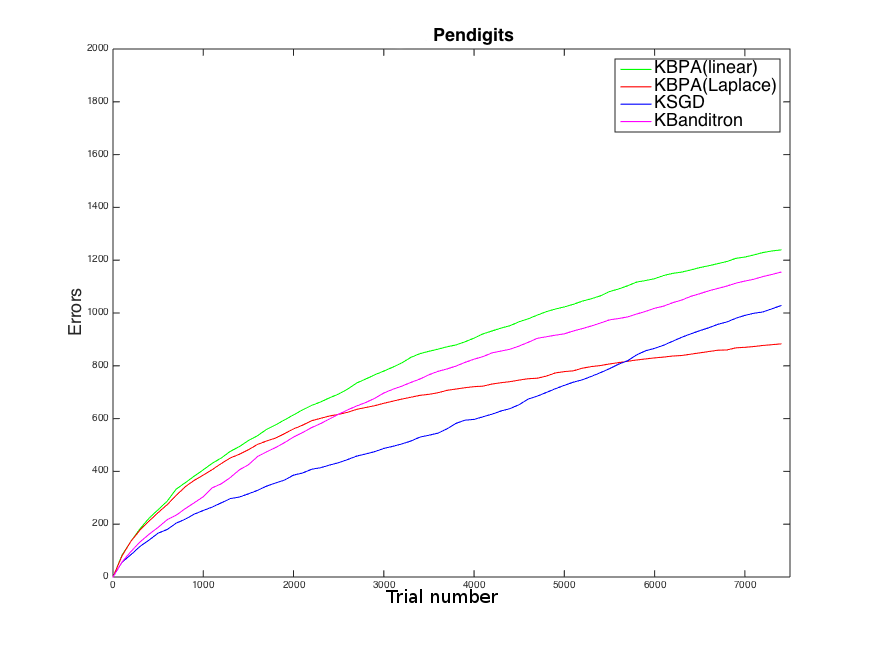
\includegraphics[width=.7\linewidth]{figs/Pendigits_kernel_CM.png}}
	\caption{Linear BPA (algorithm 1), kernel BPA (algorithm 1), kernel SGD (algorithm 2)  and kernel Banditron cumulative errors over trial number on Segment  (top) and Pendigits(bottom)  databases. Parameters are in table 2.}
	\label{pic:PKCM}
\end{figure}

%\begin{figure}[h!]
%	\centerline{
%		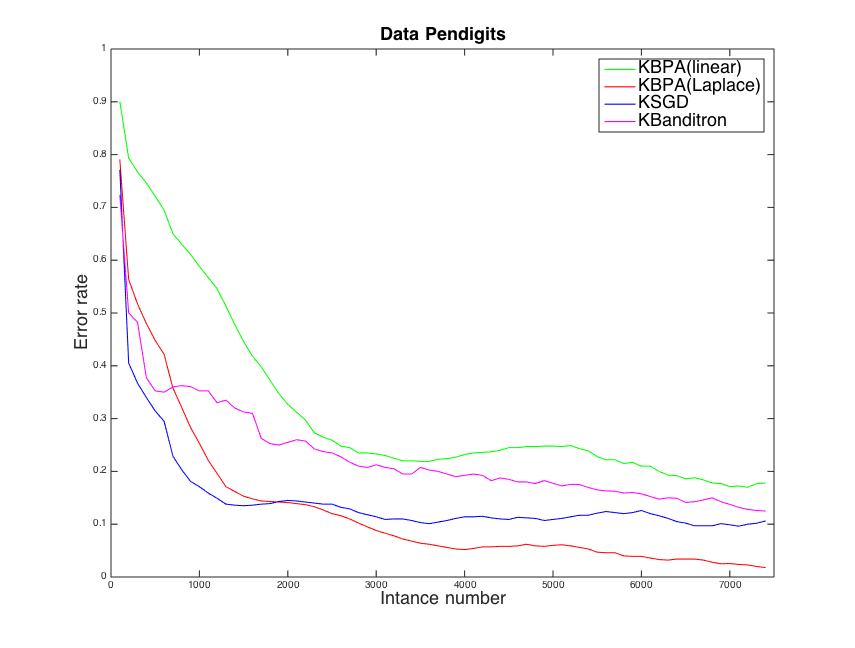
\includegraphics[width=\linewidth]{figs/Pendigits_kernel_M.png}}
%	\caption{Average error rate for each instance of Data Pendigits}
%	\label{pic:PKM}
%\end{figure}

%\begin{figure}[t!]
	
%	\caption{Cumulative Errors of Data Segment}
%	\label{pic:SKCM}
%\end{figure}

%\begin{figure}[h!]
%	\centerline{
%		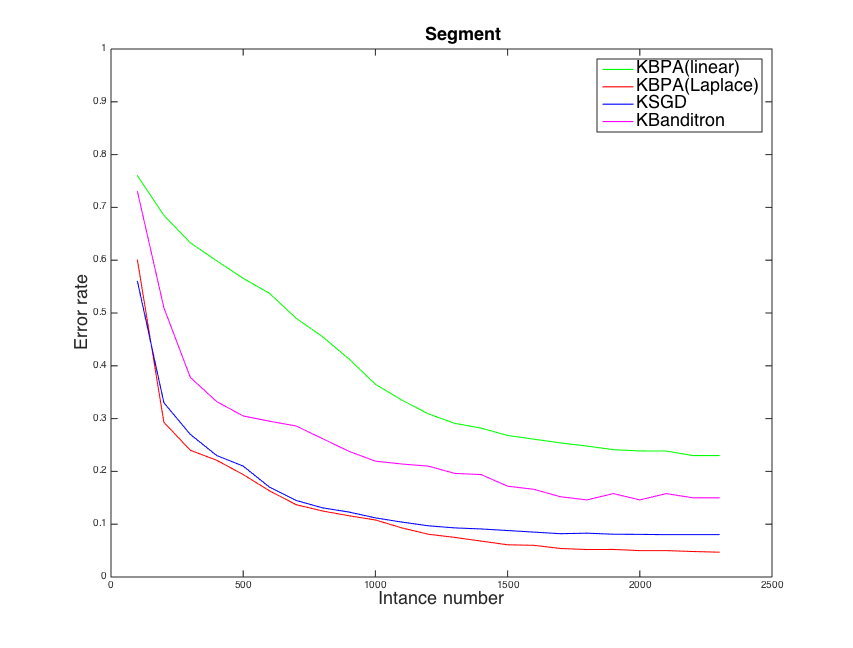
\includegraphics[width=\linewidth]{figs/Segment_kernel_M.png}}
%	\caption{Average error rate for each instance of Data Segment}
%	\label{pic:SKM}
%\end{figure}

Now turning to the classification rates, the cumulative errors obtained by the linear BPA, kernel BPA, kernel SGD and kernel Banditron on the Segment and Pendigits databases are shown on figure~\ref{pic:PKCM}. %, \ref{pic:PKM}, 
%et \ref{pic:SKCM} 
%et \ref{pic:SKM}  
The first thing to be noticed is the prevailing of the Kernel setups over the linear one in both cases, and particularly on the Segment database where the linear BPA hardly shows improvement over time. 
 The banditron is generally close to this worst-case scenario, while the K-SGD, despite a good initial startup, experience difficulty to capitalize improvement over time (more particularly on the Pendigits case). In contrast, the kernel BPA is clearly found to outperform the other methods, in particular  regarding the final error rate: the final less than 2\% error rate obtained on the Pendigits database (not shown) overtakes the other methods, but also approaches the state-of-the-art classification rates obtained in offline/full feedback settings. 


%présentent enfin les taux d'erreur moyens et cumulés produits par ces différents algorithmes au cours de l'apprentissage des bases Segment and Pendigits. Les courbes d'erreurs cumulées mettent en évidence dans ce cas de l'approche à noyaux sur l'approche linéaire, du fait du caractère non-linéairement séparable des données utilisées. Par ailleurs, l'algorithme BPA présente dans les deux cas les meilleurs performances d'apprentissage que l'algorithme du Banditron. L'algorithme KSGD présente de bonnes performances en début d'apprentissage, mais tend ensuite à atteindre un plateau de performances (du fait de la troncature) tandis que BPA présente une amélioration plus régulière lui permettant de dépasser les performances de KSGD en fin de session. On constate en particulier des taux d'erreurs très faibles en fin de session pour la base Pendigit. Ces performances d'apprentissage sont remarquables du fait de l'absence d'information de classification complète.  

%\begin{figure}[h!]
%\label{pic:PKR}
%\centerline{
%\includegraphics[scale = 0.4]{fig05/mc/Pendigits_kernel_R.png}}
%\caption{Cumulative loss of Data Pendigits}
%\end{figure}







%\subsection{High-dimensional datassets}
%\label{subsec:BPAE}
%Here, we evaluate the algorithms over two synthetic and three real world data sets. Their characteristics are summarized in Table~\ref{table:mce}.
%
%\begin{table}[h]
%	\caption{Summary of the three high-dimensional datasets, including the numbers of instances, features, labels and whether the number of examples in each class are balanced.}
%	\label{table:mce}
%	\begin{center}
%		\begin{tabular}{l l l l l}
%			{\bf Dataset}  & {\bf Instances} & {\bf Features} & {\bf Labels}& {\bf Balanced}\\
%			\hline
%			SynSep & $10^5$ 	& 400 	& 9 & Y\\
%			
%			SynNonSep & $10^5$ & 400 	& 9 & Y\\
%			
%			RCV1-v2  & $10^5$ 	& 47236 	& 53 & N\\
%			
%			%Letter 	&$2*10^4$	&16	&26	&N\\
%			
%			%Pen-Based &$1.32*10^4$	&16	&10	&N\\
%		\end{tabular}
%	\end{center}
%\end{table}
%
%\textbf{Data sets}:
%The first data set, denoted by SynSep,  is a 9-class, 400-dimensional synthetic data set of size $10^5$. More details about the method to generate this data set can be found in \cite{kakade2008efficient}. The SynSep  idea is to have a simple simulation of generating a text document. The coordinates represent different words in a small vocabulary of size $400$. We ensure that SynSep is linearly separable. 
%
%The second data set, denoted by SynNonSep, is constructed  the same way as  SynSep except that a 5\% label noise is introduced, which makes the data set non-separable. 
%
%The third data set is collected from the Reuters RCV1-v2 collection\cite{David04RCV}. The original data set is composed by multi-label instances. So we make some preprocessing likes \cite{RB08a}. First, its label hierarchy is reorganized by mapping the data set to the second level of RCV1 topic hierarchy. The documents that have labels of the third or forth level only are mapped to their parent category of the second level; Second, all multi-labelled instances have been removed. This RCV1-v2 is a 53-class,  47236-dimensional real data set of size $10^5$. 
%
%%The fourth and fifth data sets are collected from \cite{letter26SC,number10SC}. The fourth data set is to identify each of a large number of black-and-white rectangular pixel displays as one of the 26 capital letters in the English alphabet. The character images were based on 20 different fonts and each letter within these 20 fonts was randomly distorted to produce a file of 20000 unique stimuli. Each stimuli was converted into 16 primitive numerical attributes (statistical moments and edge counts). It forms a 26-class, 16-dimensional real data set of size $20000$. The fifth data set is a digit data base made by collecting 250 samples from 44 writers, using only (x,y) coordinate information represented as constant length feature vectors, which were resampled to 8 points per digit (therefore the data set contains 8 points $\times$ 2 coordinates = 16 features). This one is a 10-class, 16-dimensional real data set of size $10992$.
%
%\textbf{Results}
%Figures \ref{pic:BPASS} and~\ref{pic:BPASNS} show the experimental results on two synthetic data sets. For SynSep, a separable linear data set, all algorithms except Banditron obtain a good performance; with the non-separable SynNonSep data, Confidit and BPA outperform the other algorithms, even the supervised algorithms.  To different datasets, the parameters of different algorithms refer to Table~\ref{table:bpa}.
%\begin{table}[h]
%	\caption{The summary of algorithm parameters for different datasets. P. denotes Perceptron, PA is Passive-Aggressive online algorithm, B. is Banditron, C. is Confidit and BPA.}
%	\label{table:bpa}
%	\begin{center}
%		\begin{tabular}{lllllll}
%			{\bf Dataset}  & {\bf P.} & {\bf PA } & {\bf B.}& {\bf C.} & {\bf BPA}\\
%			\hline
%			SynSep & null & $C=0$ & $\varepsilon = 0.014$ &$\eta = 10^3$ & $\varepsilon = 0.4,C = 0$\\
%			
%			SynNonSep & null & $C=10^{-2}$ & $\varepsilon =0.65$ & $\eta = 10^3$& $\varepsilon = 0.8,C = 10^{-2}$\\
%			
%			Reuters & null & $C=10^{-2}$ & $\varepsilon =0.4$ & $\eta = 10^2$ & $\varepsilon = 0.2,C = 10^{-2}$\\
%			
%			%LR(26 letters) & null &  $C=0.1$ & $\varepsilon = 0.2$& $\eta=10^2$ & $\varepsilon = 0.8,C= 1$ \\
%			
%			%LR(10 numbers) & null & $C=0.1$ & $\varepsilon= 0.4$& $\eta = 10$ & $\varepsilon = 0.6,C=1$\\
%			
%		\end{tabular}
%	\end{center}
%\end{table}
%
%%\textcolor{red}{OK-- Il manque les valeurs des paramètres pour les différents algorithmes (faire un tableau comme dans la partie précédente).}
%
%Figure~\ref{pic:BPARCV} %, ~\ref{pic:BPALR10} and~\ref{pic:BPALR26} 
%presents the result on the real dataset. With this dataset, the supervised algorithms, despite their competitive advantage with respect to the ones with bandit feedback, do not significantly depart from BPA and Confidit, with classification results that clearly outperform Banditron. While having a lower computational complexity, BPA approach is even found to outperform Confidit in the most challenging situation, i.e. the high-dimensional case with a large number of classes (RCV1-v2 data set).
%
%The $\epsilon$ parameter represents the exploration rate in Banditron and BPA algorithms. We compare on Figure 3 the average error rates obtained on the two algorithms for different values of $\epsilon$ on the different data sets. In contrast with Banditron, BPA shows that $\epsilon$ has a very little influence on the final error rate, indicating a capability to deal with small exploration rates.
%
%
%\begin{figure}[h!]
%	
%	\centerline{
%		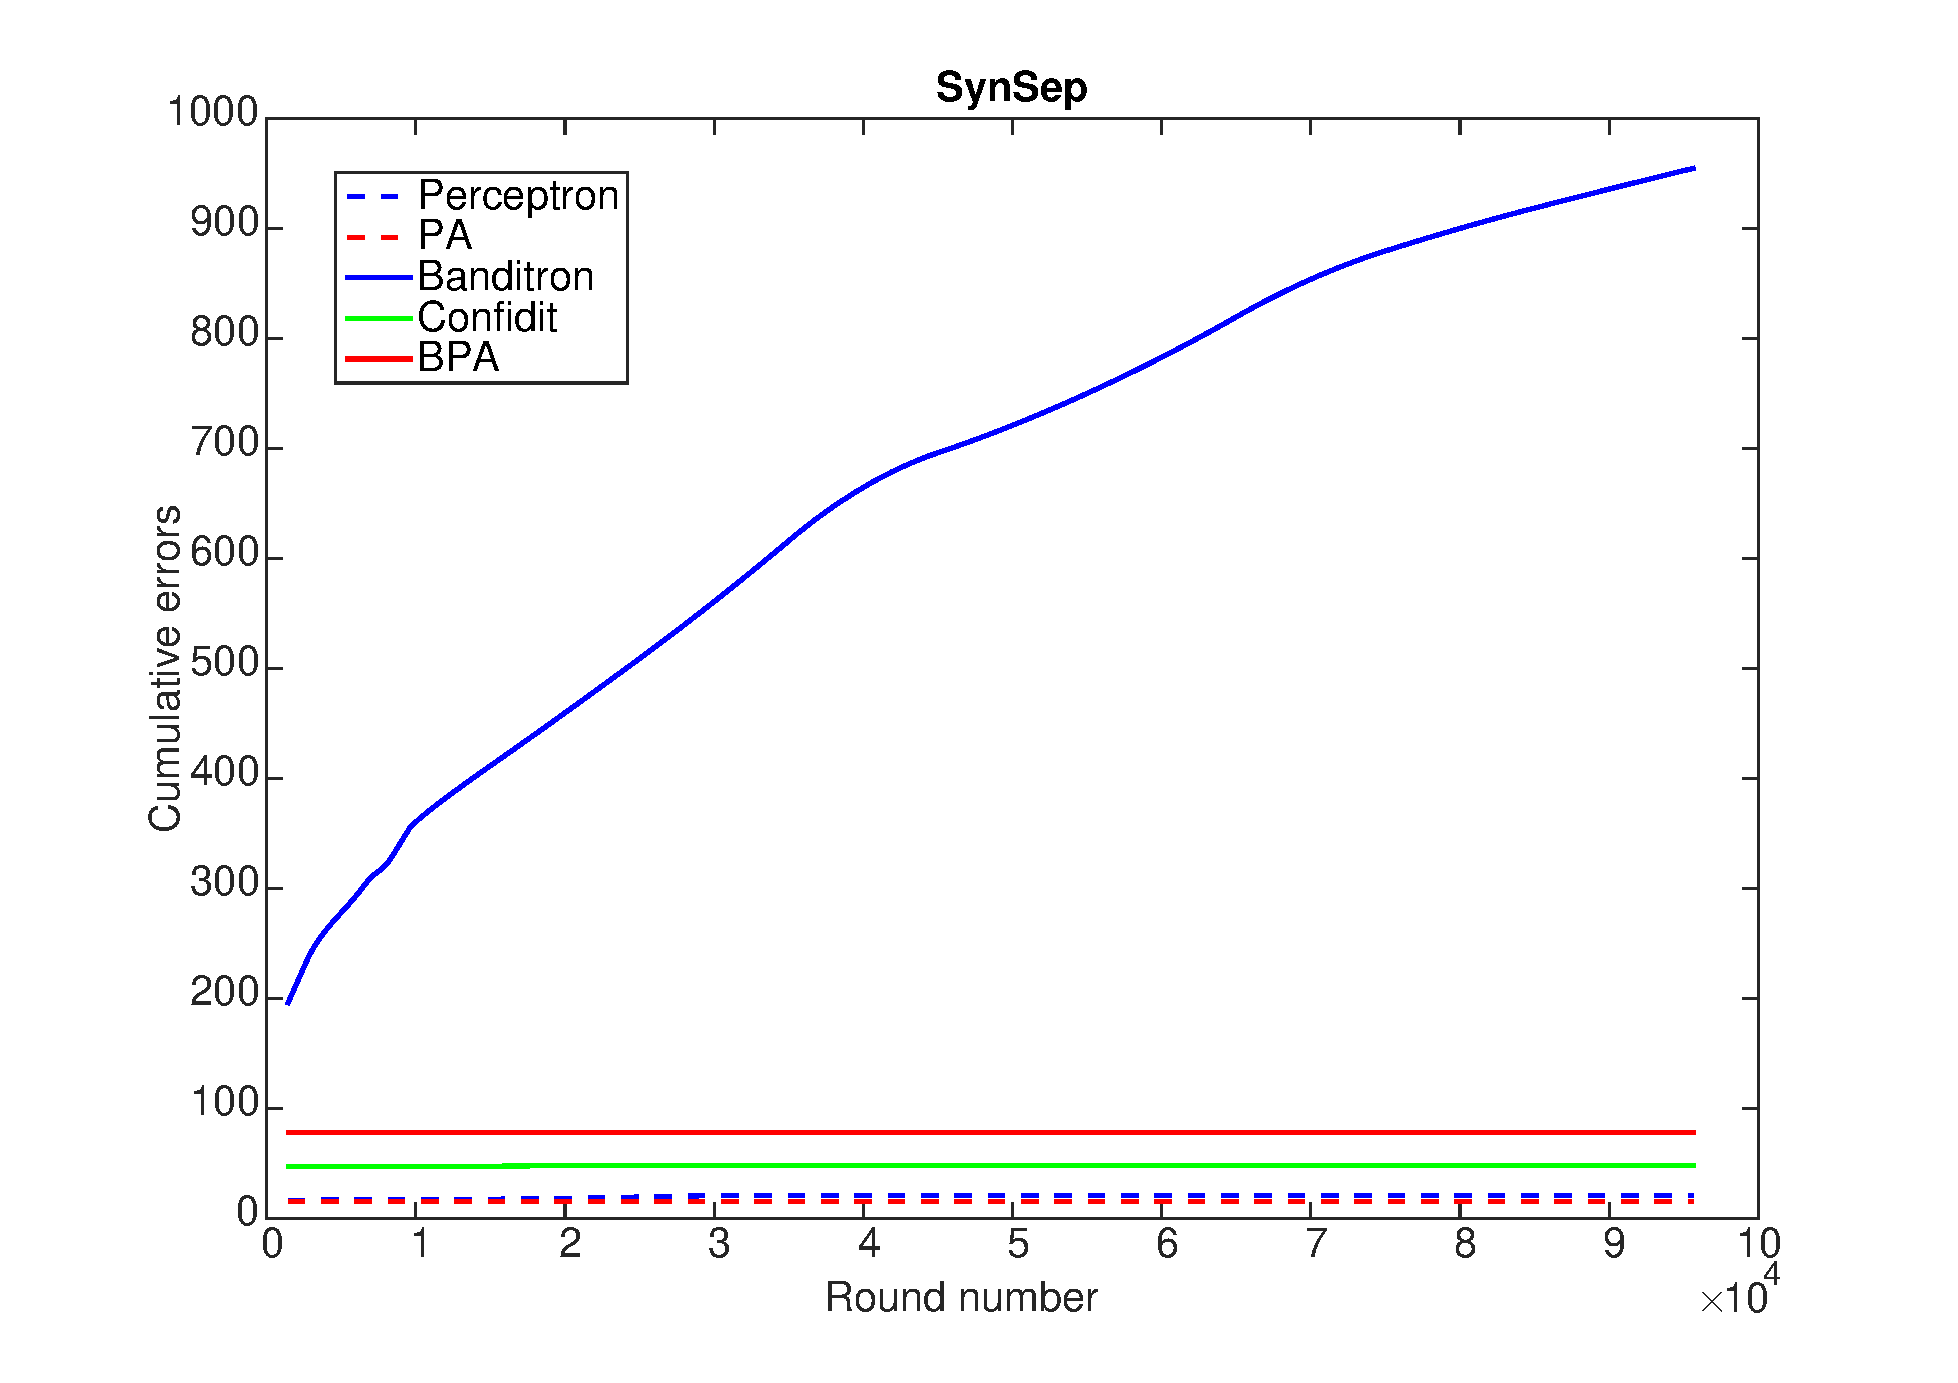
\includegraphics[scale = 0.4]{figs/SynSep.eps}
%	}
%	\caption{Cumulative Errors on the synthetic data set of  SynSep.}
%	\label{pic:BPASS}
%\end{figure}
%\begin{figure}[h!]
%	
%	\centerline{
%		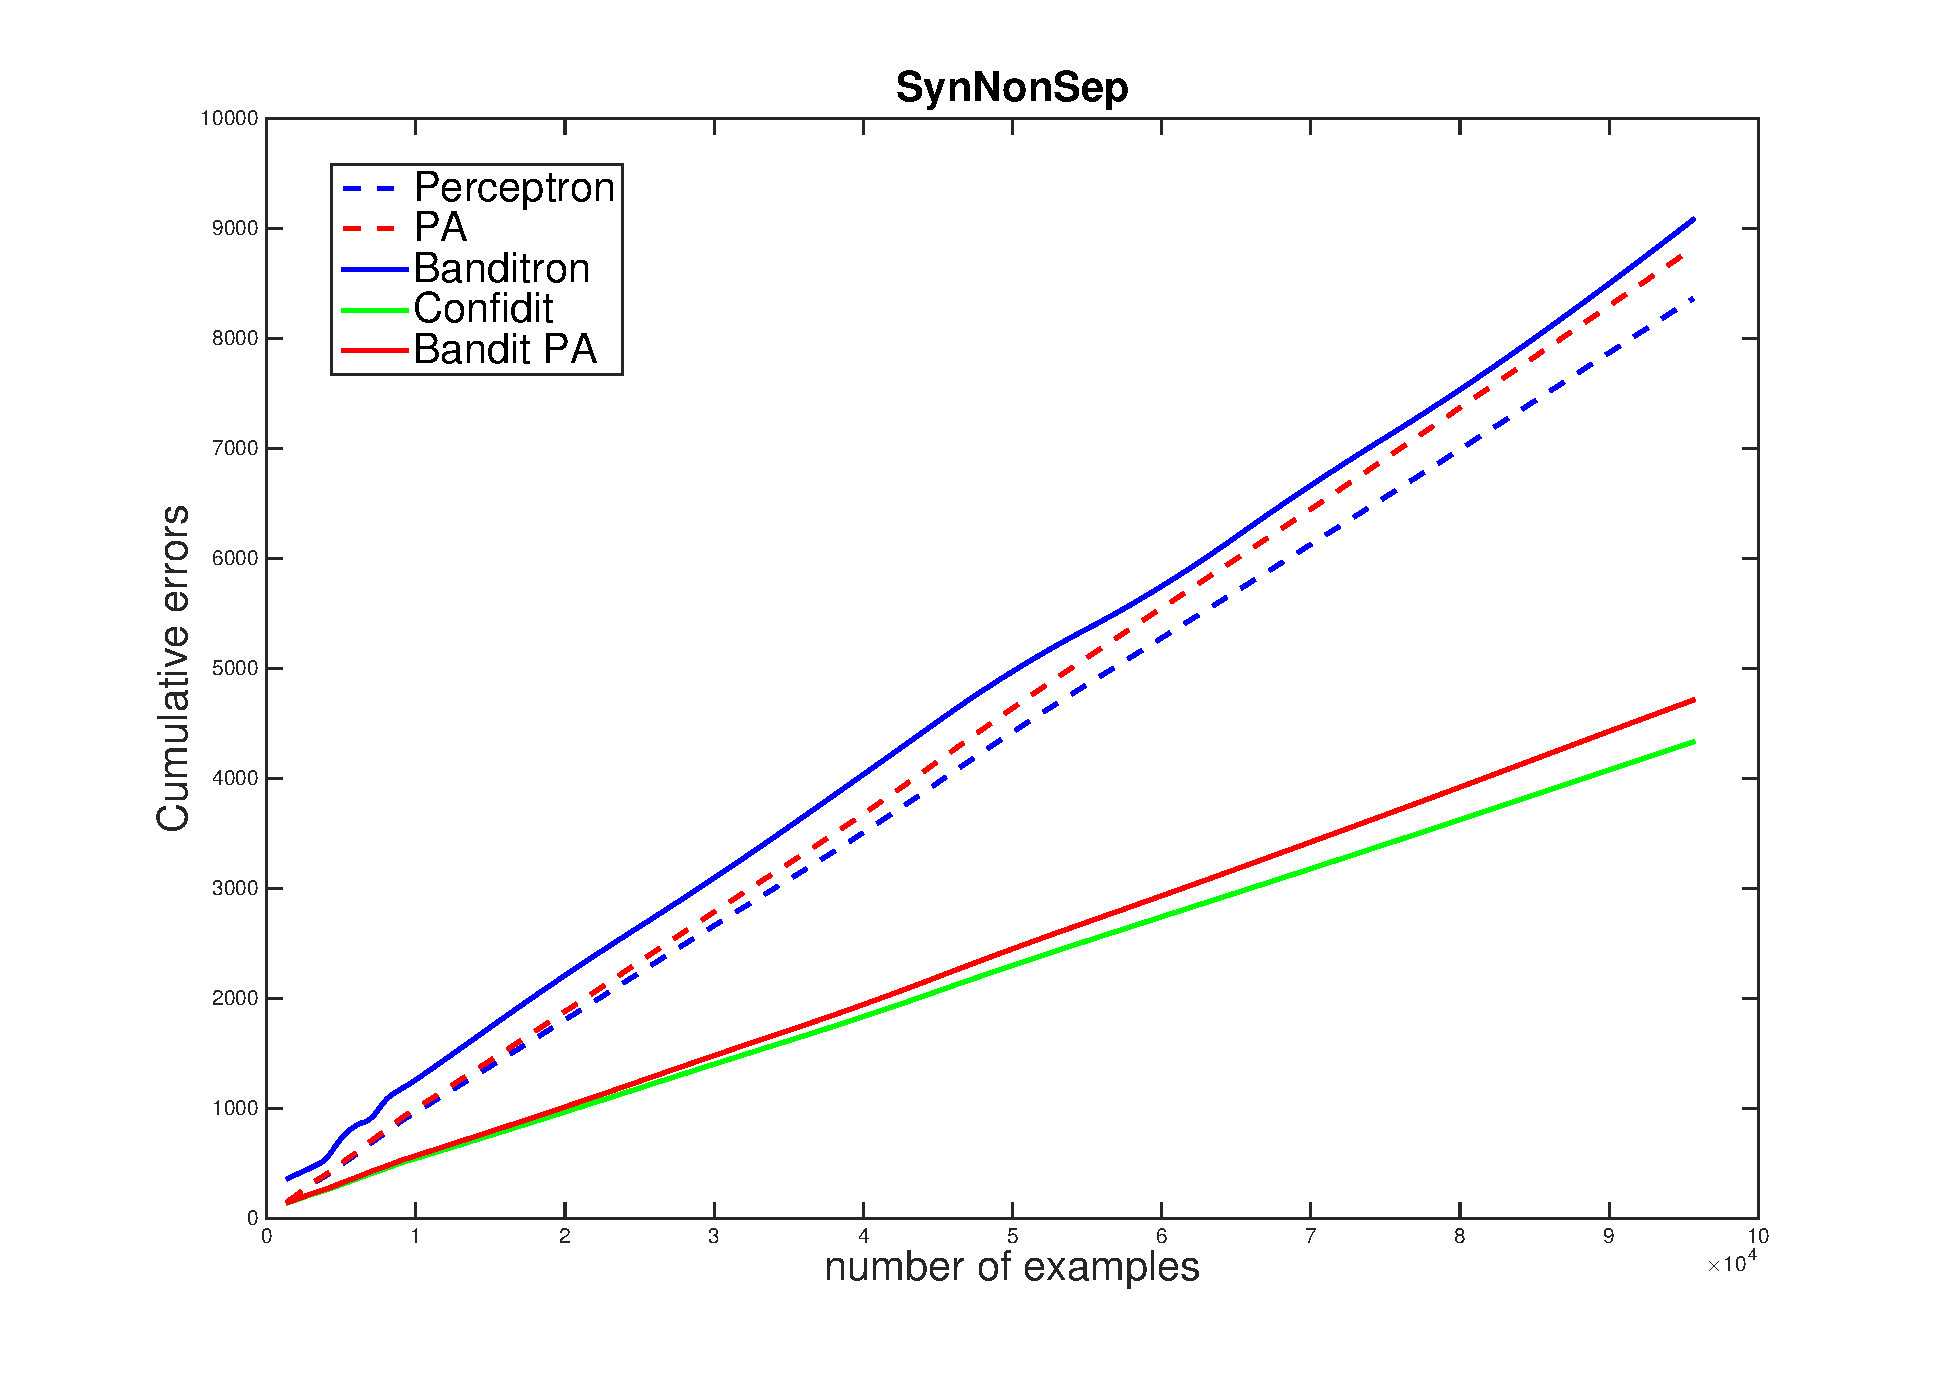
\includegraphics[scale = 0.4]{figs/SynNonSep.eps}
%	}
%	\caption{Cumulative Errors on the synthetic data set of SynNonSep.}
%	\label{pic:BPASNS}
%\end{figure}
%\begin{figure}[h!]
%	\centerline{
%		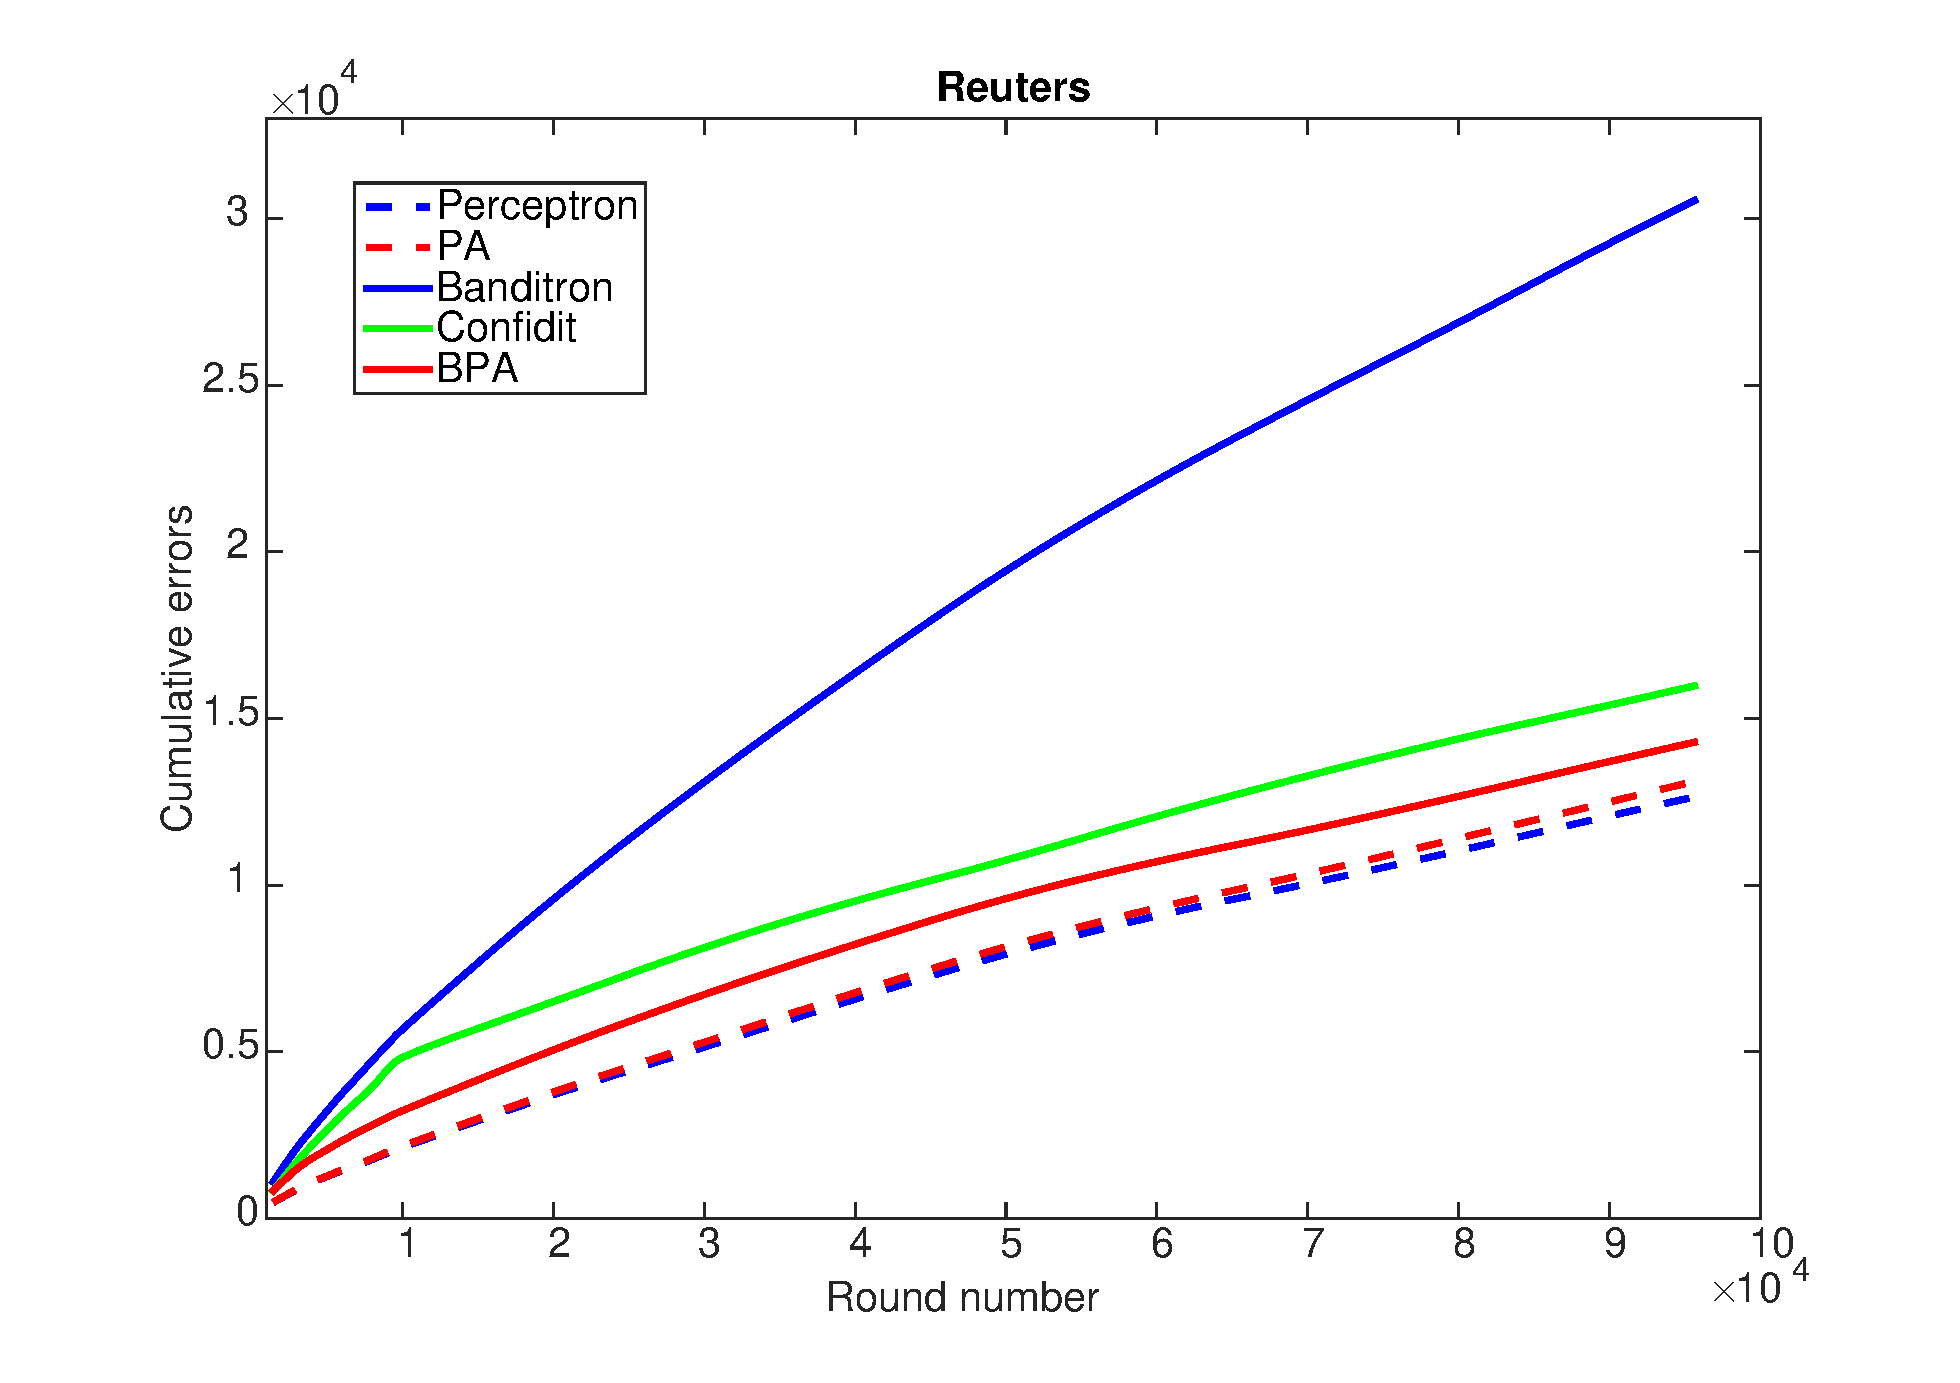
\includegraphics[scale = 0.4]{figs/RCV1_v2_53class.eps}}
%	\caption{Cumulative Errors  on the real data set of RCV1-v2 (53 classes).}
%	\label{pic:BPARCV}
%\end{figure}
%
%\begin{figure}[h!]
%	\centerline{
%		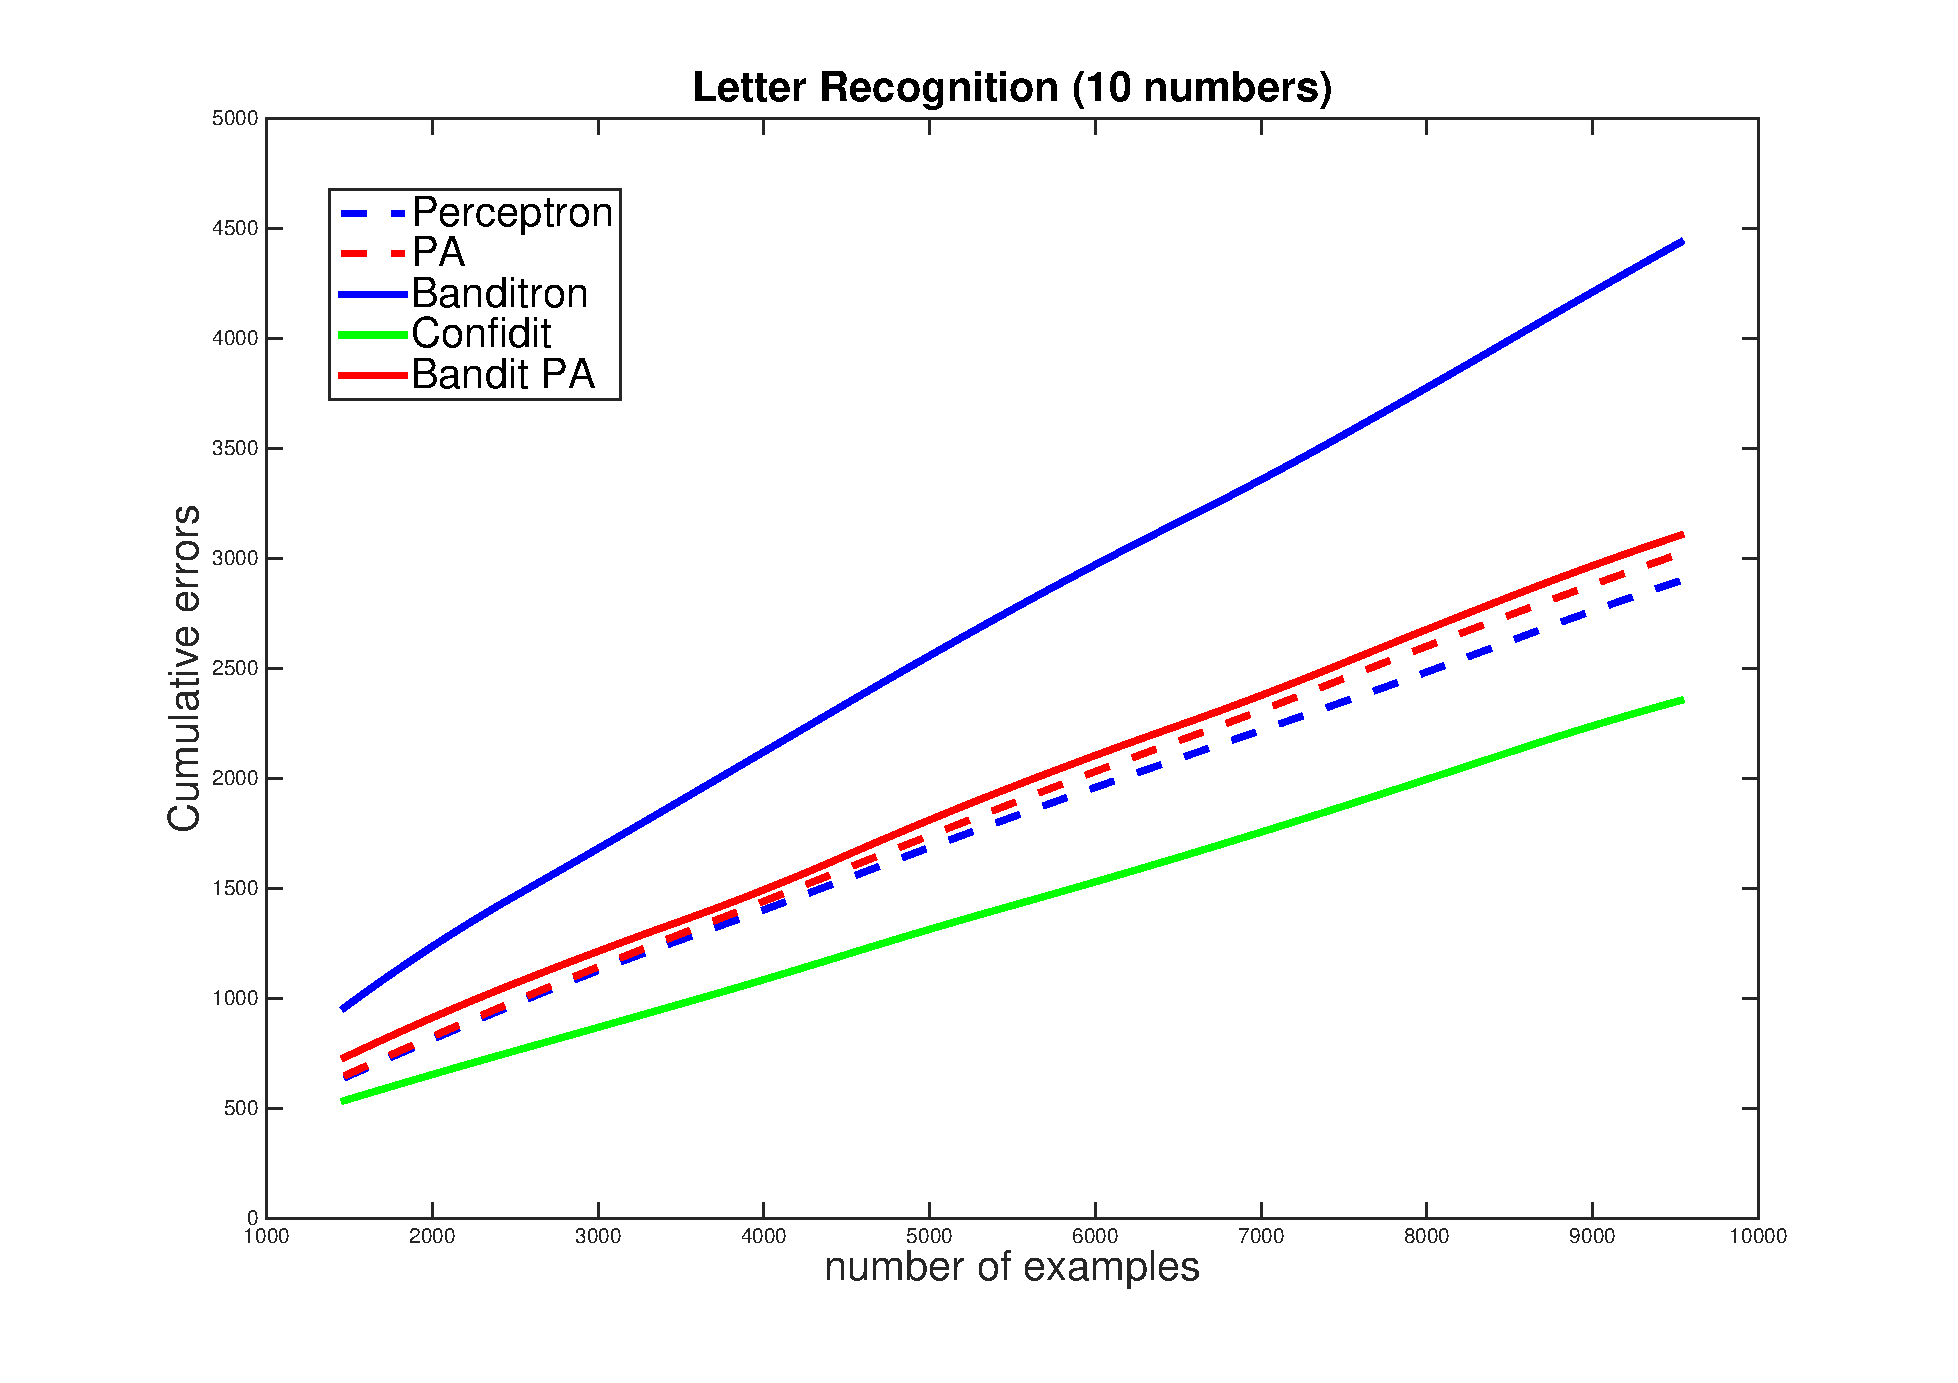
\includegraphics[scale = 0.4]{figs/10LR.eps}}
%	\caption{Cumulative Errors on the real data set of Letter Recognition (10 numbers).}
%	\label{pic:BPALR10}
%\end{figure}
%
%\begin{figure}[h!]
%	\centerline{
%		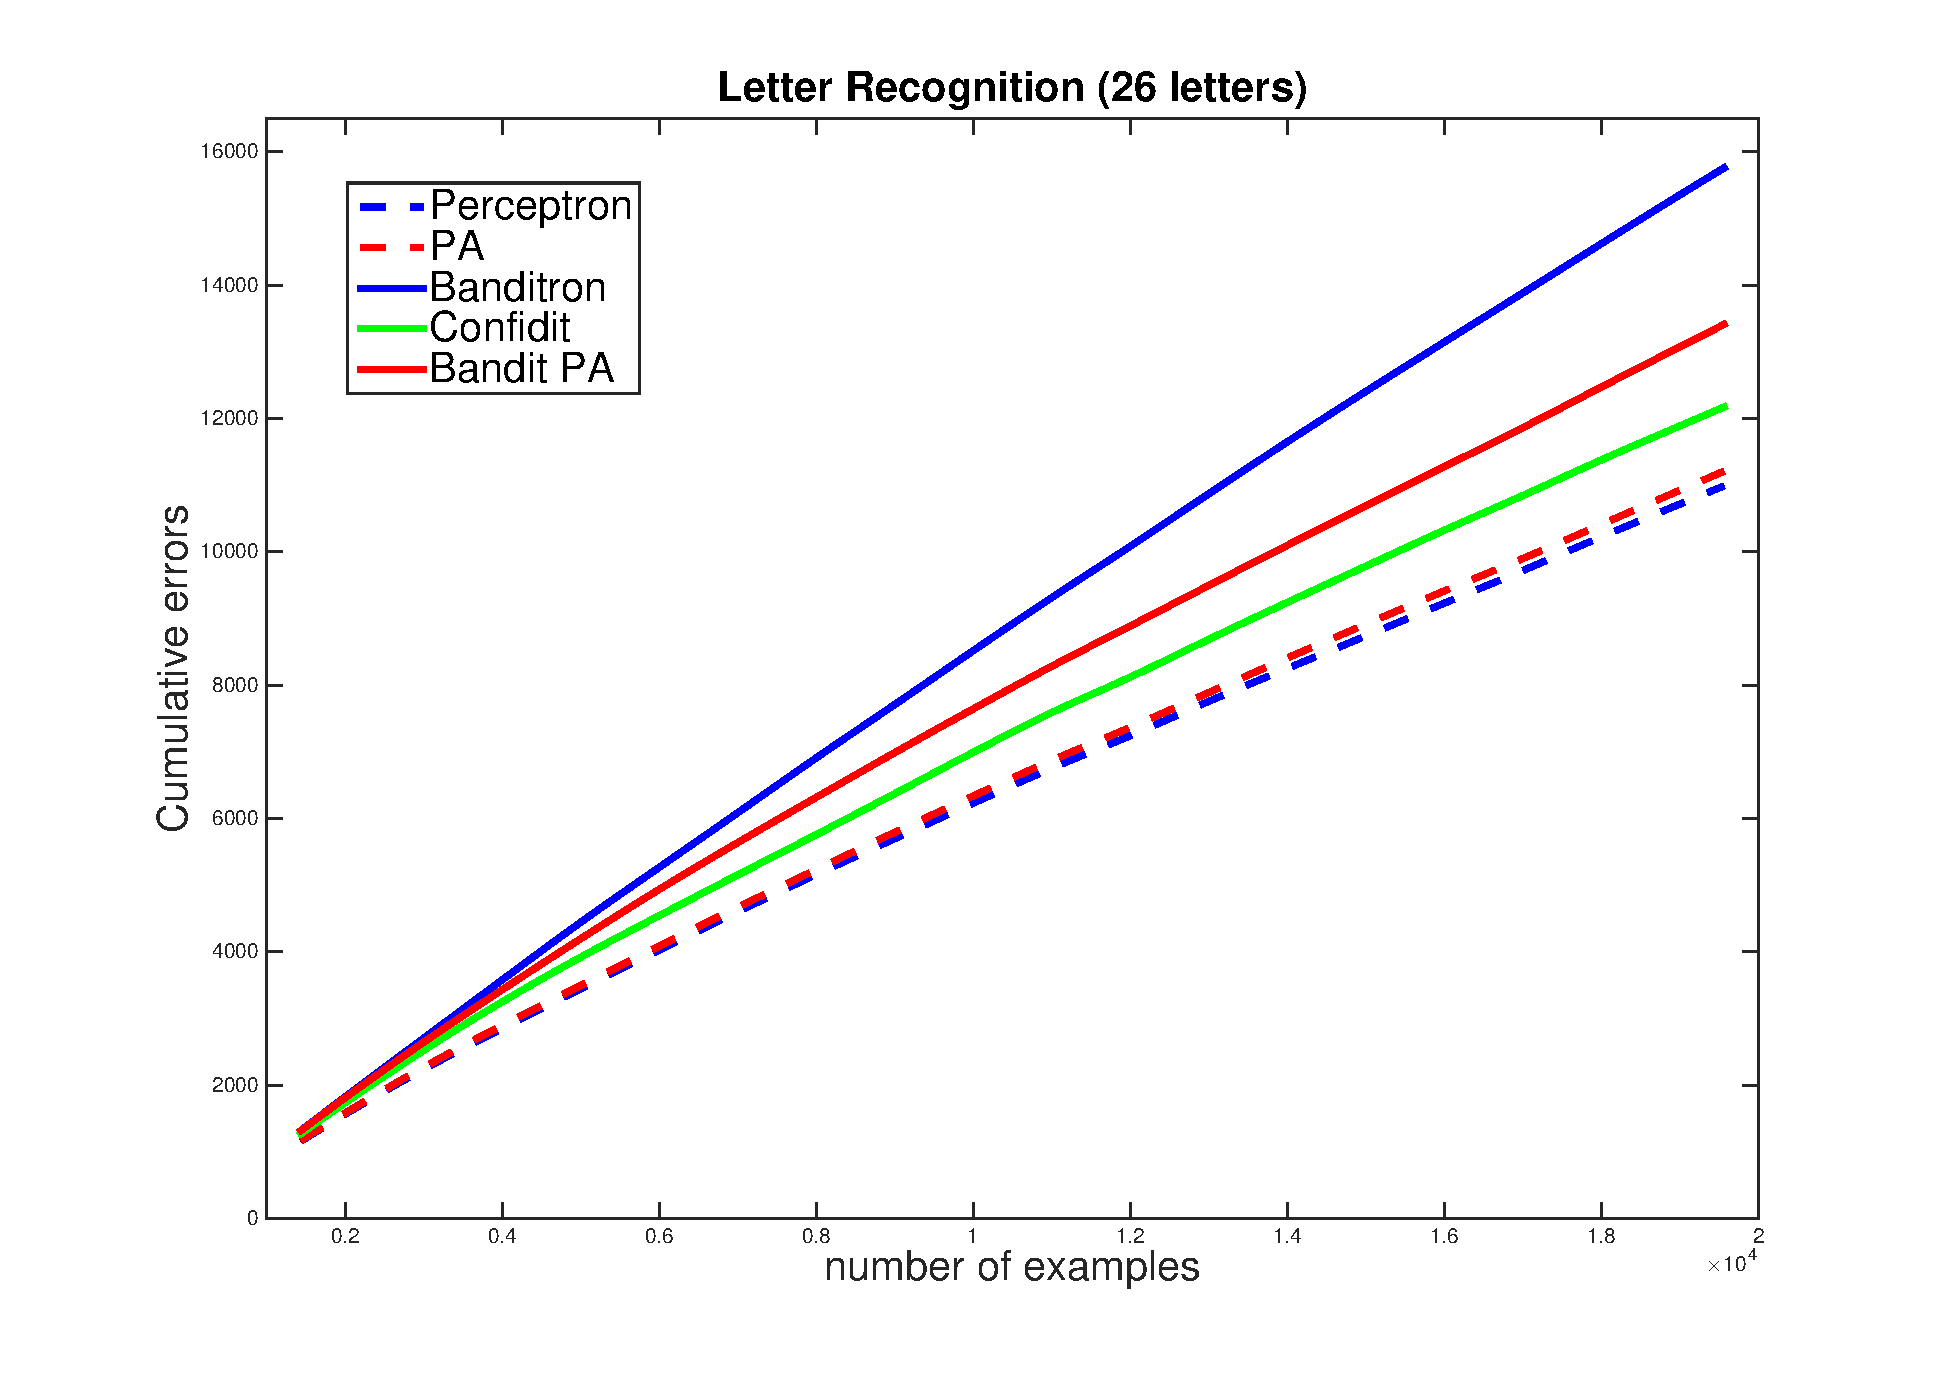
\includegraphics[scale = 0.4]{figs/26LR.eps}}
%	\caption{Cumulative Errors  on the real data set of Letter Recognition (26 Letters).}
%	\label{pic:BPALR26}
%\end{figure}
%
%\begin{figure}[h!]
%	\centerline{
%		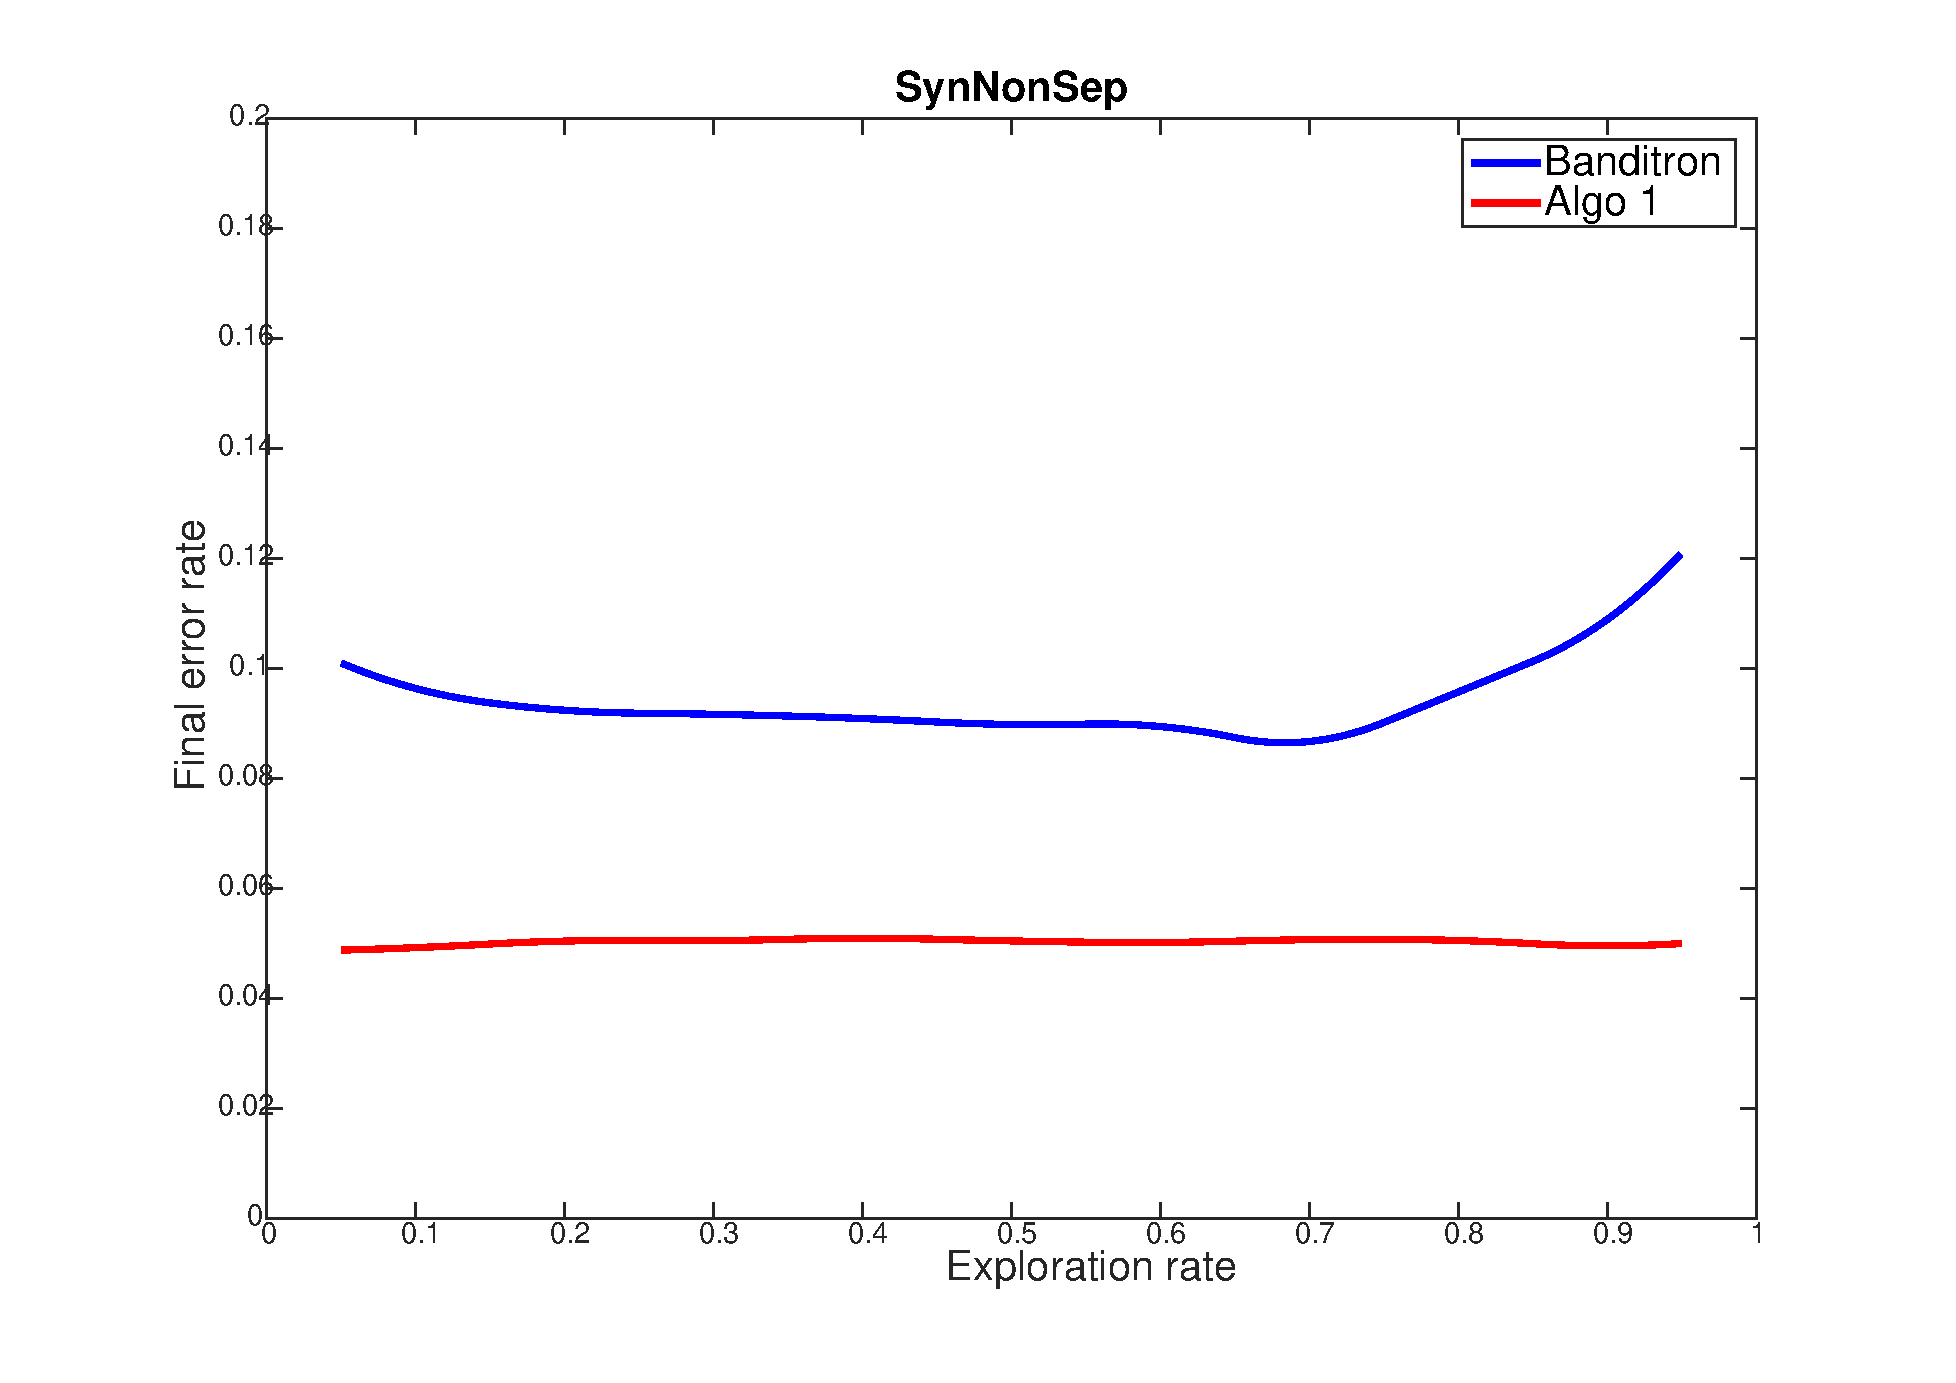
\includegraphics[scale = 0.4]{figs/SynNonSep_gamma.eps}}
%	\caption{Average error of Banditron and BPA for parameter's value $\epsilon$ on the data set of SynNonSep. }
%	\label{pic:BPASNSerr}
%\end{figure}
%
%\begin{figure}[h!]
%	\centerline{
%		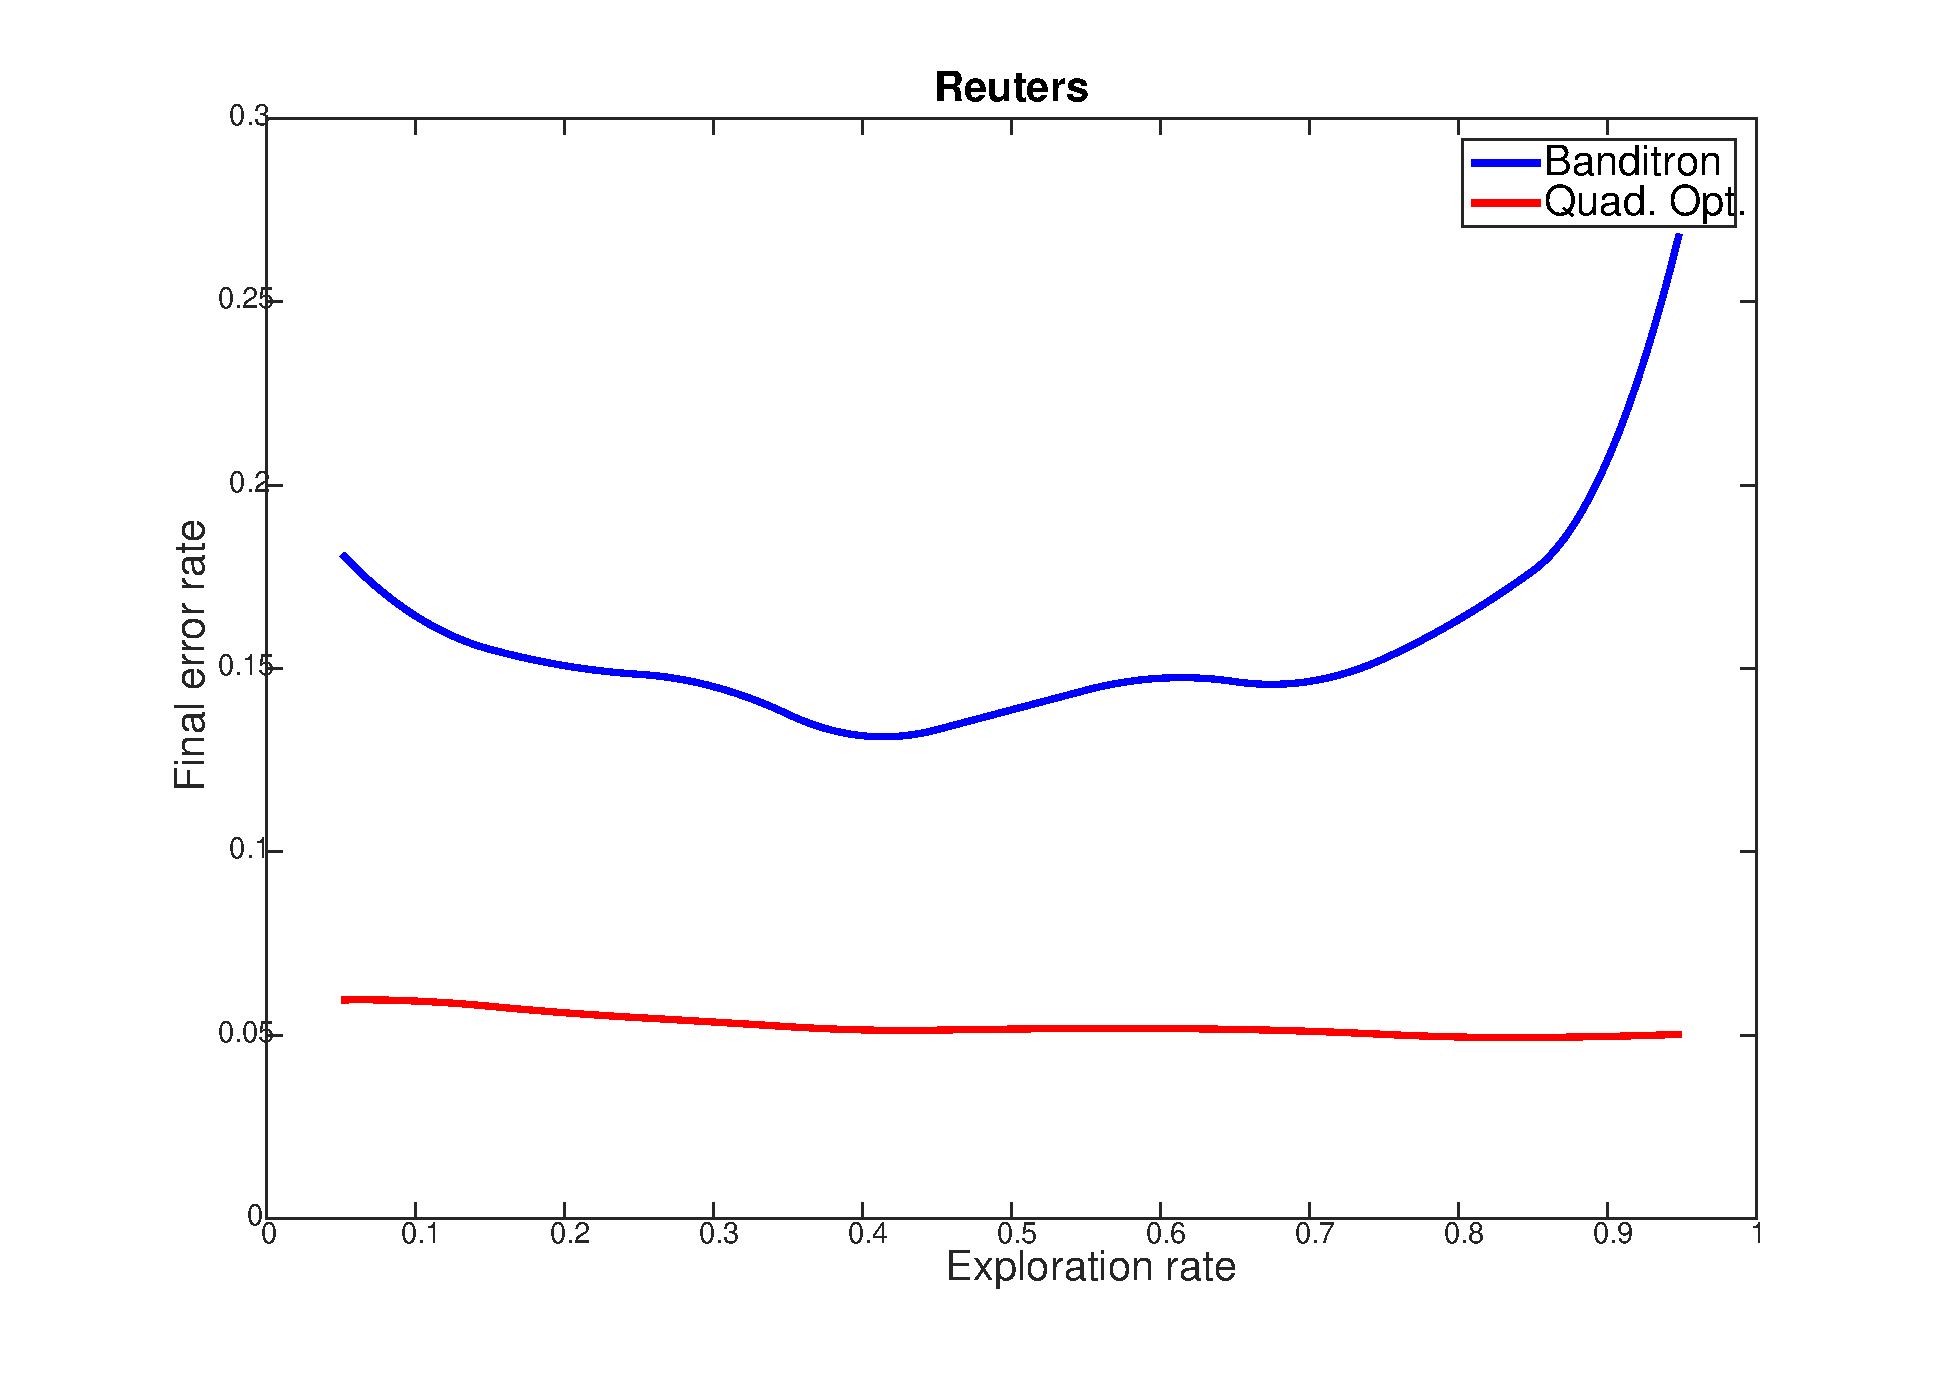
\includegraphics[scale = 0.4]{figs/Reuters_gamma.eps}}
%	\caption{Average error of Banditron and BPA for parameter's value $\epsilon$ on the data set of Reuters.}
%	\label{pic:BPARCVerr}
%\end{figure}
%
%\begin{figure}[h!]
%	\centerline{
%		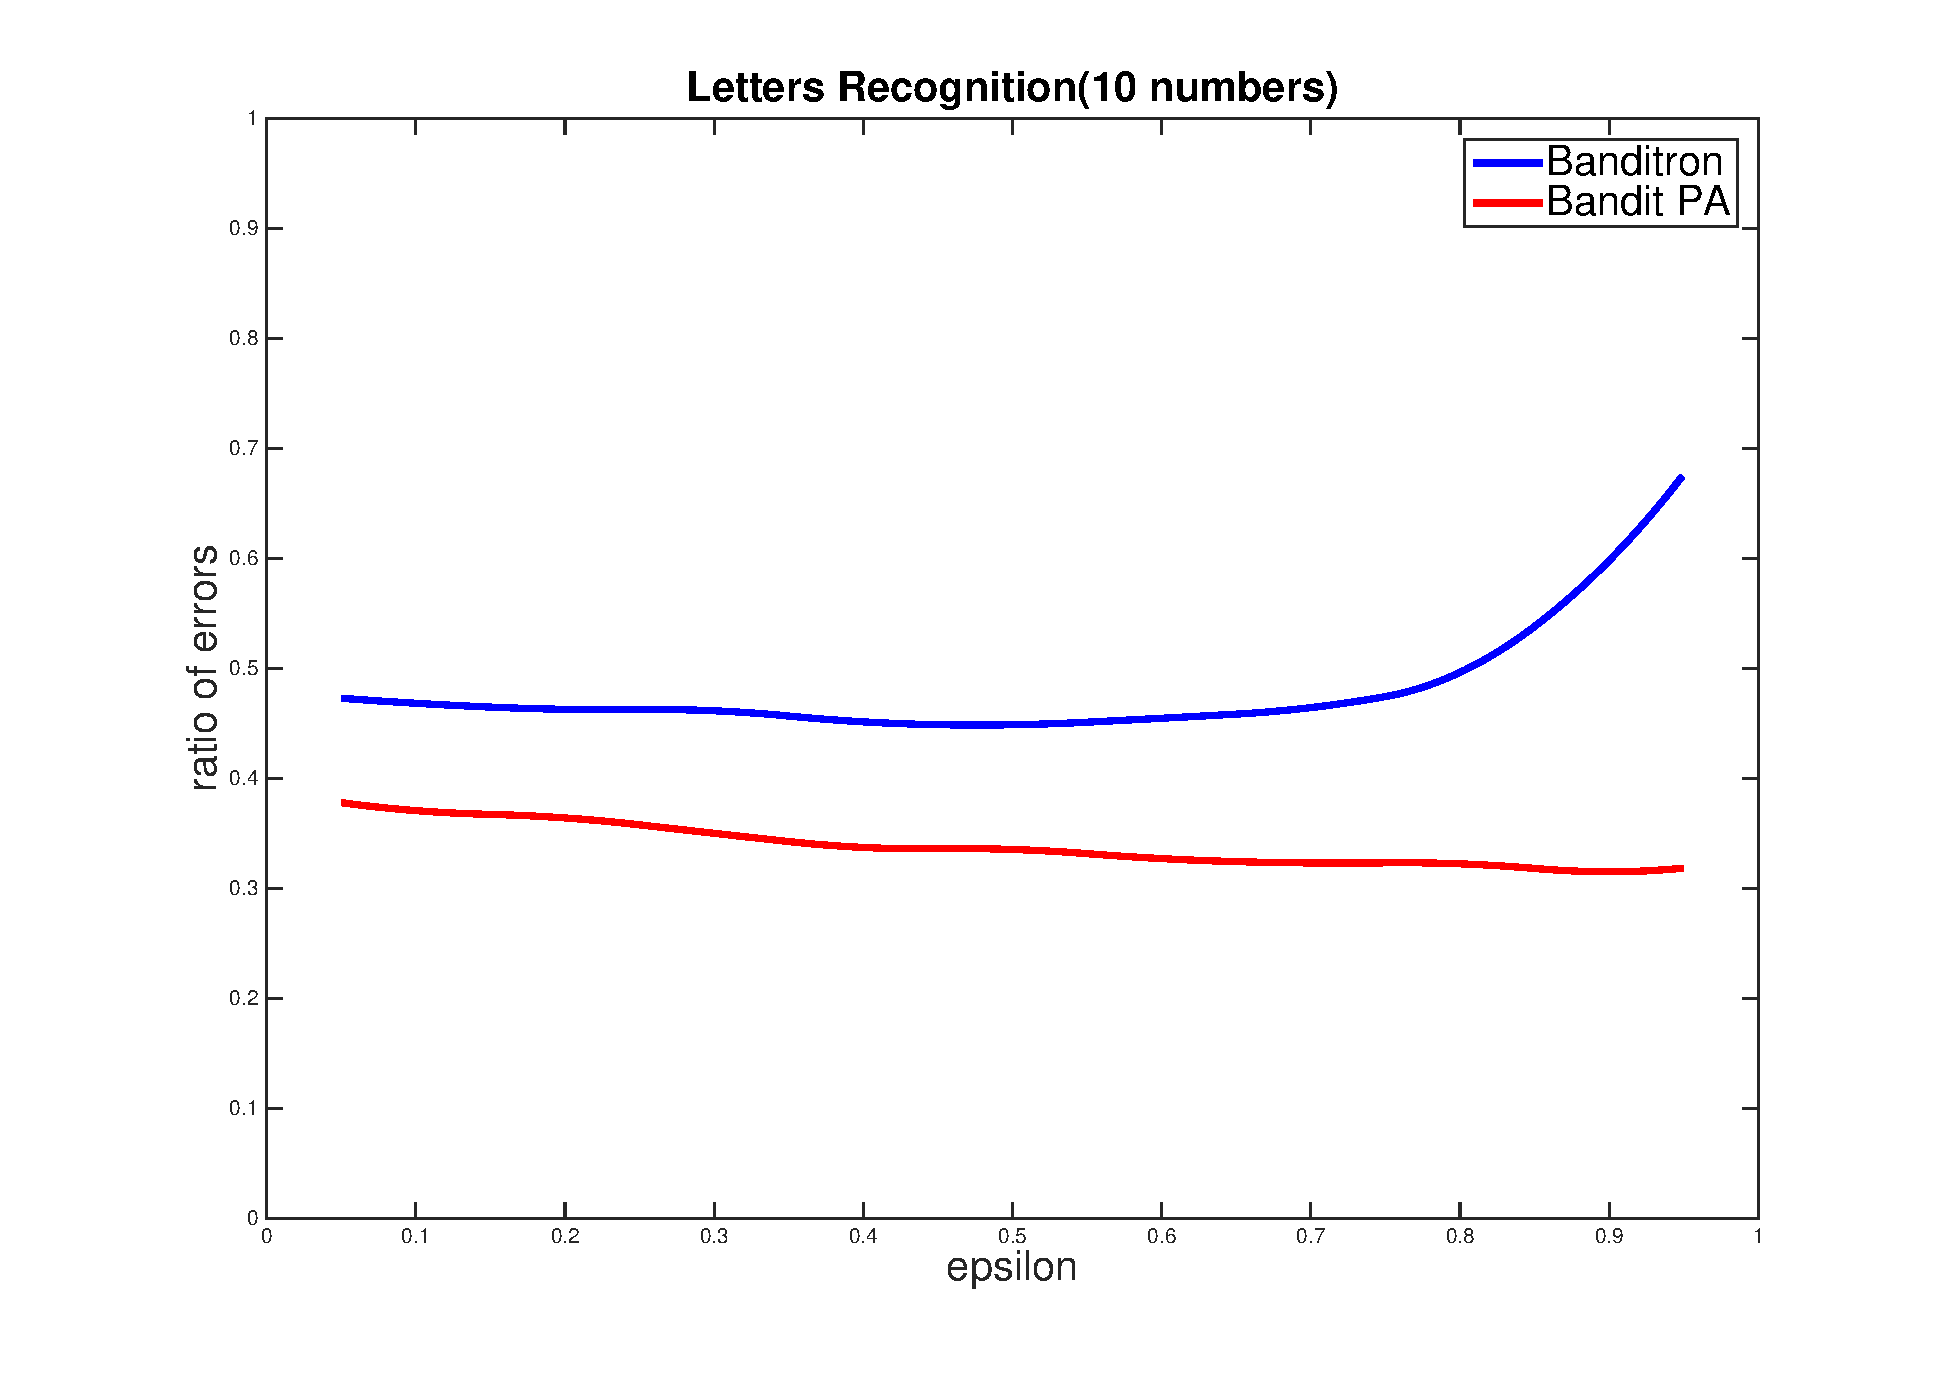
\includegraphics[scale = 0.4]{figs/10LR_gamma.eps}}
%	\caption{Average error of Banditron and BPA for parameter's value $\epsilon$ on the data set of Letter Recognition.}
%	\label{pic:BPALRerr}
%\end{figure}
%
%
%\subsection{Non-linearly separable datasets}
%
%In this section, we take two datasets to evaluate and analyze the effect of these algorithm in Reproducing Kernel Hilbert Space.
%
%\vspace{1.5ex}
%\textbf{Data description}
%The first dataset denoted by Pendigits, is a real data and created by E.Alpaydin and Fevzi.Alimoglu \cite{alimoglu1996combining,Alimoglu96methodsof}. 
%It  collected 250samples from 44 writers. All writers are asked to write 250 digits in random order inside boxes of 500 by 500 tablet pixel resolution. 
%Here, the dataset is part of original one. It contains 7494 instances, 16 features and 10 classes. 
%
%The second dataset denoted by `Segment'\cite{Lichman:2013}. This dataset contains 2310 instances, all of them were drawn randomly from a database of 7 outdoor images. The images were handsegmented to create a clasification for every pixel. Each instance is a $3\times 3$ region. It's a real dataset, with 19 features and 7 classes. More details could be referred to the data site ``UCI''.
%
%\vspace{1.5ex}
%%\textcolor{red}{OK-- Il faut donner la formule des noyaux lineaire et Laplace}
%\textbf{Algorithm}
%Here, we take algorithms Banditron (in RKHS), KBPA and KSGD to compare. In order to perform the effect of RKHS, we choose KBPA in linear model as the reference object and choose \textbf{Laplace} for the kernel function. Its form looks like the following formulate.
%\[K_{Laplace}(x,y) = \exp{\left(-\frac{\parallel{x-y}\parallel}{\sigma}\right)}\]
%So, all participant algorithms contains: KBanditron, KBPA (linear), KBPA (Laplace), and KSGD (Laplace). For each dataset, the parameter of kernel function is different. By cross-validation way, we choose $\eta = 1$ of model `Laplace' for dataset Pendigits and $\eta = 10$ for dataset `Segment'. For KSGD, the truncated number is 500 for dataset Pendigits, and 200 for Segment.
%
%\vspace{1.5ex}
%\textbf{Result}
%We mainly analyze these experiments from the following aspects. 
%
%Average training time for each instance:  we observe the training time of every instance $\{t_1,t_2,\dots,t_n\}$; then divide 100 ordering examples into one group $g_1 = \{t_1,\dots,t_{100}\}$,
%$\dots$, $g_i = \{t_{1+100*(i-1)},\dots, t_{100*i}\}$; finally, the average training time for instances of group $g_i$ can be calculated by $\overline{t_i} = \frac{1}{100}\sum_{s=1+100*(i-1)}^{100*i} t_s$. 
%
%Average error rate: $e_i = \sum_{s=1+100*(i-1)}^{100\times i}\mathbf{1}_{\hat{y}_t = y_t}/100$ this measure is calculated by the same way.
%
%Cumulative Errors: calculate the total number of past errors.
%
%In Figure~\ref{pic:PKT}, it gives the result of average training time on based dataset ``Pendigits''.  From this result, the training time of three kernel algorithms increases linearly along with the number of training instances. Only the linear model is stable. From the theoretical perspective, Banditron always adds a new example passively for its support vector. Algorithm KSGD only adds a new example for its support vector if its classifier makes a bad prediction, otherwise the number of support vector is limited by the truncated parameter. Algorithm KBPA adds a new example for its support vector if and only if its predicted loss not equals to zero. So its number of support vector will increase all the time until it can make good prediction with no loss.
%
%In Figure~\ref{pic:PKM} and Figure~\ref{pic:PKCM}, accumulative errors of algorithm KBPA firstly tend to a stable, others still increase linearly. That is because KBPA accumulates all good support vectors, KSGD only accumulates several recent support vectors and Kernel Banditron always accumulates new instance as negative support vector.
%
%In Figure~\ref{pic:SKT}, it is about the average training time on dataset ``Segment''.  The training time of Kernel Banditron still increases linearly, while the training time of KSGD and KBPA are as stable as linear model after a small period of increasing linearly. KSGD reaches the limited number of support vector, and KBPA quickly gets enough support vectors to make a good prediction. It could show that this dataset is separable. 
%
%In Figure~\ref{pic:SKM} and Figure~\ref{pic:SKCM}, we can observe that KBPA and KSGD performed obviously better than the other two.  Two kernel algorithms have ability to solve non-linear classification with Bandit Feedback. Considering the scale of classifier, we can use more efficient algorithm KBPA if dataset is separable, otherwise we use KSGD.
%
%\begin{figure}[h!]
%	\centerline{
%		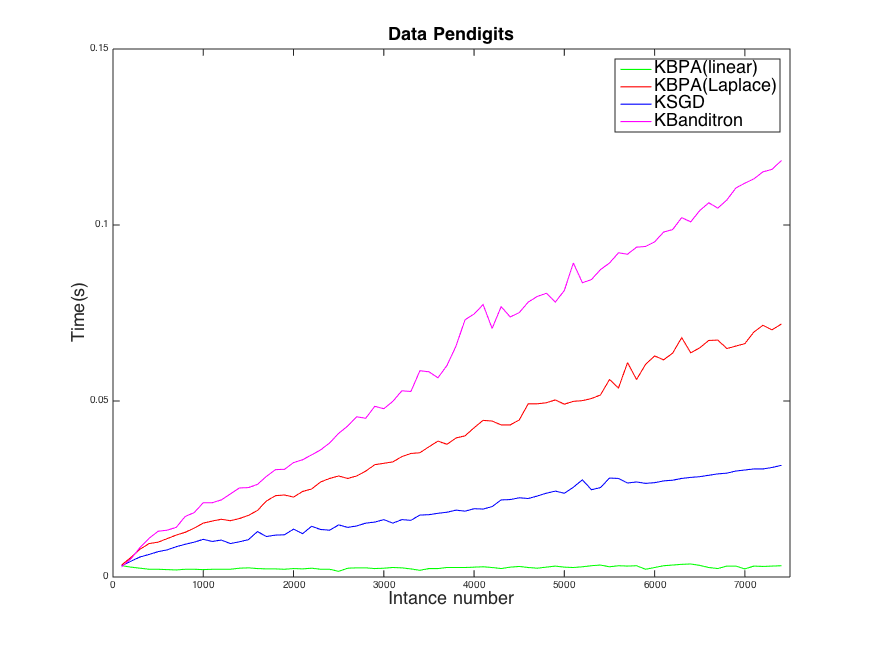
\includegraphics[scale = 0.4]{figs/Pendigits_kernel_T.png}
%	}
%	\caption{Average training time for each instance of Data Pendigits.}
%	\label{pic:PKT}
%\end{figure}
%
%\begin{figure}[h!]
%	\centerline{
%		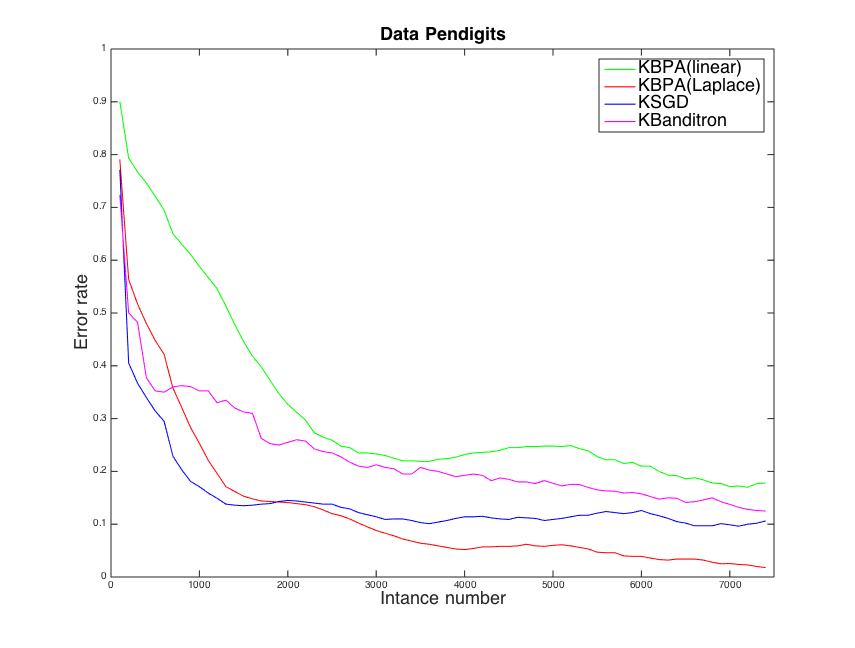
\includegraphics[scale = 0.4]{figs/Pendigits_kernel_M.png}}
%	\caption{Average error rate for each instance of Data Pendigits}
%	\label{pic:PKM}
%\end{figure}
%
%\begin{figure}[h!]
%	\centerline{
%		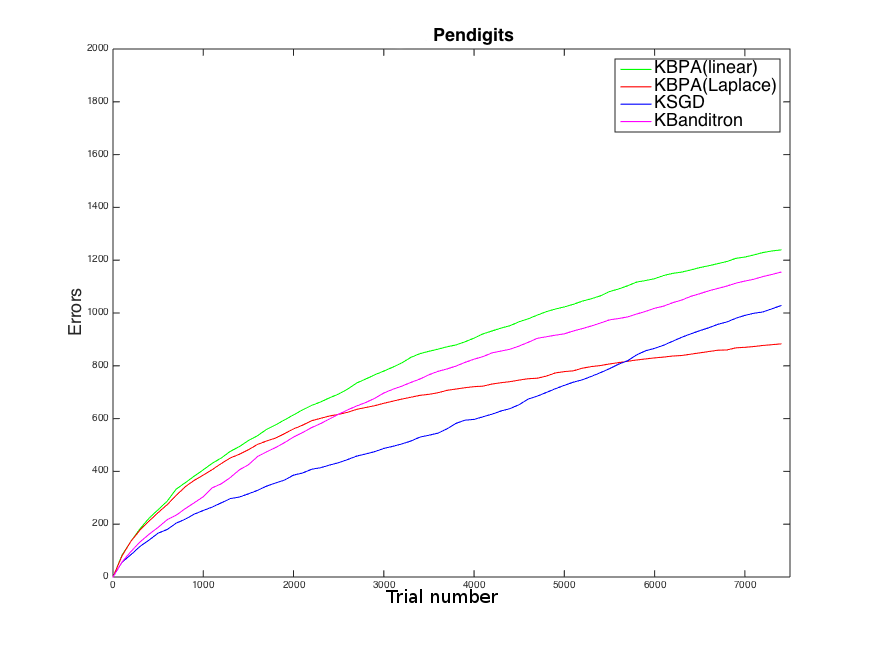
\includegraphics[scale = 0.4]{figs/Pendigits_kernel_CM.png}}
%	\caption{Cumulative Errors of Data Pendigits}
%	\label{pic:PKCM}
%\end{figure}
%
%%\begin{figure}[h!]
%%\label{pic:PKR}
%%\centerline{
%%\includegraphics[scale = 0.4]{fig05/mc/Pendigits_kernel_R.png}}
%%\caption{Cumulative loss of Data Pendigits}
%%\end{figure}
%
%\begin{figure}[h!]
%	\centerline{
%		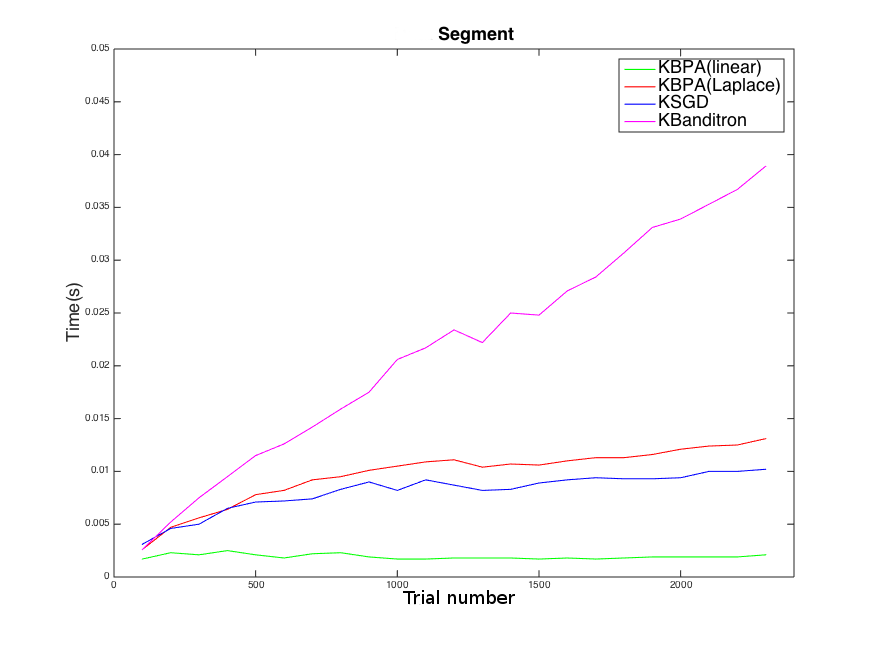
\includegraphics[scale = 0.4]{figs/Segment_kernel_T.png}}
%	\caption{Average training time for each instance of Data Segment.}
%	\label{pic:SKT}
%\end{figure}
%
%\begin{figure}[h!]
%	\centerline{
%		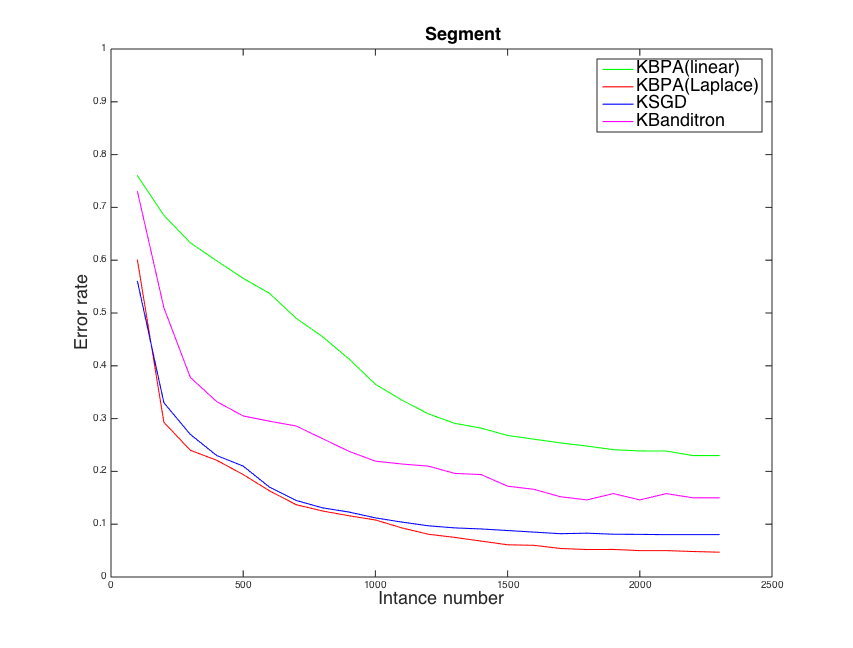
\includegraphics[scale = 0.4]{figs/Segment_kernel_M.png}}
%	\caption{Average error rate for each instance of Data Segment}
%	\label{pic:SKM}
%\end{figure}
%
%\begin{figure}[h!]
%	\centerline{
%		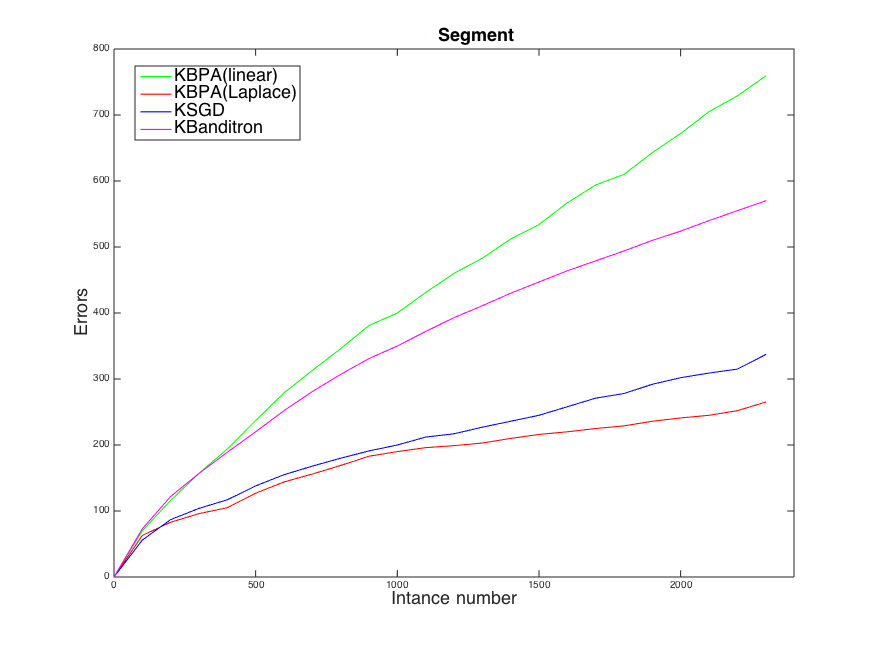
\includegraphics[scale = 0.4]{figs/Segment_kernel_CM.png}}
%	\caption{Cumulative Errors of Data Segment}
%	\label{pic:SKCM}
%\end{figure}
%
%%\begin{figure}[h!]
%%\label{pic:SKR}
%%\centerline{
%%\includegraphics[scale = 0.4]{fig05/mc/Segment_kernel_R.png}}
%%\caption{Cumulative loss of Data Segment}
%%\end{figure}
%%\subsection{Conclusion}
\section{Conclusion}
\label{sec:conclusion}

We have shown that a conservative reduction of the OVA hinge-loss  provides effective and lightweight solutions to the online bandit classification problem (defined by \cite{kakade2008efficient}). 
For instance, when adapting the passive aggressive setup as proposed in the supervised case by \cite{crammer2006online}, 
%i.e. sequentially solving local quadratic optimization problems,
we prove  similar bounds on the observed cumulative squared loss. 
Here, however, the bound is not an upper bound of the classification error. Additional regularity assumptions, such as observation sets convexity, or a partly uniform sampling of the realization space, need to be considered to provide comparable error upper bounds. In addition, as in \cite{crammer2006online}, a misclassification stiffness parameter $C$ need to be set to reach $O(\sqrt{T})$ regret in the stationary case.  

The numerical simulations provide favorable results on both large scale text mining  datasets and on more classical non-linearly separable machine learning datasets. 
When comparing our approach with the Banditron, a first result is the exploration parameter $\varepsilon$ insensitivity, allowing to consider $\varepsilon$ decrease  over time in practical implementations. 


A comparison with the contextual bandit approach, using second order statistics and confidence interval estimates (see \cite{crammer2013multiclass}), is also shown favorable to our approach on a scale-realistic dataset, while owning a much lesser complexity. More surprisingly, a good resilience to label noise is also shown on a synthetic dataset, for the method was not specifically designed to address this aspect. 

While most contextual bandit setups concentrate to large-scale text-mining and recommendation datasets, we actually implemented a kernel approach on more traditional non-linearly separable datasets, and show it effective when both considering sparsity (such as addressed by \cite{kivinen2004online}), and final classification accuracy, with, for instance, a close to state-of-the-art 98\% final accuracy observed after one pass on the Pendigits 10-class problem.


From a more general standpoint, the bandit classification problem implements a form of active learning in scarcely labeled environments, with a limited (1 bit) information budget at each round. This budget is here used in the form of a single margin constraint under the OVA setup. Solving sequentially the observed margin constraints is then expected to solve in approximation the total (unobserved) set of margin constraints, provided enough redundancy is present in the data. This approach is exactly fitted to the specific stationary classification tasks considered here, and for that reason is shown to powerfully compete with the more demanding confidence-based second-order bandits setups. On one side, the OVA reduction may even generalize to slightly more demanding tasks, like the multi-label setup generally considered in recommender systems. On the other side, it should be overcome as soon as non-stationary and adversarial settings are considered.
The H-horizon window-based approach, as proposed by \cite{kivinen2004online}, may in some cases be substituted, for it  shows both effectiveness, sparsity and adaptivity in our simulations.  
    


%{\color{green}
%
%
%1. les bornes obtenues
%
%2. approx memes perf que confidit (ou ordre 2) avec en plus : (1) une moindre complexité et (2) la parcimonie des mises à jour. 
%
%Generalités : le 1-bit feedback est specifique --> simplifie les preuves (preuves directement transposables)
%
%overconstrained/subsampling problem
%
%no optimal set point for epsilon (free choice)
%
%policy independent}
%
%We compare in this paper several online learning setups that apply to the case  when the expected label is not fully disclosed, but instead a single bit, telling whether the current output is correct or incorrect, is provided. The  absence of explicit label information XXX to randomly sample the label space, in the manner of contextual bandits, and consider the exploration exploitation trade-off in the decision process. 
%
%%Nous avons proposé dans cet article un nouvel algorithme d'apprentissage en ligne de classifieurs multiclasses dans le cas où l'information de classification est binaire (réponse correcte ou incorrecte). L'absence d'information de label explicite conduit à échantillonner de manière aléatoire l'espace des labels, sur le modèle des bandits contextuels. L'approche utilisée ici pour l'exploration est $\varepsilon$-glouton, soit une alternance entre échantillonnage uniforme et exploitation. 
%
%L'algorithme développé repose  sur l'optimisation à chaque essai d'une fonction de coût spécifique, sur le modèle de l'approche ``Passive Agressive'' proposée par \cite{crammer2006online}. 
%L'analyse mathématique permet de mettre en évidence des bornes sur la somme des coûts cumulés, à la fois dans le cas séparable et dans le cas non séparable, comparables aux bornes obtenues dans le cas supervisé.
%
%Les expériences numériques confirment le bon comportement de l'algorithme d'apprentissage, à la fois sur des données de grande dimension et sur des jeux de données non-linéairement séparables. Tout en présentant une complexité algorithmique similaire, notre approche dépasse systématiquement les performances de l'algorithme du Banditron \cite{kakade2008efficient}. En particulier, nous observons une faible sensibilité au taux d'exploration $\varepsilon$, soit une conservations des performances depuis l'échantillonnage pur jusqu'à l'exploitation ``gloutonne'' de la réponse du classifieur. Cette propriété permet en conditions réelles d'envisager une implémentation de l'algorithme avec un $\varepsilon$ décroissant au cours de l'apprentissage.    
%
%Les courbes d'apprentissage montrent des performances similaires aux méthodes d'ordre 2, tout en présentant une complexité linéaire en espace. 
%Cette complexité faible permet en particulier d'appliquer aisément cette approche aux données de grande dimension. Les expériences montrent également un bon comportement dans le cas où le nombre de classes est assez élevé (ici 53 classes dans le cas de la base Reuters).  
%Dans le cas où les données ne sont pas linéairement séparables, l'algorithme présente une bonne parcimonie, permettant d'éviter une croissance trop importante du nombre de vecteurs supports au cours de l'apprentissage.
%
%Plus généralement, ces résultats illustrent le fait qu'une information de classification minimale (ici binaire) se révèle suffisante pour un apprentissage multi-classes performant, offrant en particulier des bornes de convergence comparable en ordre de grandeur à celles reposant sur une information de classification complète.
%
%
%
%%In the next section, we will take BPA to deal with non-linear data sets  by combining the Kernel method. 
%
%
%
%%Reading :
%%Fundamental Limits of Online and Distributed Algorithms for Statistical Learning and Estimation Ohad Shamir (NIPS’14)
%%Many machine learning approaches are characterized by information constraints on how they interact with the training data. These include 
%%memory and sequential access constraints (e.g. fast first-order methods to solve stochastic optimization problems); 
%%communication constraints (e.g. distributed learning); 
%%partial access to the underlying data (e.g. missing features and multi-armed bandits) 
%%algorithm with small memory footprint
%%The standard implementation of many common learning tasks requires memory which is super-linear in the data dimension
%%The need for fast and scalable learning algorithms has popularised the use of online algorithms, which work by sequentially going over the training data, and incrementally updating a (usually small) state vector
%%There has also been considerable interest in online learning with partial information, where the learner only gets partial feedback on his performance. This has been used to model various problems in web advertising, routing and multiclass learning. Perhaps the most well-known case is the multi-armed bandits problem with many other variants being developed, such as contextual bandits, combinatorial bandits, and more general models such as partial monitoring [Bubeck, Cesa-Bianchi]
%%sequential decisions
%
%
%%% The Appendices part is started with the command \appendix;
%%% appendix sections are then done as normal sections
%%% \appendix
%
%%% \section{}
%%% \label{}
%
%%% If you have bibdatabase file and want bibtex to generate the
%%% bibitems, please use
%%%
%
%%% else use the following coding to input the bibitems directly in the
%%% TeX file.
%
%% %\begin{thebibliography}{00}
%
%%% \bibitem[Author(year)]{label}
%%% Text of bibliographic item
%
%%% \bibitem[ ()]{}
%
%% %\end{thebibliography}
\section*{Acknowledgements}

This work was supported by the China Studentship Council (CSC). Thanks to Liva Ralaivola (LIF, Marseille, France) for fruitful discussions.

\appendix
\section{Proof of Theorem \ref{theo:BPAT1}}\label{app:thm1}

\begin{proof}
	Define $\Delta_t$ to be:
	\[\Delta_t = \parallel{W_{t-1}-U}\parallel^2-\parallel{W_t-U}\parallel^2\]
	Summing $\Delta_t$ over all $t$ from 1 to $T$ collapses to:
	\begin{align}
	\sum_{t=1}^{T}\Delta_t &= \sum_{t=1}^{T} \left( \parallel{W_{t-1} - U}\parallel^2-\parallel{W_t - U}\parallel^2 \right)\nonumber\\ 
	&= \parallel{W_0 - U}\parallel^2-\parallel{W_T-U}\parallel^2\nonumber
	\end{align}	
	Given that $W_0 = \vec{0}$, 
	\begin{equation}
	\label{equa:delta}
	\sum_{t=1}^{T}\Delta_t = \parallel{U}\parallel^2 - \parallel{W_T-U}\parallel^2 \leqslant \parallel{U}\parallel^2 
	\end{equation}
	
	Using the definition of update : %in Eq.\ref{eq:,
	\begin{align}
	\Delta_t = -2\left\langle W_{t-1} - U, (2f_t-1)\frac{l_t}{\parallel{x_t}\parallel^2}X_t^{\tilde{y}_t}\right\rangle 
	- \left\| \frac{l_t}{\parallel{x_t}\parallel^2}X_t^{\tilde{y}_t}\right\|^2
	\nonumber
	\end{align}
	%With    and   ,
	So, taking $\parallel{X_t^{\tilde{y}_t}}\parallel = \parallel x_t\parallel$, it comes:

	\begin{align}
	\Delta_t =& 2l_t\frac{(1-2f_t)\langle W_{t-1}, X_t^{\tilde{y}_t}\rangle - (1-2f_t)\langle U, X_t^{\tilde{y}_t}\rangle}{\|x_t\|^2}
	-\frac{l_t^2}{\parallel{x_t}\parallel^2}\nonumber
	\end{align}
	Then, noting that:
		\begin{itemize}
			\item[] $l_t = [1+(1-2f_t)\cdot\langle W_{t-1},X_t^{\tilde{y}_t}\rangle]_+$
			\item[] $l_t^{\ast} = [1+(1-2f_t)\cdot\langle U,X_t^{\tilde{y}_t}\rangle]_+$
		\end{itemize}
		that $\Delta_t = 0$ when $l_t = 0$, and that $l^*_t \geq  1+(1-2f_t)\cdot\langle U,X_t^{\tilde{y}_t}\rangle$, it comes : 
	\begin{align}
	\Delta_t\geqslant& 2l_t\frac{l_t - l_t^{\ast}}{\parallel{x_t}\parallel^2}-\frac{l_t^2}{\parallel{x_t}\parallel^2}\nonumber\\
	=& \frac{l_t^2-2l_t l_t^{\ast}}{\parallel x_t\parallel^2}\nonumber
	\end{align}
	Given that $U$ is such that $\forall t \in [1,...,T]$ , $l_t^{\ast} = 0$,
	%, following the Eq.~\ref{sumDelta},
	
	\[\Rightarrow \parallel{U}\parallel^2 \geqslant \sum_{t=1}^{T}\Delta_t \geqslant \sum_{t=1}^{T}  \frac{l_t^2}{\parallel{x_t}\parallel^2}
	\geqslant 
	\sum_{t=1}^{T}  \frac{l_t^2}{R^2}
	\]
	\[\Rightarrow\sum_{t=1}^{T} l_t^2 \leqslant R^2 \cdot \parallel{U}\parallel^2\]
\end{proof}

\section{Proof of Theorem \ref{theo:BPAT2}}\label{app:thm2}
\begin{proof}
	From the proof of Theorem \ref{theo:BPAT1}, 
	\[\sum_{t=1}^{T}l_t^2 \leqslant R^2\cdot \parallel{U}\parallel^2 + 2\sum_{t=1}^{T}l_t l_t^{\ast}\]
	To upper bound the right side of the above inequality, we denote $a_t = \sqrt{\sum_{t=1}^{T}l_t^2}$ and $b_t = \sqrt{\sum_{t=1}^{T}(l_t^{\ast})^2}$, 
	\begin{align}
	2(a_tb_t)^2-2(\sum_{t=1}^{T}l_tl_t^{\ast})^2 =& \sum_{i=1}^{T}\sum_{j=1}^{T}l_i^2(l_j^{\ast})^2+\sum_{i=1}^{T}\sum_{j=1}^{T}l_j^2(l_i^{\ast})^2 \nonumber\\
	&- 2\sum_{i=1}^{T}\sum_{j=1}^{T}l_il_jl_i^{\ast}l_j^{\ast}\nonumber\\
	=& \sum_{i=1}^{T}\sum_{j=1}^{T}(l_il_j^{\ast}-l_jl_i^{\ast})^2 \geqslant 0 \nonumber
	\end{align}
	
	\begin{align}
	\sum_{t=1}^{T}l_t^2 \leqslant R^2 \cdot \parallel{U}\parallel^2+2\sum_{t=1}^{T}l_tl_t^{\ast}\leqslant R^2 \cdot \parallel{U}\parallel^2+2a_tb_t\nonumber
	\end{align}
	then considering:
	\[a_t^2 -2 a_tb_t+b_t^2\leqslant R^2\parallel{U}\parallel^2+b_t^2\]
	%the largest possible $a_t$ respecting the inequality is $b_t+\sqrt{R^2\parallel{U}\parallel^2+b_t^2}$
	we obtain :
	\[a_t \leqslant b_t+\sqrt{R^2\parallel{U}\parallel^2+b_t^2}\]
	and using the fact that $\sqrt{a+b}\leqslant \sqrt{a}+\sqrt{b}$,
	\[a_t \leqslant R\parallel{U}\parallel+2 b_t\]
	so that :
	\[\sum_{t=1}^{T}l_t^2 \leqslant \left(R\parallel{U}\parallel+2 \sqrt{\sum_{t=1}^{T}(l_t^{\ast})^2}\right)^2 \]
\end{proof}
\section*{References}
\bibliographystyle{elsarticle-harv} 
\bibliography{main}


\end{document}

\endinput
%%
%% End of file `elsarticle-template-harv.tex'.
